\chapter{Vektoren}
\section{Definition}
\begin{mydef}Ein Vektor ist eine Äquivalenzklasse aller gleich langen und gleichgerichteten Pfeilen. Jeder Pfeil aus dieser Menge ist ein Repräsentant des Vektors.\end{mydef}
\section{Darstellung von Vektoren im $\mathbb{R}^2$}
Einen Repräsentanten $a$ eines Vektors stellen wir typischer mit einem Pfeil dar: $\vec{a}$. Dieser setzt sich aus einer x- und y-Koordinate zusammen. z.B:
\begin{equation*}
\vec{a} = \begin{pmatrix}x\\y \end{pmatrix} \quad\quad\mbox{z.B.} \begin{pmatrix}3\\-1 \end{pmatrix}
\end{equation*}
Vektoren lassen sich somit auch im kartesischen Koordinatensystem darstellen:
\begin{center}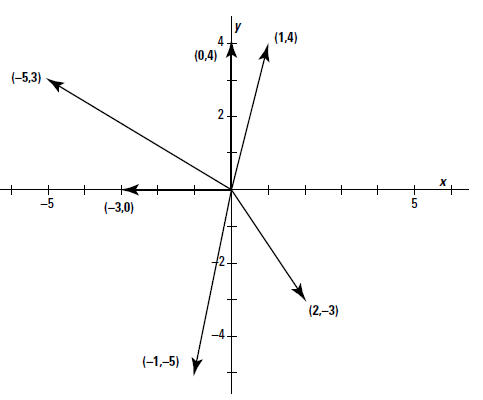
\includegraphics[scale=1]{imgs/Vektor1.png}\end{center}
\section{Darstellung von Vektoren im $\mathbb{R}^3$}
Vektoren im $\mathbb{R}^3$ bezeichnet man auch als dreidimensional.
\begin{equation*}
\vec{a} = \begin{pmatrix}x\\y\\z \end{pmatrix} \quad\quad \mbox{z.B.} \begin{pmatrix}2\\3\\4 \end{pmatrix}
\end{equation*}
\begin{center}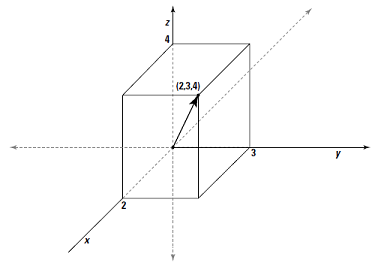
\includegraphics[scale=1]{imgs/Vektor3D.png}\end{center}
\section{Spezielle Vektoren}
\begin{mydef}
$\vec{0} = \begin{pmatrix}0\\0\\0 \end{pmatrix}$ heisst \textbf{Nullvektor}.\end{mydef}
\noindent Dargestellt wird der Nullvektor als Punkt. Der Nullvektor ist das neutrale Element der Addition:
\begin{equation*}
\vec{u} + \vec{0} = \vec{u} 
\end{equation*}
\begin{mydef}
$-\vec{a}$ ist der zu $\vec{a}$ \textbf{inverse Vektor}.\end{mydef}
\begin{equation*}
\vec{a} + -(\vec{a}) = \vec{0}
\end{equation*}
\subsection{Einheistvektor}
\begin{mydef}Ein \textbf{Einheitsvektor} (auch Basisvektor oder normierter Vektor) ist ein Vektor mit der Länge 1. \end{mydef}
\noindent Um aus einem beliebigen Vektor einen Vektor mit der selben Richtung, aber der Länge 1 zu erstellen - einen Vektor zu normalisieren - rechnet man
\begin{equation*} 
\vec{a}^0 = \frac{\vec{a}}{|\vec{a}|}
\end{equation*}
Ein Einheitsvektor wird aus einem Vektor, Bsp. $\vec{a}$ gebildet. Der Einheitsvektor von $\vec{a}$ hat dieselbe Richtung wie $\vec{a}$ aber die Länge 1. Anders gesagt, der Vektor wurde Normalisiert, also auf die Länge 1 gebracht.\\
\\
Der Einheitsvektor von $\vec{v} $ist $\vec{v}_0$ \\
\\
Die eigentliche Länge des Einheitsvektors ist laut Definition immer 1.\\
Die Formel zur Berechnung der Einheitsvektoren Werte für x,y und z lautet wie folgt. \\
\begin{equation*}
	\vec{v_0} =  \frac{\vec{v}}{|\vec{v}|} 
\end{equation*}

Ein Rechenbeispiel:\\
Gegeben ist der Vektor
\begin{eqnarray*}
	\vec{v} &=& \begin{pmatrix}8\\6\\1\end{pmatrix}\\
	\vec{v_0} &=& \frac{\begin{pmatrix}8\\6\\1\end{pmatrix}}{\sqrt{8^2+6^2+1}}
\end{eqnarray*}
Zuerst berechnen wir den Betrag des Vektors
\begin{equation*}
	|\vec{v}|= \sqrt{8^2+6^2+1}  = \sqrt{101} =10.04987
\end{equation*}
Danach werden die x, y und z Werte des Vektors durch den Betrag des Vektors gerechnet. Daraus ergeben sich die x, y und z Werte des Einheitsvektors $\vec{v_0}$

\begin{eqnarray*}
	8 / 10.04987 = 0.79603\\
	6 / 10.04987 = 0.59702\\
	1 / 10.04987 = 0.99503\\
	\vec{v_0} = \begin{pmatrix}0.79603\\0.59702\\0.99503\end{pmatrix}
\end{eqnarray*}

Wichtig
Der Einheitsvektor eines Nullvektors kann nicht ausgerechnet werden weil der Nullvektor hat keine definierte Richtung hat. Da der Betrag des Vektors gleich 0 ist, würde zudem während der Berechnung durch 0 geteilt, was selbstverständlich nicht erlaubt ist.

\section{Ortsvektoren}
\begin{mydef}Ein \textbf{Ortsvektor} ist ein Vektor, der vom Bezugspunkt (Ursprung $(0,0,0)$) zu einem Punkt zeigt.\end{mydef}
\begin{equation*}
A(3/5) \quad\quad\quad \vec{a} = \begin{pmatrix}3\\5 \end{pmatrix}
\end{equation*}
Herleitung: Punkte lassen sich ebenfalls mit den Komponenten $x$, $y$ und $z$ darstellen, z.B.
\begin{equation*}
A(x/y/z)\quad\quad \mbox{z.B.}\quad A(1/2/3)
\end{equation*}
Den Punkt A erreichen wir vom Koordinatenursprung, indem wir $1$ Einheit in die X, $2$ Einheiten in die Y und $3$ Einheiten in die Z Richtung gehen. Durch diese Bewegung ergibt sich der Ortsvektor
\begin{equation*}
\vec{a} = \begin{pmatrix}a_x\\a_y\\a_z\end{pmatrix} = \begin{pmatrix}1\\2\\3\end{pmatrix}
\end{equation*}
\begin{mydef}
Ein \textbf{Verbindungsvektor} verbindet zwei Punkte $A$ und $B$. \end{mydef}
\noindent Um zwei Punkt zu verbinden, gehen wir von Punkt $A$ zum Koordinatenursprung (dies entspricht dem negativen Ortsvektor $\vec{a}$) und von dort aus zum Punkt B über den Ortsvektor $\vec{b}$.
\begin{equation*}\vec{AB} = \vec{b} - \vec{a}\end{equation*}
\section{Vektorraum}
\begin{mydef}Ein \textbf{Vektorraum} ist eine algebraische Struktur, welche als Elemente Vektoren besitzt.\end{mydef}
Mit den Vektoren in einem Vektorraum müssen bestimmte Operationen möglich sein, beispielsweise die Addition und die Multiplikation mit einem Skalar. Als Ergebnis muss dabei wieder ein Vektor des selben Vektorraumes entstehen. Ausserdem müssen das Assoziativgesetz und Kommutativgesetz gelten und es braucht ein neutrales sowie ein inverses Element.
\begin{mydef}Die \textbf{Basis} eines Vektorraums ist die Menge von Vektoren, die es ermöglicht, jeden anderen Vektor als Linearkombination darzustellen.\end{mydef}
\begin{mydef}Die Anzahl Basisvektoren wird \textbf{Dimension} des Vektorraums genannt.\end{mydef}
\section{Gesetze und Rechenoperationen mit Vektoren}
\subsection{Addition}
Zwei Vektoren werden addiert, indem ihre Komponenten addiert werden. Es entsteht ein neuer Vektor.
\begin{equation*}
\begin{pmatrix}a_x\\a_y\\a_z\end{pmatrix} + \begin{pmatrix}b_x\\b_y\\b_z\end{pmatrix} = \begin{pmatrix}a_x + b_x\\a_y + b_y\\a_z + b_z\end{pmatrix}
\end{equation*}
\begin{myexample}
\begin{equation*}\begin{pmatrix}2\\4\end{pmatrix} + \begin{pmatrix}3\\1\end{pmatrix} = \begin{pmatrix}2+3\\4+1\end{pmatrix} = \begin{pmatrix}5\\5\end{pmatrix}\end{equation*}
\end{myexample}
\begin{center}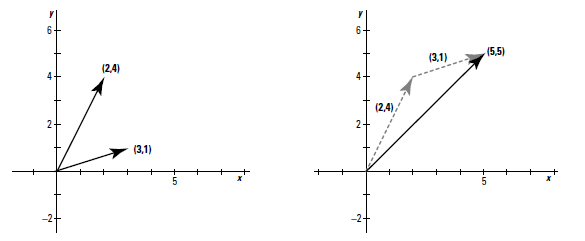
\includegraphics[scale=0.85]{imgs/VektorAddition.png}\end{center}
\subsection{Skalare Grösse}
In der Mathematik und in der Physik werden zwei Arten von Grössen unterschieden. Die Vektoriellen und die Skalaren.
Die Vektorielle Grösse sind richtungsabhängig und die Skalaren richtungsunabhängig. Als passendes Beispiel für eine vektorielle Grösse kann ein Vektor genannt werden. Er besitzt zwei Werte, in welche Richtung zeigt er und wie lang ist er. Eine Skalare Grösse hat dagegen nur einen bestimmten Wert.
Skalare Grössen sind:
\begin{itemize}
	\item Masse
	\item Temperatur
	\item Druck
	\item Dichte
\end{itemize}
\subsection{Multiplikation mit einem Skalar}
Wird ein Vektor mit einem Skalar (einer Zahl) multipliziert, wird der Vektor um diesen Faktor gestreckt/gestaucht. Die Zahl wird mit jeder Komponente des Vektors multipliziert:
\begin{equation*}
k \cdot \begin{pmatrix}v_x\\v_y\\v_z\end{pmatrix} = \begin{pmatrix}kv_x\\kv_y\\kv_z\end{pmatrix}
\end{equation*}
\begin{myexample}
\begin{equation*}
5\cdot \vec{a} = 3\cdot \begin{pmatrix}2\\4\end{pmatrix} = \begin{pmatrix}3\cdot 2\\ 3 \cdot 4\end{pmatrix} = \begin{pmatrix}6\\12 \end{pmatrix}
\end{equation*}
Grafisch:
\begin{center}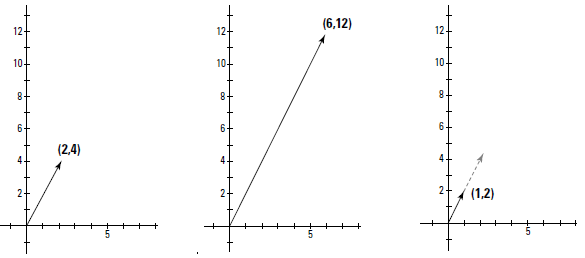
\includegraphics[scale=0.85]{imgs/VektorMultiplikation.png}\end{center}
\end{myexample}
\subsection{Wert eines Vektors}
Der Wert (auch Betrag oder Norm) eines Vektors ist seine Länge und wird wie folgt mit Hilfe des Satzes von Pythagoras berechnet:
\begin{equation*}
|\vec{a}| = \sqrt{a_{x}^{2} + a_{y}^{2} + a_{z}^{2}}
\end{equation*}
\begin{myexample}
\begin{equation*}
\vec{a} = \begin{pmatrix}1\\2\\3\end{pmatrix} \quad\quad\quad |\vec{a}| = \sqrt{1^2 + 2^2 + 3^2} = \sqrt{14}
\end{equation*}
\end{myexample}
\subsection{Skalarprodukt}
\begin{mydef}Das Skalarprodukt (auch inneres Produkt oder Punktprodukt) ist die mathematische Verknüpfung, die zwei Vektoren eine Zahl (Skalar) zuordnet.\end{mydef}
Mulitplikation von zwei Vektore, als Ergebniss erhalten wir ein Skalar / Zahl
\begin{equation*}
\vec{a} \cdot \vec{b} = \begin{pmatrix}a_x\\a_y\\a_z\end{pmatrix} \cdot \begin{pmatrix}b_x\\b_y\\b_z\end{pmatrix} = a_x \cdot b_x + a_y \cdot b_y + a_z \cdot b_z
\end{equation*}
Ausserdem gilt auch:
\begin{eqnarray*}
\vec{a} \cdot \vec{b} & =& |\vec{a}| \cdot |\vec{b}| \cdot \cos \measuredangle(\vec{a}, \vec{b})\\
\cos \measuredangle(\vec{a}, \vec{b}) &=& \frac{\vec{a} \cdot \vec{b} }{|\vec{a}| \cdot |\vec{b}|}
\end{eqnarray*}
Liegen die Vektoren also in einem Koordinatensystem, so können wir das Skalarprodukt ausrechnen. Mit der zweiten Formel können wir zudem den Winkel phi $\phi$ zwischen den beiden Vektoren ermitteln. Diese Formel lässt sich aus dem Cosinussatz herleiten.
\subsubsection{Eigenschaften des Skalarprodukts}
\begin{enumerate}
	\item $\vec{a} \cdot \vec{b} = \vec{b}\cdot \vec{a}$
	\item $\vec{a} \cdot (\vec{b}+\vec{c}) = \vec{a} \cdot \vec{b} + \vec{a} \cdot \vec{c}$
	\item $(\lambda \cdot \vec{a}) \cdot \vec{b} = \lambda \cdot (\vec{a} \cdot \vec{b}),  \lambda \in \mathbb{R}$
\end{enumerate}
\subsection{Orthogonalität}
\begin{mydef}Zwei Vektoren stehen senkrecht zueinander (sie sind orthogonal), wenn ihr Skalarprodukt 0 beträgt.\end{mydef}
\begin{equation*}\vec{a}\cdot \vec{b} = 0 \mbox{, wenn } \measuredangle (\vec{a};\vec{b})=90º\end{equation*}
\begin{center}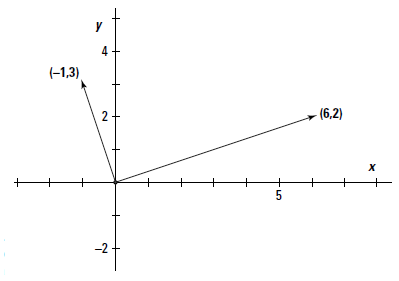
\includegraphics[scale=0.85]{imgs/Orthogonalitaet.png}\end{center}
\begin{equation*}
\vec{a} \cdot \vec{b} = (-1) \cdot 6 + 3 \cdot 2 = -6 + 6 = 0
\end{equation*}
\subsection{Betrag mit Hilfe des Skalarprodukts berechnen}
Berechnen wir das Skalarprodukt von ein und demselben Vektor, finden wir folgendes heraus:
\begin{eqnarray*}\vec{a}^2&=&\vec{a}\cdot \vec{a}\\
 &=& a_{1}^{2} + a_{2}^{2} + a_{3}^{2} \\
 &=& |\vec{a}|^2\end{eqnarray*}
Wir können also den Betrag eines Vektors mit Hilfe des Skalarprodukts berechnen. 
\section{Aufgaben}
\begin{enumerate}
	\item Gegeben sind |$\vec{a}|=3$, |$\vec{b}|=4$, $\measuredangle(a,b) = 60º$, $\vec{u}=2\vec{a}+\vec{b}$ und $\vec{v}=3\vec{a}-2\vec{b}$. Berechnen Sie das Skalarprodukt und den Winkel zwischen $\vec{u}$ und $\vec{v}$.\\\\
	Zuerst berechnen wir das Skalarprodukt von $\vec{a}$
	\begin{eqnarray*}
		  a^2 &=& \begin{pmatrix}a_1\\a_2\\a_3\end{pmatrix} \cdot \begin{pmatrix}a_1\\a_2\\a_3\end{pmatrix} \\
			&=& \sqrt{a_{1}^{2} + a_{2}^{2}+a_{3}^{2}}^2\\
			&=& |a|^2 = 4^2 = 16
	\end{eqnarray*}
	Nun das Skalarprodukt von $\vec{b}$:
	\begin{eqnarray*}
		b^2 &=& \begin{pmatrix}b_1\\b_2\\b_3\end{pmatrix} \cdot \begin{pmatrix}b_1\\b_2\\b_3\end{pmatrix}\\ 
		&=& \sqrt{b_{1}^{2} + b_{2}^{2}+b_{3}^{2}}^2\\
		&=& |b|^2 = 3^2 = 9
	\end{eqnarray*}
	Nun nun noch das Skalarprodukt zwischen $\vec{a}$ und $\vec{b}$:
	\begin{equation*}
		\vec{a}\cdot \vec{b} = |\vec{a}| \cdot |\vec{b}| \cdot \cos(60º) = 6
	\end{equation*}
	Nun berechnen wir den Winkel:
	\begin{eqnarray*}
	\cos(\measuredangle (u,v)) &=& \frac{\vec{u}\cdot \vec{v}}{|\vec{u}|\cdot |\vec{v}|}\\
	&=&\frac{(2\vec{a}+\vec{b})\cdot (3\vec{}-2\vec{b})}{|2\vec{a} + \vec{b}| \cdot |3\vec{a}-2\vec{b}|} \\
	&=& \frac{6\vec{a}^2 - \vec{a}\vec{b}-2\vec{b}^2}{|2\vec{a} + \vec{b}| \cdot |3\vec{a}-2\vec{b}|}\\
	&=& \frac{6\cdot 16 - 6 - 2\cdot 9}{\sqrt{(2\vec{a} + \vec{b})^2}\cdot \sqrt{(3\vec{a}-2\vec{b})^2}}\\
	&=& \frac{72}{\sqrt{4\vec{a}^2+4\vec{a}\cdot\vec{b}+\vec{b}^2}\cdot\sqrt{9\vec{a}^2 - 12\vec{a}\vec{b}+4\vec{b}^2}}\\
	&=&\frac{72}{\sqrt{4\cdot 16 + 4 \cdot 6 + 9}\cdot\sqrt{9\cdot 16 - 12\cdot 6 + 4\cdot 9}}\\
	&=&\frac{72}{\sqrt{97}\cdot\sqrt{108}}\\
	\end{eqnarray*}
	Somit ist der Winkel $45.29º$ und das Skalarprodukt $\vec{u}\vec{v} = 72$.
\end{enumerate}
\newpage

\section{Geschlossene Vektorkette}
Eine geschlossene Vektorenkette sind aneinandergelegte Vektoren (Addition von mehreren Vektoren) die wieder zum Ausgangspunkt zurückführen. Die Summe aller Vektoren ist der Nullvektor, es findet also keine Verschiebung statt.

\section{Verschiebevektor}
Verschiebungsvektor
Ein Verschiebungsvektor beschreibt die Verschiebung/Translation resp. das Abbilden von einem Punkt auf einen Anderen.
Ein Beispiel:
Folgende Punkte sind gegeben:
\begin{eqnarray*}
	A(2/3)\\
	B(1/5)
\end{eqnarray*}
Nun gilt es zu bestimmen, welcher Vektor (Verschiebungsvektor), den Punkt A auf den Punkt B abbildet.\\
Dazu Subtrahieren wir die x und y Werte des Urbildpunktes A von den Werten des Bildpunktes B.
Es ergibt sich der Verschiebungsvektor  $\vec{AB}$.\\
\begin{equation*}
	\vec{AB} =  \begin{pmatrix}1-2\\5-3\end{pmatrix} = \begin{pmatrix}-1\\2\end{pmatrix} 
\end{equation*}

\section{Linearkombination}
Unter einer Linearkombination von Vektoren versteht man eine Summe von Vektoren (Vektoraddition), wobei jeder Vektor noch mit einer reelen Zahl multipliziert wird. Als Ergebnis erhält man wieder einen Vektor
\begin{equation*}
\vec{v} = \lambda_1 \cdot \vec{a_1} + \lambda_2 \cdot \vec{a_2} + ... + \lambda_n \cdot \vec{a_n}
\end{equation*}
Dabei ist $\vec{v}$ der Ergebnisvektor und $\vec{a_1}$, $\vec{a_2}$,...,$\vec{a_n}$ sind die Vektoren, die jeweils mit einer reelen Zahl $\lambda_1, \lambda_2,...,\lambda_n$ multipliziert und anschliessend addiert werden.\\\\
Beispiel: Gegeben sind die beiden Vektoren
\begin{equation*}
\vec{a_1} = \begin{pmatrix}1\\3\end{pmatrix} \quad\quad\quad \vec{a_2} = \begin{pmatrix}3\\0\end{pmatrix}
\end{equation*}
Finde zwei Linearkombinationen der beiden Vektoren
\begin{equation*}
\vec{v_1} = 2\cdot \vec{a_1} + 3\cdot \vec{a_2}=2\cdot \begin{pmatrix}1\\3\end{pmatrix} + 3 \cdot \begin{pmatrix}3\\0\end{pmatrix} = \begin{pmatrix}11\\6\end{pmatrix}
\end{equation*}
\begin{equation*}
\vec{v_2} = 3\cdot \vec{a_1} - 1\cdot \vec{a_2}=3\cdot \begin{pmatrix}1\\3\end{pmatrix} - 1 \cdot \begin{pmatrix}3\\0\end{pmatrix} = \begin{pmatrix}0\\9\end{pmatrix}
\end{equation*}
Betrachten wir nun folgende Linearkombination grafisch:
\begin{equation*}
\vec{v} = 1\cdot \vec{a_1} + 0.5\cdot \vec{a_2}=1\cdot \begin{pmatrix}1\\3\end{pmatrix} + 0.5 \cdot \begin{pmatrix}3\\0\end{pmatrix} = \begin{pmatrix}2.5\\3\end{pmatrix}
\end{equation*}
\begin{center}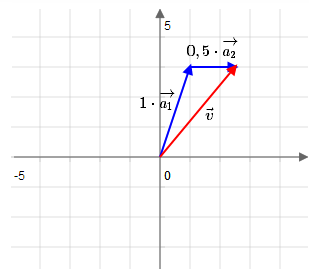
\includegraphics[scale=1.1]{imgs/Linearkombination1.png}\end{center}
\section{Lineare Abhängigkeit bzw. Unabhängigkeit}
Haben zwei Vektoren die gleiche Richtung - sie sind kolinear - so sind sie linear abhängig.
\begin{center}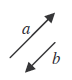
\includegraphics[scale=0.9]{imgs/pic2.png}\end{center}
\begin{mydef}
Eine Menge von Vektoren heisst linear abhängig, wenn sich mindestens einer davon als Linearkombination der anderen darstellen lässt:
\begin{equation*}
c=\lambda_1 \cdot \vec{a} + \lambda_2 \cdot \vec{b}
\end{equation*}
\end{mydef}
\noindent In der Regel ist vorher allerdings nicht bekannt, welcher der Vektoren sich als Linearkombination der anderen darstellen lässt, deshalb wird eine allgemeine Gleichung eingeführt, deren Lösungsmenge zu bestimmen ist:
\begin{equation*}
\lambda_1 \cdot \vec{a_1} + \lambda_2 \cdot \vec{b} + \lambda_3 \cdot \vec{c} = \vec{0}
\end{equation*}
\subsection{Lineare Abhängigkeit von 2 Vektoren}
Zwei Vektoren heissen linear abhängig, wenn es zwei Zahlen $\lambda_1$ und $\lambda_2$ gibt, die nicht beide Null sind, so dass gilt
\begin{equation*}
\lambda_1 \cdot \vec{a} + \lambda_2 \cdot \vec{b} = \vec{0}
\end{equation*}
Anders formuliert: 
Zwei Vektoren sind genau dann linear abhängig, wenn sich der Nullvektor durch eine Linearkombination der beiden Vektoren erzeugen lässt.\\\\
\subsection{Lineare Abhängigkeit im $\mathbb{R}^2$}
Beispiel: Gegeben sind die beiden Vektoren $\vec{a}$ und $\vec{b}$
\begin{equation*}
\vec{a} = \begin{pmatrix}1\\2\end{pmatrix} \quad\quad\quad \vec{b} = \begin{pmatrix}2\\4\end{pmatrix}
\end{equation*}
Zwei Vektoren sind genau dann linear abhängig, wenn sie Vielfache voneinander sind:
\begin{eqnarray*}
\vec{a} &=& \lambda \cdot \vec{b}\\
\begin{pmatrix}1\\2\end{pmatrix} &=& \lambda \cdot \begin{pmatrix}2\\4\end{pmatrix}
\end{eqnarray*}
Wenn es nun ein $\lambda$ ungleich Null gibt, das das Gleichungssystem löst, so sind die Vektoren linear abhängig.
\begin{eqnarray*}
1=\lambda \cdot 2 \quad &\to&\quad \lambda = 0.5\\
2=\lambda \cdot 4 \quad &\to&\quad \lambda = 0.5
\end{eqnarray*}
Alternativ können wir die Determinante untersuchen, die sich aus den zwei Vektoren ergibt. Ist diese gleich Null, so sind die Vektoren linear abhängig
\begin{equation*}
|D| = \begin{vmatrix}1\quad 2\\2\quad 4\end{vmatrix} = 0
\end{equation*}
\subsection{Eigenschaften von Vektoren im $\mathbb{R}^2$}
\begin{itemize}
	\item 2 Vektoren sind im $\mathbb{R}^2$ genau dann linear abhängig, wenn sie parallel sind.
	\item 3 (oder mehr) Vektoren sind im $\mathbb{R}^2$ stets linear abhängig.
\end{itemize}
Erklärung: Der $\mathbb{R}^2$ ist definiert als ein Vektorraum, der durch 2 linear unabhängige Vektoren $\vec{a}$ und $\vec{b}$ aufgespannt wird. Diese zwei Vektoren nennt man Basis des Vektorraums. Meist verwendet man die sog. Standardbasis (kanonische Basis):
\begin{equation*}
e_1 = \begin{pmatrix}1\\0\end{pmatrix}\quad\quad e_1 = \begin{pmatrix}0\\1\end{pmatrix}
\end{equation*}
Mit Hilfe dieser Basisvektoren kann jeder beliebige Vektor des $\mathbb{R}^2$ als Linearkombination geschrieben werden, z.B.:
\begin{equation*}
2\cdot \begin{pmatrix}1\\0\end{pmatrix} + 3\cdot \begin{pmatrix}0\\1\end{pmatrix} = \begin{pmatrix}2\\3\end{pmatrix}
\end{equation*}
Es geling also nicht, uns einen dritten Vektor auszudenken, der nicht als Basis der beiden Basisvektoren geschrieben werden könnte. Daraus folgt, dass 3 (oder mehr) Vektoren im $\mathbb{R}^2$ stets linear abhängig sind.
\subsection{Lineare Abhängigkeit von 3 Vektoren}
Drei Vektoren heissen linear abhängig, wenn es drei Zahlen $\lambda_1, \lambda_2$ und $\lambda_3$ gibt, die nicht alle gleich Null sind, so dass gilt
\begin{equation*}
\lambda_1 \cdot \vec{a_1} + \lambda_2 \cdot \vec{a_2} + \lambda_3 \cdot \vec{a_3} = 0 
\end{equation*}
\subsection{Lineare Abhängigkeit im $\mathbb{R}^3$}
Gegeben sind die drei Vektoren:
\begin{equation*}
\vec{a} = \begin{pmatrix}1\\1\\2\end{pmatrix}\quad\quad \vec{b} = \begin{pmatrix}3\\-1\\1\end{pmatrix}\quad\quad \vec{c} = \begin{pmatrix}-1\\3\\3\end{pmatrix}
\end{equation*}
Drei Vektoren im $\mathbb{R}^3$ sind genau dann linear abhängig, wenn sie in einer Ebene liegen. 
\begin{center}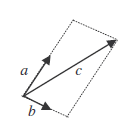
\includegraphics[scale=0.9]{imgs/pic1.png}\end{center}
Das ist dann der Fall, wenn sich der dritte Vektor durch die beiden anderen ausdrücken lässt. Es entsteht das folgende Gleichungssystem:
\begin{eqnarray*}
\lambda_1 + 3\cdot \lambda_2 &=& -1\\
\lambda_1 - \lambda_2 &=& 3\\
2\cdot \lambda_1 + \lambda_2 &=& 3
\end{eqnarray*}
Lassen sich die Unbekannten $\lambda_1$ und $\lambda_2$ eindeutig berechnen, ohne dass $\lambda_1 = \lambda_2 = 0$ gilt, sind die Vektoren linear abhängig.\\\\
Alternativ lässt sich wiederum die Determinante berechnen. Ist diese gleich Null, so sind die Vektoren linear abhängig.
\subsection{Eigenschaften von Vektoren im $\mathbb{R}^3$}
\begin{itemize}
	\item 2 Vektoren sind im $\mathbb{R}^3$ genau dann linear abhängig, wenn sie parallel sind.
	\item 3 Vektoren sind im $\mathbb{R}^3$ genau dann linear abhängig, wenn sie in einer Ebene liegen.
	\item 4 (oder mehr) Vektoren sind im $\mathbb{R}^3$ stets linear abhängig (selbe Erklärung wie im $\mathbb{R}^2$)
\end{itemize}

\newpage
\section{Vektorprodukt}
\begin{center}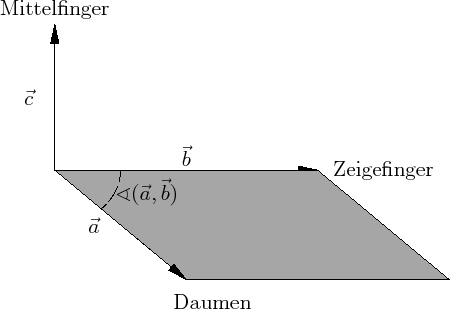
\includegraphics[scale=0.7]{imgs/Vektorprodukt.png}\end{center}
Wir suchen $\vec{c}$, so dass $\vec{c} \perp \vec{a}$ und $\vec{c} \perp \vec{b}$, wenn \\
\begin{eqnarray*}
	\vec{a} = \begin{pmatrix}a_1\\a_2\\a_3\end{pmatrix}\\ 
	\vec{b} = \begin{pmatrix}b_1\\b_2\\b_3\end{pmatrix}
\end{eqnarray*}
ist.\\
\\
Es muss 
\begin{equation*}
	\vec{a}* \vec{c} = 0 \land \vec{b} * \vec{c} = 0
\end{equation*}
sein.\\
Ist 
\begin{equation*}\vec{c} = \begin{pmatrix}x\\y\\z\end{pmatrix}\end{equation*}
so muss also
\begin{eqnarray*}
	\begin{vmatrix} a_1x + a_2y + a_3z &=& 0 \\ 
	b_1x+b_2y+b_3z &=& 0 \end{vmatrix}
\end{eqnarray*}
Wir haben also 2 Gleichungen, aber 3 Variabeln $\to$ Eine Variebel ist frei wählbar\\
Ein Beispiel:
\begin{eqnarray*}
	\begin{vmatrix}4x + 5y + z &=& 1 \\ 
	2x-y+2z &=& 0 \end{vmatrix}
\end{eqnarray*}
Wir nehmen an $z = 1$
\begin{eqnarray*}
	\begin{vmatrix}4x + 5y &=& 0 \\ 
	2x-y &=& -2 \end{vmatrix}\\
	\begin{vmatrix}4x + 5y &=& 0 \\ 
	4x-2y &=& -4 \end{vmatrix}\\
	\begin{vmatrix}4x  &=& -5y \\ 
	4x&=& -4 + 2y\end{vmatrix}
\end{eqnarray*}
Wir setzn die beiden Gleichungen eineander Gleich und erhalten für y:
\begin{eqnarray*}
	7y = 4\\
	y = \frac{4}{7}
\end{eqnarray*}
Wir setzen y ein in:
\begin{eqnarray*}
	14x = -10\\
	x = -\frac{10}{14}\\
	x = -\frac{5}{7}
\end{eqnarray*}
Eine Lösung lautete also
\begin{equation*}(-\frac{5}{7} / \frac{4}{7} / 1)\end{equation*}
Dann finden wir weitere Lösungen mit 
\begin{equation*}z=2, z=3,z=4 \ldots\end{equation*}
Also berechen wir x und y in Abhängigkeit von z\\
somit müssen wir 
\begin{eqnarray*}
	\begin{vmatrix}a_1x + a_2y &=& - a_3z\\ 
	b_1x+b2_y &=& -b_3z\end{vmatrix}\\
\end{eqnarray*}
lösen\\
\\
Mit der Cramerschen Regel finden wir\\
\begin{eqnarray*}
D &=& a_1b_2-a_2b_1 \\
\\
D_x &= &\begin{vmatrix}-3a_z &  a_2 \\ 
	-b_3z & b_2 \end{vmatrix} \\
&=& -a_3b_2z + a_2b_3z \\
&=& z(a_2b_3 -a_3b_2)\\
\\
D_y &= &\begin{vmatrix}a_1 &  -a_3z \\ 
	b_1 & -b_3z \end{vmatrix} \\
&=& -a_1b_3z + a_3b_1z \\
&=& z(a_3b_1 -a_1b_3)\\
\end{eqnarray*}
Somit
\begin{eqnarray*}
	x = \frac{z(a_2b_3-a_3b_2)}{a_1b_2-a_2b_1}, y = \frac{z(a_3b_1-a_1b_3)}{a_1b_2 -a_2b_1}
\end{eqnarray*}
z ist frei wählbar.\\
Damit wir die Brüche auflösen können, wählen wir z = Nenner, damit wird
\begin{eqnarray*}
	x = a_2b_3 - a_3b_2\\
	y = a_3b_1 - a_1b_3 \\
	z = a_1b_2 - a_2b_1\\
\end{eqnarray*}

\begin{mydef}
	Ist
	\begin{equation*} \vec{a} = \begin{pmatrix}a_1 \\ a_2 \\ a_3\end{pmatrix},  \vec{b} = 					\begin{pmatrix}b_1 \\ b_2 \\ b_3\end{pmatrix} \end{equation*}
	So heisst
	\begin{equation*} \vec{a} \times \vec{b} := \begin{pmatrix}a_2b_3 -a_3b_2 \\ a_3b_1 - a_1b_3 \\ a_1b_2 - a_2b_1\end{pmatrix} \end{equation*}
	''a kreuzt b''\\
	\underline{das Vektorprodukt/ Kreuzprodukt von $\vec{a}$ und $\vec{b}$}
\end{mydef}
\noindent 
Beim Skalarprodukt erhalten wir als Ergebnis einen Skalar, beim Vektorprodukt einen Vektor. \\
\\
Jede Komponente (x,y,z) lässt sich als Determinante darstellen
\begin{eqnarray*}
	\vec{a} \times \vec{b} &=& 
	\begin{pmatrix}
		&
		\begin{vmatrix}
			a_2 & b_2\\
			a_3 & b_3
		\end{vmatrix}
		&
		\\
		\\
		&
		\begin{vmatrix}
			a_3 & b_3\\
			a_1 & b_1
		\end{vmatrix}
		&
		\\
		\\
		&
		\begin{vmatrix}
			a_1 & b_1\\
			a_2 & b_2
		\end{vmatrix}
		&
	\end{pmatrix} 
\end{eqnarray*}

\begin{myexample}
	\begin{eqnarray*}
		\vec{a} = \begin{pmatrix}2\\ 1\\ 0 \end{pmatrix}, \vec{b} = \begin{pmatrix}3\\ -1\\ 1 \end{pmatrix}\\
		\vec{a} \times \vec{b} = \begin{pmatrix} 1*1 &-& 0(-1) \\ 0* 3 &-&2 * 1 \\ 2 * (-1) &-& 1 * (-1)\end{pmatrix} = \begin{pmatrix}1 \\ -2 \\ -1 \end{pmatrix}
	\end{eqnarray*}
\end{myexample}
 \newpage
 \noindent
 Wir erinnern uns, dass wir jeden Vektor als Linearkombination darstellen können
 \begin{eqnarray*}
 \vec{a} &=& \begin{pmatrix}a_1\\a_2\\a_3\end{pmatrix} \leftrightarrow \vec{a} = a_1\vec{e_a} + a_2\vec{e_2}+a_3\vec{e_3}\\
 \shortintertext{also}
 \vec{a} \times \vec{b} &=& (a_2b_3-a_3b_2)\vec{e_1} + (a_3b_1-a_1b_3)\vec{e_2}+(a_1b_2-a_2b_1)\vec{e_3}\\
 &=&  a_2b_3\vec{e_1}+a_3b_1\vec{e_2}+a_1b_2\vec{e_3}-a_3b_2\vec{e_1} - a_1b_3\vec{e_2} - a_2b_1\vec{e_3}
 \end{eqnarray*}
 Ein Term mit 3 positiven und 3 negativen Produkten, die je aus 3 Faktoren bestehen.\\
 Dies ist eine dreireihige Determinante.
 \begin{eqnarray*}
 	\vec{a} \times \vec{b} =
 	\begin{vmatrix}
 		a_1 & b_1 & e_1\\
 		a_2 & b_2 & e_2\\
 		a_3 & b_3 & e_3\\
 	\end{vmatrix}
 \end{eqnarray*}
 \begin{myexample}
 	\begin{eqnarray*}
 		&\vec{a} = \begin{pmatrix}2 \\ 4 \\-1\end{pmatrix}, \vec{b} = \begin{pmatrix}1\\ 3 \\3\end{pmatrix}\\
 		\\
 		&\text{Regel von Sarrus anwenden}\\
 		&
 		\begin{tikzpicture}[>=stealth]
   			 \matrix [%
   			   matrix of math nodes,
   			   column sep=1em,
   			   row sep=1em
  			  ] (sarrus) {%
    			  2 & 1 & e_1 & 2 & 1 \\
   			  4 & 3 & e_2 & 4 & 3 \\
  			  -1 & 3 & e_3 & -1 & 3 \\
  			  };

    			\path ($(sarrus-1-1.north west)-(0.5em,0)$) edge ($(sarrus-3-1.south west)-(0.5em,0)$)
     			 	($(sarrus-1-3.north east)+(0.5em,0)$) edge ($(sarrus-3-3.south east)+(0.5em,0)$)
     			     	(sarrus-1-1)                          edge            (sarrus-2-2)
 				(sarrus-2-2)                          edge[->]        (sarrus-3-3)
  			     	(sarrus-1-2)                          edge            (sarrus-2-3)
    			     	(sarrus-2-3)                          edge[->]        (sarrus-3-4)
    			     	(sarrus-1-3)                          edge            (sarrus-2-4)
     			     	(sarrus-2-4)                          edge[->]        (sarrus-3-5)
   			     	(sarrus-3-1)                          edge[dashed]    (sarrus-2-2)
     			     	(sarrus-2-2)                          edge[->,dashed] (sarrus-1-3)
     			     	(sarrus-3-2)                          edge[dashed]    (sarrus-2-3)
     			     	(sarrus-2-3)                          edge[->,dashed] (sarrus-1-4)
   		             	(sarrus-3-3)                          edge[dashed]    (sarrus-2-4)
    			     	(sarrus-2-4)                          edge[->,dashed] (sarrus-1-5);

   			 \foreach \c in {1,2,3} {\node[anchor=south] at (sarrus-1-\c.north) {$+$};};
    			\foreach \c in {1,2,3} {\node[anchor=north] at (sarrus-3-\c.south) {$-$};};
 		\end{tikzpicture}\\
 		=& 6\vec{e_3}-\vec{e_2}+12\vec{e_1}-4\vec{e_3}-6\vec{e_2}+3\vec{e_1}\\
 		=& 15\vec{e_1}-7\vec{e_2}+ 2\vec{e_3}\\
 		= &\begin{pmatrix}15 \\ -7 \\ 2\end{pmatrix}
 	\end{eqnarray*}
 \end{myexample}
 \newpage
 \subsection{Vektorprodukt Richtung}
 Welche Richtung hat nun $\vec{a} \times \vec{b}$?\\
 Es gibt 2 Möglichkeiten:\\
\begin{center}
	 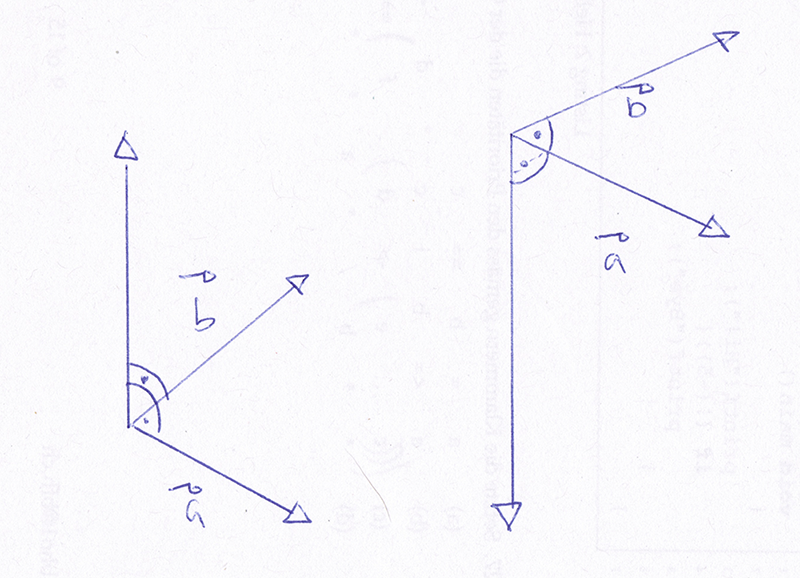
\includegraphics[width=0.8\textwidth]{imgs/richtung_kreuzprodukt.png}
 \end{center}
 \noindent
 Zum überprüfen, wählen wir $\vec{e_1}$ und $\vec{e_2}$ und untersuchen, ob $\vec{e_3}$ oder $-\vec{e_3}$ entsteht
 
 \begin{eqnarray*}
 	&\vec{e_1} \times \vec{e_2} = \\
 	&\begin{tikzpicture}[>=stealth]
   		 \matrix [%
   		   matrix of math nodes,
   		   column sep=1em,
   		   row sep=1em
  		  ] (sarrus) {%
    		  1 & 0 & e_1 & 1 & 0\\
   		  0 & 1 & e_2 & 0 & 1\\
  		  0 & 0 & e_3 & 0 & 0 \\
  		  };
    		\path ($(sarrus-1-1.north west)-(0.5em,0)$) edge ($(sarrus-3-1.south west)-(0.5em,0)$)
     		 	($(sarrus-1-3.north east)+(0.5em,0)$) edge ($(sarrus-3-3.south east)+(0.5em,0)$)
     		     	(sarrus-1-1)                          edge            (sarrus-2-2)
 			(sarrus-2-2)                          edge[->]        (sarrus-3-3)
  		     	(sarrus-1-2)                          edge            (sarrus-2-3)
    		     	(sarrus-2-3)                          edge[->]        (sarrus-3-4)
    		     	(sarrus-1-3)                          edge            (sarrus-2-4)
     		     	(sarrus-2-4)                          edge[->]        (sarrus-3-5)
   		     	(sarrus-3-1)                          edge[dashed]    (sarrus-2-2)
     		     	(sarrus-2-2)                          edge[->,dashed] (sarrus-1-3)
     		     	(sarrus-3-2)                          edge[dashed]    (sarrus-2-3)
     		     	(sarrus-2-3)                          edge[->,dashed] (sarrus-1-4)
   	             	(sarrus-3-3)                          edge[dashed]    (sarrus-2-4)
    		     	(sarrus-2-4)                          edge[->,dashed] (sarrus-1-5);

   		 \foreach \c in {1,2,3} {\node[anchor=south] at (sarrus-1-\c.north) {$+$};};
    		\foreach \c in {1,2,3} {\node[anchor=north] at (sarrus-3-\c.south) {$-$};};
 	\end{tikzpicture}\\
 	&= \vec{e_3}
 \end{eqnarray*}
\begin{center}
	 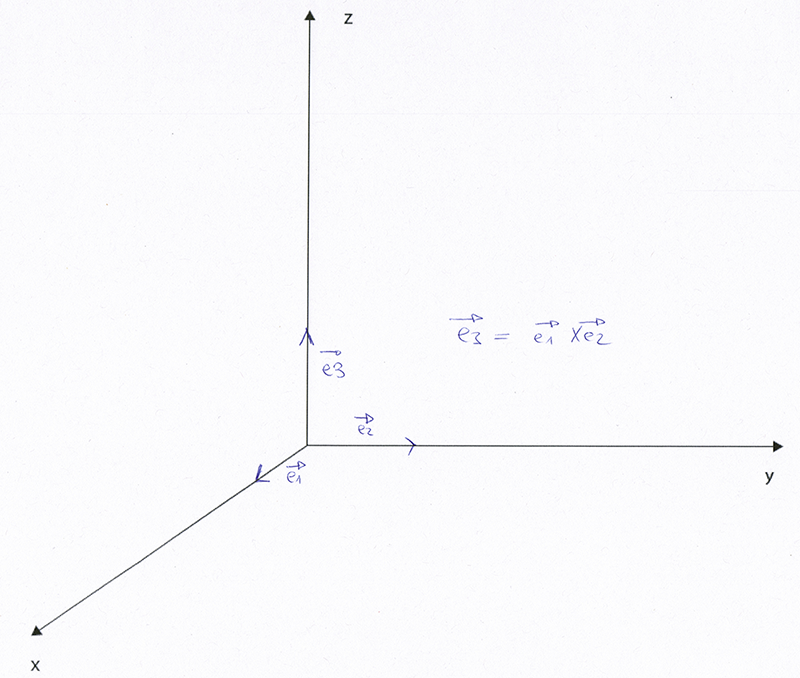
\includegraphics[width=0.8\textwidth]{imgs/rechtssystem.png}
 \end{center}
 Die Vektoren $\vec{a}$, $\vec{b}$ und $\vec{a} \times \vec{b}$ bilden \underline{in dieser Reihenfolge} ein Rechtssystem.\\
\begin{center}
	 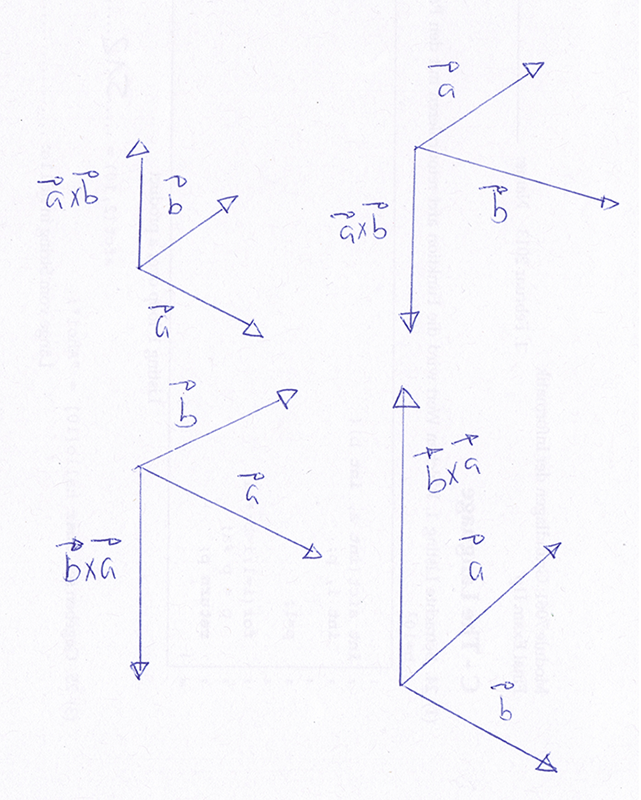
\includegraphics[width=0.8\textwidth]{imgs/rechtssystem_reihenfolge.png}
 \end{center}
 also $\vec{a} \times \vec{b} = -(\vec{b} \times \vec{a})$\\
 Das Kreuzprodukt ist nicht kommutativ.
 \newpage
 \subsection{Vektorprodukt Betrag}
 Welchen Betrag hat nun $\vec{a} \times \vec{b}$\\
Es ist $|\vec{a} \times \vec{b}|$ der \underline{Flächeninhalt} der von $\vec{a}$ und $\vec{b}$ aufgespannten \underline{Parallelogramms}.
 \begin{center}
	 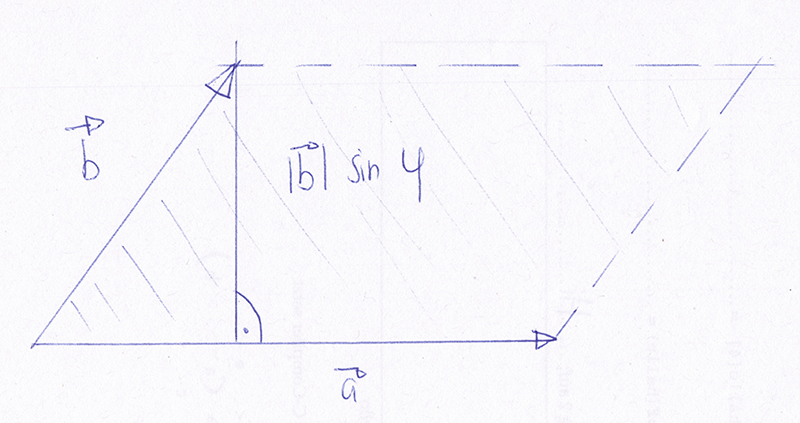
\includegraphics[width=0.8\textwidth]{imgs/kreuzprodukt_flaecheninhalt.png}
 \end{center}
\begin{myexample}
	Welche Oberfläche besitzt der Tetraeder ABDC, wenn A($\sqrt{2}$/0/0), B(0/$2\sqrt{2}$/0), C(0/0/$3\sqrt{2}$)und D(0/0/0)?
\begin{center}
	 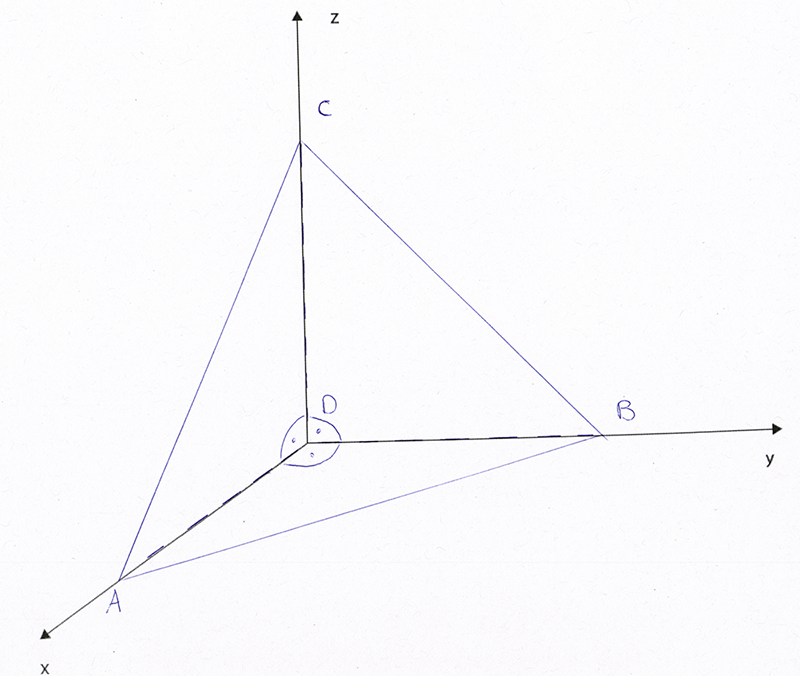
\includegraphics[width=0.8\textwidth]{imgs/tetraeder.png}
 \end{center}
\begin{eqnarray*}
	O &=& F(\triangle ABC) + F(\triangle ADB) + F(\triangle DBC) + F(\triangle ABC)\\
\shortintertext{wobei}
	F(\triangle ADC) &=& \frac{\sqrt{2} * 3\sqrt{2}}{2} = 3\\
	F(\triangle ADB) &=& \frac{\sqrt{2} * 2\sqrt{2}}{2} = 2\\
	F(\triangle DBC) &=& \frac{2\sqrt{2} * 3\sqrt{2}}{2} = 6\\
	F(\triangle ABC) &=& |\vec{AC} \times \vec{AB} | * \frac{1}{2}\\
	\vec{AC} &=& \vec{c} - \vec{a} = \begin{pmatrix}0\\0\\3 \sqrt{2}\end{pmatrix} - \begin{pmatrix}\sqrt{2}\\0\\0\end{pmatrix} = \begin{pmatrix}-\sqrt{2}\\0\\3\sqrt{2}\end{pmatrix}\\
	\vec{AB} &=& \vec{b} - \vec{a} = \begin{pmatrix}-\sqrt{2}\\2\sqrt{2}\\0\end{pmatrix}
\shortintertext{wird}
	\vec{AC} \times \vec{AB} & =&\\
	&&\begin{tikzpicture}[>=stealth]
   		 \matrix [%
   		   matrix of math nodes,
   		   column sep=1em,
   		   row sep=1em
  		  ] (sarrus) {%
    		  -\sqrt{2} &  -\sqrt{2} & e_1 &  -\sqrt{2} &  -\sqrt{2}\\
   		  0 & 2\sqrt{2} &  e_2& 0 & 2\sqrt{2}\\
  		  3\sqrt{2} & 0 & e_3 &  3\sqrt{2} & 0 \\
  		  };
    		\path ($(sarrus-1-1.north west)-(0.5em,0)$) edge ($(sarrus-3-1.south west)-(0.5em,0)$)
     		 	($(sarrus-1-3.north east)+(0.5em,0)$) edge ($(sarrus-3-3.south east)+(0.5em,0)$)
     		     	(sarrus-1-1)                          edge            (sarrus-2-2)
 			(sarrus-2-2)                          edge[->]        (sarrus-3-3)
  		     	(sarrus-1-2)                          edge            (sarrus-2-3)
    		     	(sarrus-2-3)                          edge[->]        (sarrus-3-4)
    		     	(sarrus-1-3)                          edge            (sarrus-2-4)
     		     	(sarrus-2-4)                          edge[->]        (sarrus-3-5)
   		     	(sarrus-3-1)                          edge[dashed]    (sarrus-2-2)
     		     	(sarrus-2-2)                          edge[->,dashed] (sarrus-1-3)
     		     	(sarrus-3-2)                          edge[dashed]    (sarrus-2-3)
     		     	(sarrus-2-3)                          edge[->,dashed] (sarrus-1-4)
   	             	(sarrus-3-3)                          edge[dashed]    (sarrus-2-4)
    		     	(sarrus-2-4)                          edge[->,dashed] (sarrus-1-5);

   		 \foreach \c in {1,2,3} {\node[anchor=south] at (sarrus-1-\c.north) {$+$};};
    		\foreach \c in {1,2,3} {\node[anchor=north] at (sarrus-3-\c.south) {$-$};};
 	\end{tikzpicture}\\
 	& =& 4\vec{e_3} - 6 \vec{e_2} - 12\vec{e_1} = \begin{pmatrix}-12\\-6 \\-4\end{pmatrix}\\
\shortintertext{und so}
	|\vec{AC}\times \vec{AB}| &=& \sqrt{144+36+16} = \sqrt{196} = 14\\
	F(\triangle ADC) &=& |\vec{AC}\times \vec{AB}| / 2 = 14 / 2 = 7
\shortintertext{Alle Flächen zusammenzählen}
	O &=& 3+2+6+7 = \underline{\underline{18}}
\end{eqnarray*}
\end{myexample}
\newpage

%-------------- Lineare Gleichungssysteme --------------

\chapter{Lineare Gleichungssysteme}
\section{Additionsmethode}
Beim Lösen eines Gleichungssystemes, versucht man herauszufinden, ob die einzelnen Gleichungen des Systems gemeinsame Lösungen besitzen. 
\begin{eqnarray*}
\begin{vmatrix} 4x + 3y &=& 10 \\ -5y &=& 2x - 19\end{vmatrix}
\end{eqnarray*}
Wir formen die Gleichungen so um, dass alle Variablen auf einer Seite stehen.
\begin{eqnarray*}
\begin{vmatrix} 4x + 3y &=& 10 \\ -2x -5y &=& - 19\end{vmatrix}
\end{eqnarray*}
Nun multiplizieren wir die zweite Gleichung mit 2, damit wir bei einer der beiden Unbekannten entweder den selben Koeffizienten oder das additiv inverse Element als Koeffizienten erhalten.
\begin{eqnarray*}
\begin{vmatrix} 4x + 3y &=& 10 \\ -4x -10y &=& - 38\end{vmatrix}
\end{eqnarray*}
Jetzt addieren wir die beiden Gleichungen miteinander und können anschliessend die Lösung für y bestimmen:
\begin{eqnarray*}
0x - 7y &=& -28\\
-7y &=& -28 \quad|: (-7)\\
y = 4
\end{eqnarray*}
Diesen Wert setzen wir nun in eine der ursprünglichen Gleichungen ein und lösen sie nach x auf:
\begin{eqnarray*}
4x+3y &=& 10\\
4x + 3 \cdot 4 &=& 10\\
4x + 12 &=& 10 \quad| -12\\
4x &=& -2 \quad |:4\\
x &=& -0.5
\end{eqnarray*}
Um y zu erhalten muss x in eine der Terme eingesetzt werden
\section{Cramersche Regel}
Wie lösen wir ein lineares Gleichungssystem
\begin{eqnarray*}
	\begin{vmatrix}a_1x + a_2y &=& c_1\\ 
	b_1x+b_2y &=& c_2\end{vmatrix}\\
\end{eqnarray*}
mit unbekannten Parameter?\\
Mulitplikation mit $b_1$ sowie $a_1$\\
Mit 
\begin{eqnarray*}
	a_1b_1x+a_2b_1y = c_1b_1\\
	-a_1b_1x -a_1b_2y = - c_2a_1
\end{eqnarray*}
Wird 
\begin{eqnarray*}
	a_2b_1y -a_1b_2y = b_1c_1-a_1c_2\\
	y(a_2b_1 -a_1b_2)= b_1c_1-a_1c_2\\
	\\
	y = \frac{b_1c_1-a_1c_2}{a_2b_1 -a_1b_2}
\end{eqnarray*}
Und mit 
Mulitplikation mit $b_2$ sowie $a_2$\\
\begin{eqnarray*}
	a_1b_2x+a_2b_2y = b_2c_2\\
	-a_2b_1x -a_2b_2y = - a_2c_2
\end{eqnarray*}
Wird
\begin{eqnarray*}
	a_1b_2x -a_2b_1x = b_2c_1-a_2c_2\\
	x(a_1b_2 -a_2b_1) = b_2c_1-a_2c_2\\
	x = \frac{b_2c_1-a_2c_2}{a_1b_2 -a_2b_1}
\end{eqnarray*}
Erwarten wir y mit -1, so wird
\begin{equation*}
	y = \frac{a_1c_2-b_1c_1}{a_1b_2-a_2b_1}
\end{equation*}
Die Nenner sind gleich und wir definieren
\begin{eqnarray*}
	D = 
	\begin{pmatrix}a_1 &a_2\\ 
	b_1 & b_2\end{pmatrix} := a_1b_2 -a_2b_1
\end{eqnarray*}
Als eine \underline{zweireihige Determinante}\\
Auch die Zähler lassen sich als Determinanten schreiben
\begin{eqnarray*}
	D_y = 
	\begin{pmatrix}a_1 &c_1\\ 
	a_2 & c_2\end{pmatrix} := a_1c_2-a_2c_1\\ 
	D_x = 
	\begin{pmatrix}c_1 &c_2\\ 
	b_1 & b_2\end{pmatrix} := c_1b_2-c_2b_1
\end{eqnarray*}
Wir sehen also, das lineare Gleichungssystem
\begin{eqnarray*}
	\begin{vmatrix}a_1x + a_1y &=& c_1\\ 
	b_1x+b2_y &=& c_2\end{vmatrix}\\
\end{eqnarray*}
hat die Lösung 
\begin{equation*}
	x = \frac{Dx}{D}, y = \frac{Dy}{D}, D \not = 0
\end{equation*}
Diese Regel gilt für alle linearen Gleichungssysteme mit n Variabeln
\begin{eqnarray*}
	D \not = \text{eine Lösung}\\
	D = 0, \text{$D_y$ oder $D_x \not = $ keine Lösung}\\
	D = 0, D_y = 0, D_x = 0 \text{unendlich viele Lösungen $\to$ Funktionsgleichung}
\end{eqnarray*}
\newpage
\section{Regel von Sarrus}

Gemäss der Camerschen Regel ist bei einem Gleichungssystem mit 3 Variabeln wie

\begin{eqnarray*}
	\begin{vmatrix}
	4x - 2 + 2 = 1\\
	x + 5y - 6z = 3\\
	2x + y + 2z = 4
	\end{vmatrix}\\
\end{eqnarray*}

Ist also
\begin{eqnarray*}
	x = \frac{Dx}{D}, y = \frac{Dy}{y}, z = \frac{Dz}{z}
\end{eqnarray*}
Wobei 
\begin{eqnarray*}
	D =
	\begin{vmatrix}
	4 &-2&1\\
	1 &5 &-6\\
	2 &1& 2
	\end{vmatrix}\\
	\\
	Dx = 
	\begin{vmatrix}
	1 &-2&1\\
	3 &5 &-6\\
	4 &1& 2
	\end{vmatrix}\\
	\\
	Dy
	\begin{vmatrix}
	4 &1&1\\
	1 &3 &-6\\
	2 &4& 2
	\end{vmatrix}\\
	\\
	Dz
	\begin{vmatrix}
	4 &-2&1\\
	1 &5 &3\\
	2 &1& 4
	\end{vmatrix}\\
\end{eqnarray*}
\\
\underline{Dreireihige Determinanten} sind. \\
\\
Hinweis: Im obigen Beispiel, ersetzen wir ganz einfach die jeweilige Spalte x,y oder z mit der Spalte der Ergebnisse
\\
\\
Dreireihige Determinanten werden nach der Regel von Sarus berechnet.\\
\begin{eqnarray*}
&
\begin{tikzpicture}[>=stealth]
    \matrix [%
      matrix of math nodes,
      column sep=1em,
      row sep=1em
    ] (sarrus) {%
      a_1 & b_1 & c_1 & a_1 & b_1 \\
      a_2 & b_2 & c_2 & a_2 & b_1 \\
      a_3 & b_3 & c_3 & a_3 & b_2 \\
    };

    \path ($(sarrus-1-1.north west)-(0.5em,0)$) edge ($(sarrus-3-1.south west)-(0.5em,0)$)
          ($(sarrus-1-3.north east)+(0.5em,0)$) edge ($(sarrus-3-3.south east)+(0.5em,0)$)
          (sarrus-1-1)                          edge            (sarrus-2-2)
          (sarrus-2-2)                          edge[->]        (sarrus-3-3)
          (sarrus-1-2)                          edge            (sarrus-2-3)
          (sarrus-2-3)                          edge[->]        (sarrus-3-4)
          (sarrus-1-3)                          edge            (sarrus-2-4)
          (sarrus-2-4)                          edge[->]        (sarrus-3-5)
          (sarrus-3-1)                          edge[dashed]    (sarrus-2-2)
          (sarrus-2-2)                          edge[->,dashed] (sarrus-1-3)
          (sarrus-3-2)                          edge[dashed]    (sarrus-2-3)
          (sarrus-2-3)                          edge[->,dashed] (sarrus-1-4)
          (sarrus-3-3)                          edge[dashed]    (sarrus-2-4)
          (sarrus-2-4)                          edge[->,dashed] (sarrus-1-5);

    \foreach \c in {1,2,3} {\node[anchor=south] at (sarrus-1-\c.north) {$+$};};
    \foreach \c in {1,2,3} {\node[anchor=north] at (sarrus-3-\c.south) {$-$};};
 \end{tikzpicture}\\
&= a_1b_2c_3 + b_cc_2c_3+ c_1a_2b_3\\
&- b_1a_2c_3 - a_1c_2b_3 - c_1b_2a_3
\end{eqnarray*}
\framebox[\textwidth][l]{Diese Regel gilt nicht für 4 und höherreihige Determinanten}
\\
\\
\begin{myexample}
So werden im Beispiel

% Example D
\begin{eqnarray*}
&D =\\
&
\begin{tikzpicture}[>=stealth]
    \matrix [%
      matrix of math nodes,
      column sep=1em,
      row sep=1em
    ] (sarrus) {%
      4 & -2 & 1 & 4& -2 \\
      1 & 5 & -6 & 1& 5 \\
      2 & 1 & 2 & 2 & 1 \\
    };

    \path ($(sarrus-1-1.north west)-(0.5em,0)$) edge ($(sarrus-3-1.south west)-(0.5em,0)$)
          ($(sarrus-1-3.north east)+(0.5em,0)$) edge ($(sarrus-3-3.south east)+(0.5em,0)$)
          (sarrus-1-1)                          edge            (sarrus-2-2)
          (sarrus-2-2)                          edge[->]        (sarrus-3-3)
          (sarrus-1-2)                          edge            (sarrus-2-3)
          (sarrus-2-3)                          edge[->]        (sarrus-3-4)
          (sarrus-1-3)                          edge            (sarrus-2-4)
          (sarrus-2-4)                          edge[->]        (sarrus-3-5)
          (sarrus-3-1)                          edge[dashed]    (sarrus-2-2)
          (sarrus-2-2)                          edge[->,dashed] (sarrus-1-3)
          (sarrus-3-2)                          edge[dashed]    (sarrus-2-3)
          (sarrus-2-3)                          edge[->,dashed] (sarrus-1-4)
          (sarrus-3-3)                          edge[dashed]    (sarrus-2-4)
          (sarrus-2-4)                          edge[->,dashed] (sarrus-1-5);

    \foreach \c in {1,2,3} {\node[anchor=south] at (sarrus-1-\c.north) {$+$};};
    \foreach \c in {1,2,3} {\node[anchor=north] at (sarrus-3-\c.south) {$-$};};
 \end{tikzpicture}
 \\
 & = 40 + 24 + 1 + 4 + 24 -10 = \underline{83}
 \end{eqnarray*}

% Example Dx
\begin{eqnarray*}
&Dx =\\
&
\begin{tikzpicture}[>=stealth]
    \matrix [%
      matrix of math nodes,
      column sep=1em,
      row sep=1em
    ] (sarrus) {%
      1 & -2 & 1 & 1 & -2 \\
      3 & 5 & -6 & 3 & 5 \\
      4 & 1 & 2 & 4 & 1 \\
    };

    \path ($(sarrus-1-1.north west)-(0.5em,0)$) edge ($(sarrus-3-1.south west)-(0.5em,0)$)
          ($(sarrus-1-3.north east)+(0.5em,0)$) edge ($(sarrus-3-3.south east)+(0.5em,0)$)
          (sarrus-1-1)                          edge            (sarrus-2-2)
          (sarrus-2-2)                          edge[->]        (sarrus-3-3)
          (sarrus-1-2)                          edge            (sarrus-2-3)
          (sarrus-2-3)                          edge[->]        (sarrus-3-4)
          (sarrus-1-3)                          edge            (sarrus-2-4)
          (sarrus-2-4)                          edge[->]        (sarrus-3-5)
          (sarrus-3-1)                          edge[dashed]    (sarrus-2-2)
          (sarrus-2-2)                          edge[->,dashed] (sarrus-1-3)
          (sarrus-3-2)                          edge[dashed]    (sarrus-2-3)
          (sarrus-2-3)                          edge[->,dashed] (sarrus-1-4)
          (sarrus-3-3)                          edge[dashed]    (sarrus-2-4)
          (sarrus-2-4)                          edge[->,dashed] (sarrus-1-5);

    \foreach \c in {1,2,3} {\node[anchor=south] at (sarrus-1-\c.north) {$+$};};
    \foreach \c in {1,2,3} {\node[anchor=north] at (sarrus-3-\c.south) {$-$};};
 \end{tikzpicture}\\
 & = 10 + 48 + 3 -20 + 6 + 12 = \underline{59}
 \end{eqnarray*}
 
 % Example Dy
\begin{eqnarray*}
&Dy =\\
&
\begin{tikzpicture}[>=stealth]
    \matrix [%
      matrix of math nodes,
      column sep=1em,
      row sep=1em
    ] (sarrus) {%
      4 & 1 & 1 & 4 & 1 \\
      1 & 3 & -6 & 1 & 3 \\
      2 & 4 & 2 & 2 & 4 \\
    };

    \path ($(sarrus-1-1.north west)-(0.5em,0)$) edge ($(sarrus-3-1.south west)-(0.5em,0)$)
          ($(sarrus-1-3.north east)+(0.5em,0)$) edge ($(sarrus-3-3.south east)+(0.5em,0)$)
          (sarrus-1-1)                          edge            (sarrus-2-2)
          (sarrus-2-2)                          edge[->]        (sarrus-3-3)
          (sarrus-1-2)                          edge            (sarrus-2-3)
          (sarrus-2-3)                          edge[->]        (sarrus-3-4)
          (sarrus-1-3)                          edge            (sarrus-2-4)
          (sarrus-2-4)                          edge[->]        (sarrus-3-5)
          (sarrus-3-1)                          edge[dashed]    (sarrus-2-2)
          (sarrus-2-2)                          edge[->,dashed] (sarrus-1-3)
          (sarrus-3-2)                          edge[dashed]    (sarrus-2-3)
          (sarrus-2-3)                          edge[->,dashed] (sarrus-1-4)
          (sarrus-3-3)                          edge[dashed]    (sarrus-2-4)
          (sarrus-2-4)                          edge[->,dashed] (sarrus-1-5);

    \foreach \c in {1,2,3} {\node[anchor=south] at (sarrus-1-\c.north) {$+$};};
    \foreach \c in {1,2,3} {\node[anchor=north] at (sarrus-3-\c.south) {$-$};};
 \end{tikzpicture}
 \\
 & = 24 - 12 + 4 -6 + 96 -1 = \underline{104}
 \end{eqnarray*}
 
 % Example Dz
 \begin{eqnarray*}
 	Dz = \\
 	\ldots\\
 	=\underline{55}
 \end{eqnarray*}
 also 
 \begin{equation*}x = \frac{59}{83}, y = \frac{104}{83}, z = \frac{55}{83}\end{equation*}
 \end{myexample}
 
 \section{3 Gleichungen mit 2 Variabeln}
 
 Mit 2 der 3 Gleichungen, können wir die Variabeln berechnen und dann mit der 3. Gleichung überprüfen.

\begin{myexample}
	\noindent
	\begin{center}
		\begin{tabular}{|lll|l}
			$x+y$	&=&		$5$		&(1)\\
			$x-y$	&=&		$1$		&(2)\\
			$x+2y$	&=&		$3$		&(3)
		\end{tabular}
 	\end{center}
 	Mit (1) und (2) wird $x = 3, y= 2$. Eingesetzt in (3) erhalten wir
 	\begin{eqnarray*}
 		3+2 *2 = 7 \not = 3
 		\shortintertext{also}
 		L \not \emptyset
 	\end{eqnarray*}
\end{myexample}
\begin{myexample}
 	Bei 
 	\begin{center}
		\begin{tabular}{|lll|l}
			$x+y$	&=&		$3$		&(1)\\
			$x-y$	&=&		$1$		&(2)\\
			$2x+2y$	&=&		$6$		&(3)
		\end{tabular}
 	\end{center}
 	Ist (3) von (1) linear abhängig$\to$ keine neuen Informatione aus (3)\\
 	Also ist die Lösung der Gleichung (1) und (2)
 	\begin{equation*}
 		L = \{2/1\}
 	\end{equation*}
 \end{myexample} 
 
 %-------------- Vektorgeometrie --------------

\chapter{Vektorgeometrie}

\section{Geraden}
In $R^3$ haben wir ein Koordinatensystem, wobei
\begin{center}
	 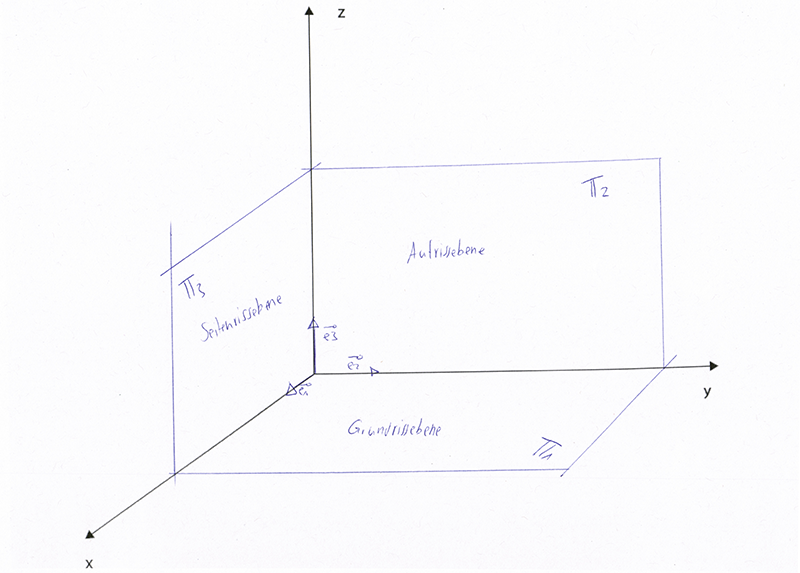
\includegraphics[width=0.8\textwidth]{imgs/rissebene.png}
 \end{center}
je zwei Achsen, eine Ebene bestimmen; Die \underline{Rissebenen} genannt werden, und zwar
\begin{itemize}
	\item
		$\pi_1$ die Grundrissebene (x,y Achse)
	\item 
		$\pi_2$ die Aufrissebene (y,z Achse)
	\item
		$\pi_3$ die Seitenrissebene (x,z Achse)
\end{itemize}
Eine Gerade in $R^3$ schneidet jede Rissebene in einem Punkt, den wir \underline{Spurpunkt nennen}.
Es gibt auch spezielle Lagen, bei denen nur ein oder zwei Spurpunkte entstehen.
\begin{center}
	 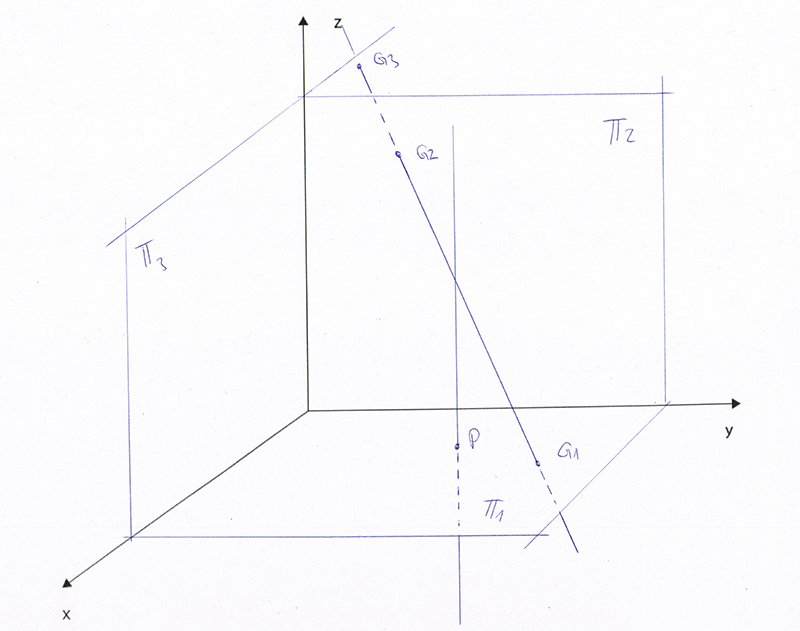
\includegraphics[width=0.8\textwidth]{imgs/spurpunkte.png}
 \end{center}
\begin{itemize}
	\item
		\{$G_1$\} = g $\cap \pi_1$ heisst 1. Spurpunkt
	\item
		\{$G_2$\} = g $\cap \pi_2$ heisst 2. Spurpunkt
	\item
		\{$G_3$\} = g $\cap \pi_3$ heisst 3. Spurpunkt
\end{itemize}
P $\phi_1$ heisst \underline{erstprojizierende Gerade};\\
Sie besitzt nur ein Spurpunkt.\\
Wie können wir nun Punkte, im speziellen Spurpunkt, berechnen?\\
Dazu benötigen wir eine Geradengleichung. Diese suchen wir mit Hile von Vektoren.\\
''Eine Gerad eist durch zwei Punkte A,B bestimmt'' \\
(Ein Axiom der Geometrie)
\begin{center}
	 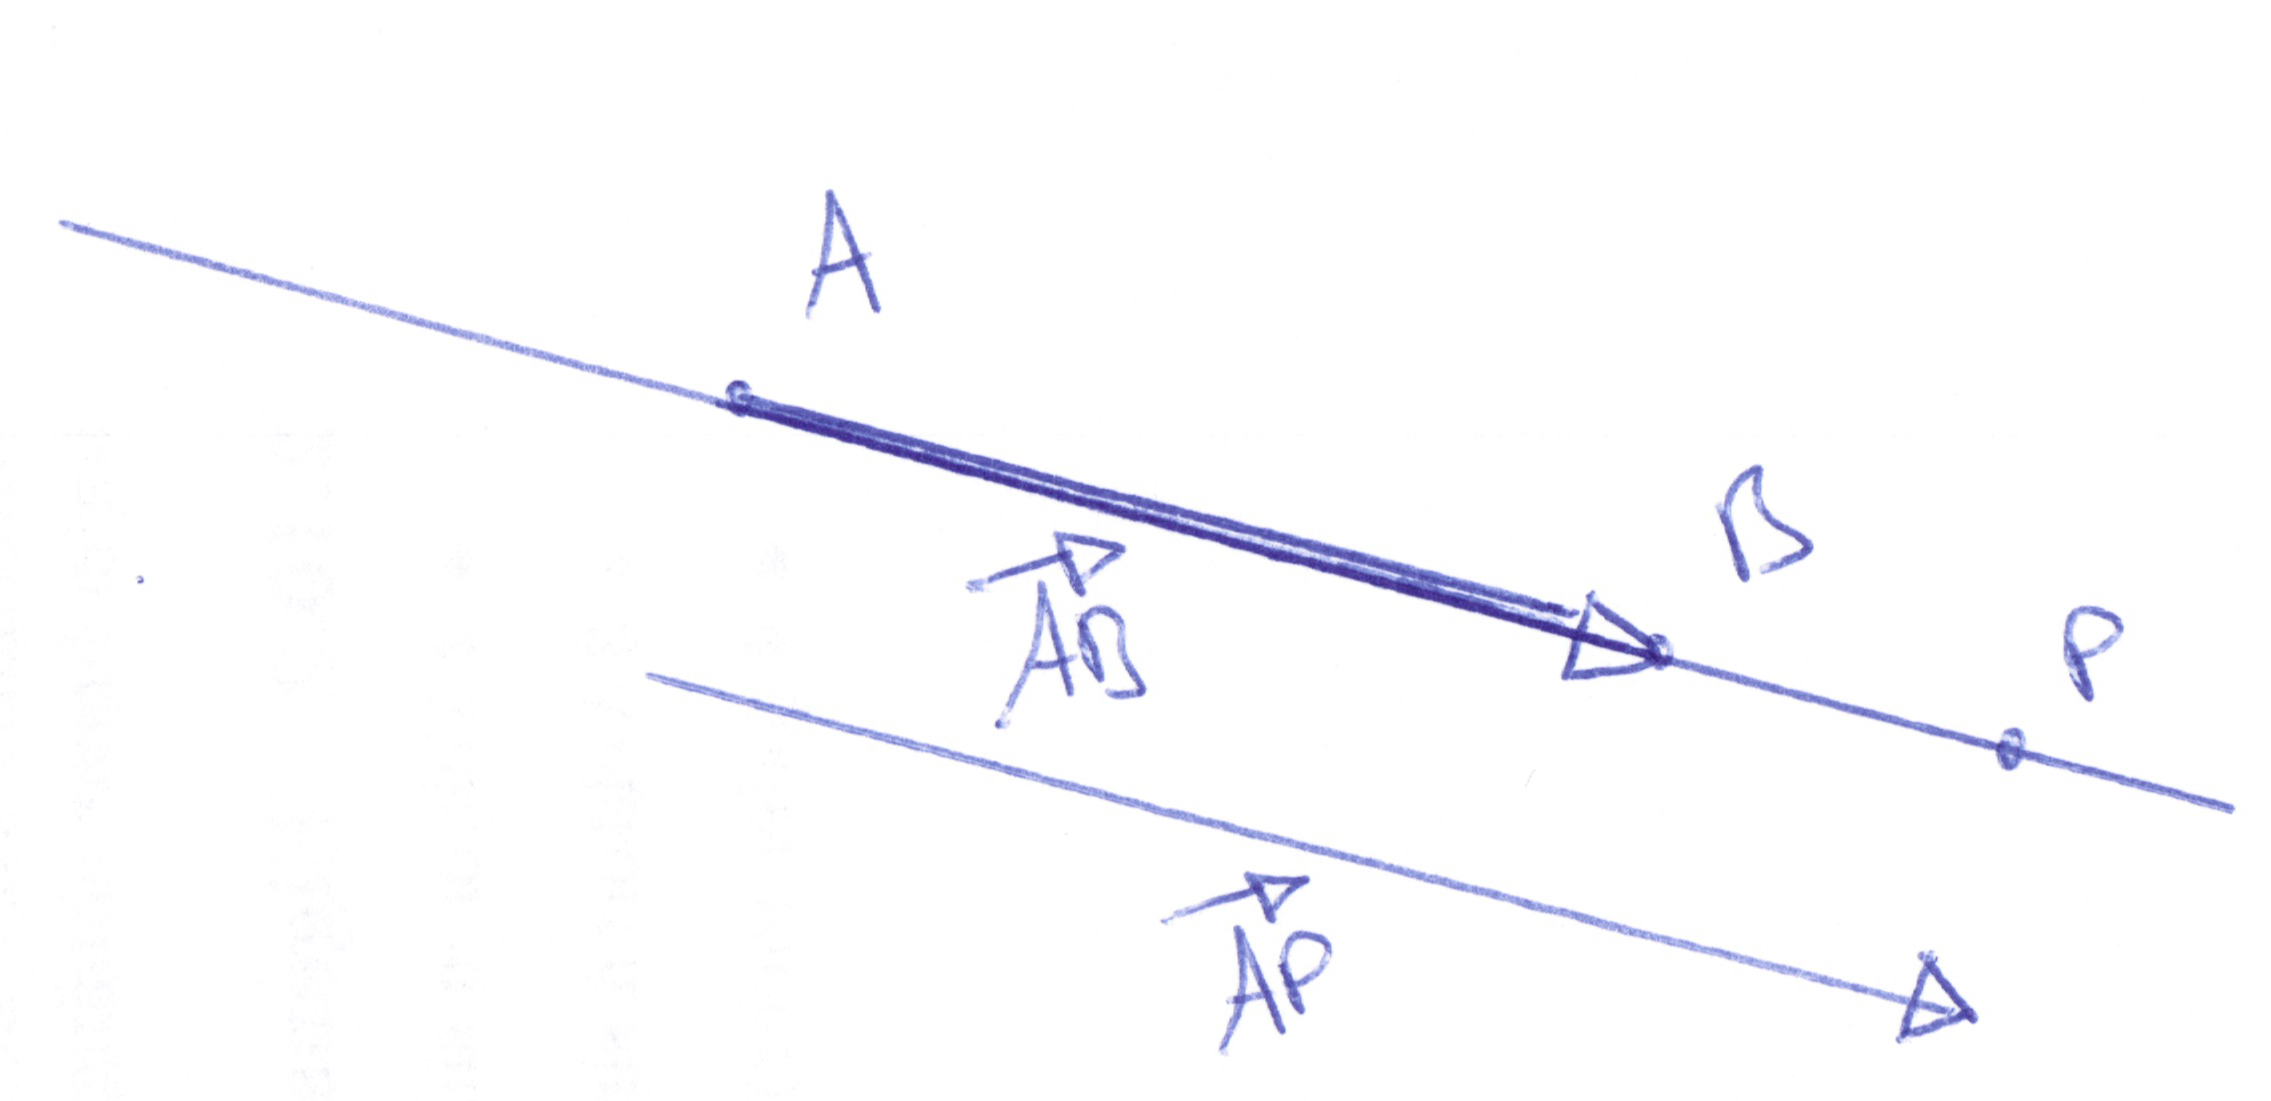
\includegraphics[width=0.8\textwidth]{imgs/geradengleichung.png}
 \end{center}
Damit also $\vec{AB}$ bekannt und für einen beliebigen Punkt  $p$ auf $g$ ist dann $\vec{AP}$
\begin{eqnarray*}
	\vec{AP} = \lambda * \vec{AB}, \lambda \in R\\
	\shortintertext{also}
	\vec{p} - \vec{a} = \lambda(\vec{b} - \vec{a})\\
	\vec{p} = \vec{a} + \lambda(\vec{b} - \vec{a}), \lambda \in R
\end{eqnarray*}
wir haben die Geradengleichung gefunden
\begin{myexample}
	Gerade $g$ durch $A(4/5/-1)$ und $B(2/-3/6)$\\
	Es ist
	\begin{eqnarray*}
		\vec{AB} = \begin{pmatrix}2\\-3\\-6\end{pmatrix}- \begin{pmatrix}4\\5\\-1\end{pmatrix} = \begin{pmatrix}-2\\-8\\7\end{pmatrix}
	\shortintertext{und so}
	g: \vec{p} = \begin{pmatrix}4\\5\\-1\end{pmatrix}+ \lambda\begin{pmatrix}-2\\-8\\7\end{pmatrix}
	\end{eqnarray*}
\end{myexample}
\begin{mydef}
	Wir nennen
	\begin{eqnarray*}
		g: \vec{p} = \vec{a} + \lambda\vec{v}; \lambda \in R
	\end{eqnarray*}
	Die \underline{Parametergleichung} der Geraden g mit dem
	\begin{itemize}
		\item
		\underline{Trägerprunkt} A  (Aufpunkt)
		\item
		\underline{Richtungsvektor} $\vec{v}$
		\item
		\underline{Parameter} $\lambda$
	\end{itemize}
\end{mydef}
\begin{center}
	 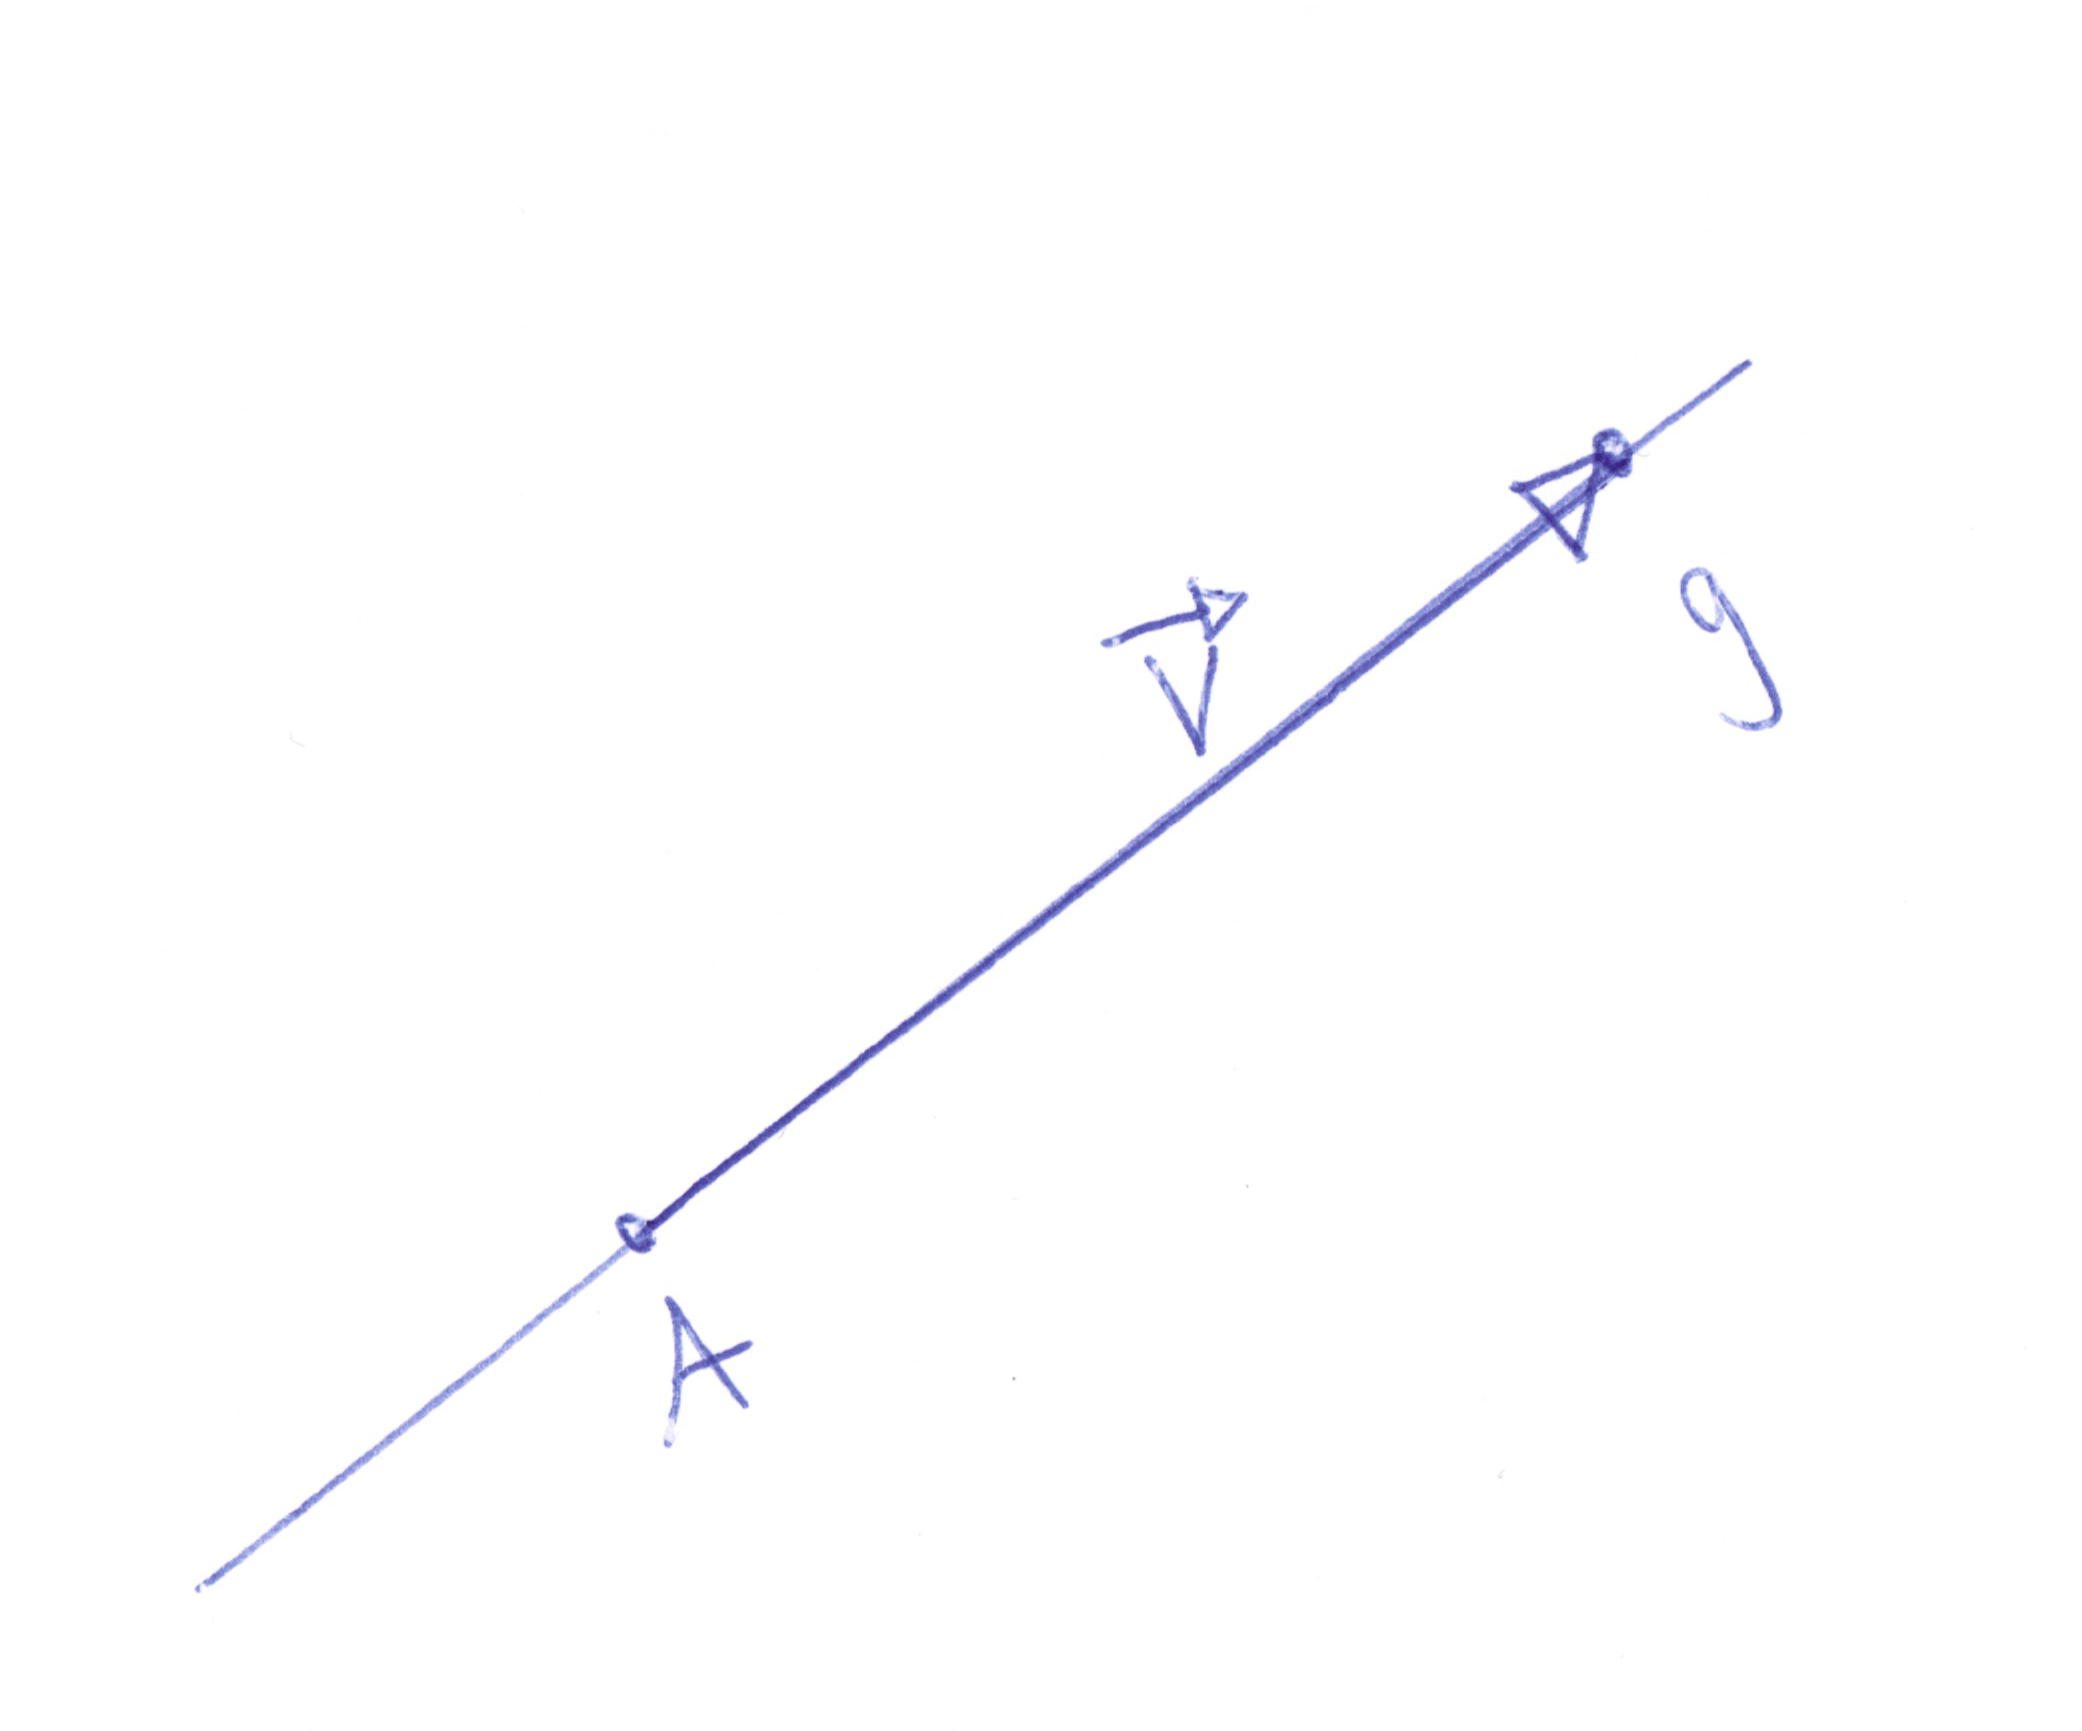
\includegraphics[width=0.8\textwidth]{imgs/parametergleichung.png}
 \end{center}
\begin{myexample}
Welchen zweiten Spurpunkt/$G_2$ besitzt
\begin{equation*}
	g: \vec{p} = \begin{pmatrix}8\\1\\-3\end{pmatrix} + \lambda\begin{pmatrix}2\\-1\\5\end{pmatrix} ?
\end{equation*}
Wir  wissen, $G_2 \in \phi_2$ und somit ist $x = 0$\\
Mit
\begin{eqnarray*}
	\vec{p}\begin{pmatrix}x\\y\\z\end{pmatrix}
	\shortintertext{wird also}
	x &=& 8+2\lambda\\
	y&=& 1-\lambda\\
	z&=& -3 + 5\lambda
\end{eqnarray*} 
Wenn wir die \underline{Geradengleichung komponentenweise} schreiben.\\
Ist
\begin{eqnarray*}
	x&=& 0
	\shortintertext{so wird}
	8+2\lambda &=&0\\
	2\lambda &=& -8\\
	\lambda &=& -4
\end{eqnarray*} 
Damit wird
\begin{eqnarray*}
	y&=& 1-(-4)\\
	y &=& 5\\
	\\
	z &=& -3 + 5(-4)\\
	z&=& -23
	\shortintertext{und so}
	G_2(0/5/-23)
\end{eqnarray*}
\end{myexample}
\begin{myexample}
Welche Parametergleichung hat die erstprojizierende Gerade durch $A(5/-4/7)$?\\
\begin{center}
	 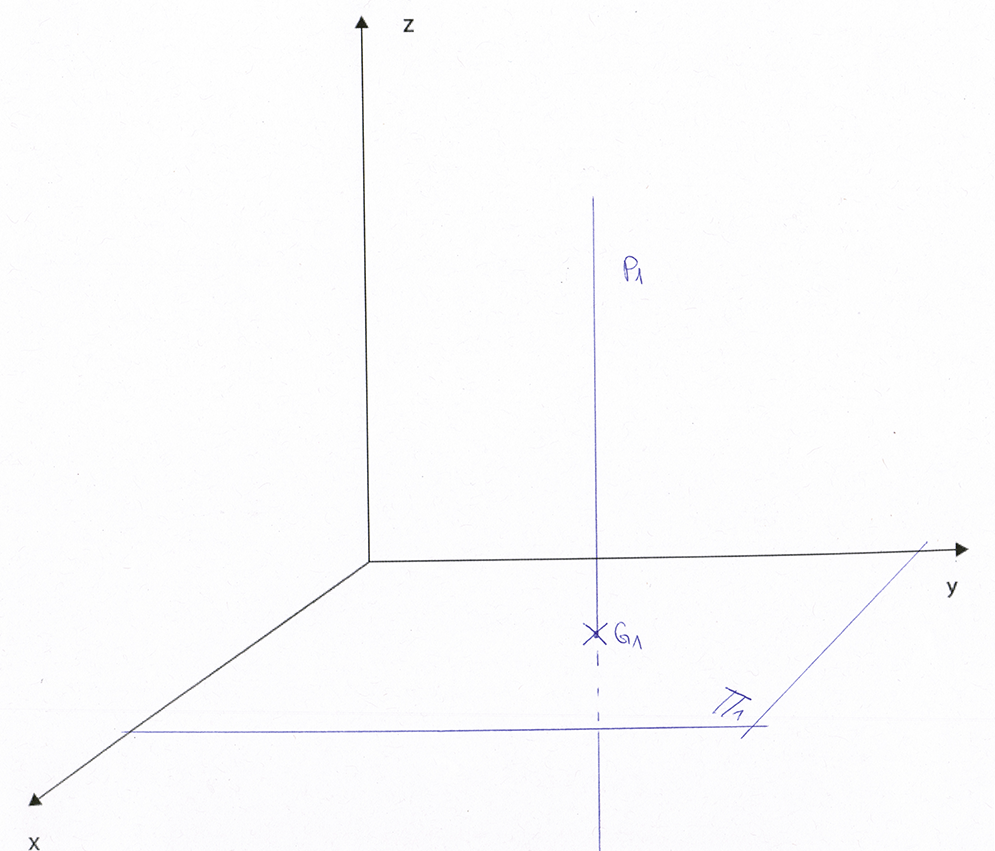
\includegraphics[width=0.8\textwidth]{imgs/erstprojizierende_gerade.png}
 \end{center}
Richtungsvektor ist zum Beispiel
\begin{eqnarray*}
	\vec{e_3} = \begin{pmatrix}0\\0\\1\end{pmatrix}, \vec{v} = \begin{pmatrix}0\\0\\7\end{pmatrix}, \vec{w} = \begin{pmatrix}0\\0\\-3\end{pmatrix}, \text{etc.} 
	\shortintertext{Also}
	p_1: \vec{p} =  \begin{pmatrix}5\\-4\\7\end{pmatrix} + \lambda \begin{pmatrix}0\\0\\1\end{pmatrix} 
\end{eqnarray*}
\end{myexample}
\newpage
\subsection{Hauptgerade}
Eine Gerade, die parallel zu einer Rissebene liegt, heisst \underline{Hauptgerade}\\
Bei einer ersten Hauptgeraden $h_1\parallel \pi_1$ sind also alle z-komponenten gleich.\\
\begin{center}
	 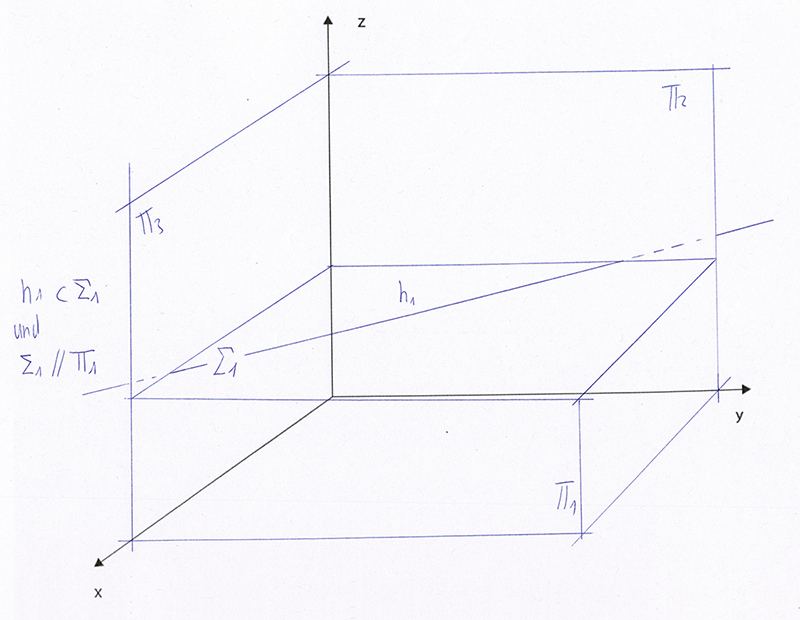
\includegraphics[width=0.8\textwidth]{imgs/hauptgerade.png}
 \end{center}
\begin{myexample}
$h_1$ durch $A(4/-1/5)$ und $B(-2/3/5)$\\
Mit
\begin{eqnarray*}
	\vec{AB} = \begin{pmatrix}-2\\3\\5\end{pmatrix} - \begin{pmatrix}4\\-1\\5\end{pmatrix} = \begin{pmatrix}-6\\4\\0\end{pmatrix}\\
	\shortintertext{wird}
	h_1: \vec{p} = \begin{pmatrix}4\\-1\\5\end{pmatrix} + \lambda\begin{pmatrix}-6\\4\\0\end{pmatrix}	
\end{eqnarray*}
\end{myexample}

\newpage
\subsection{Gegenseitige Lage}
\begin{center}
	 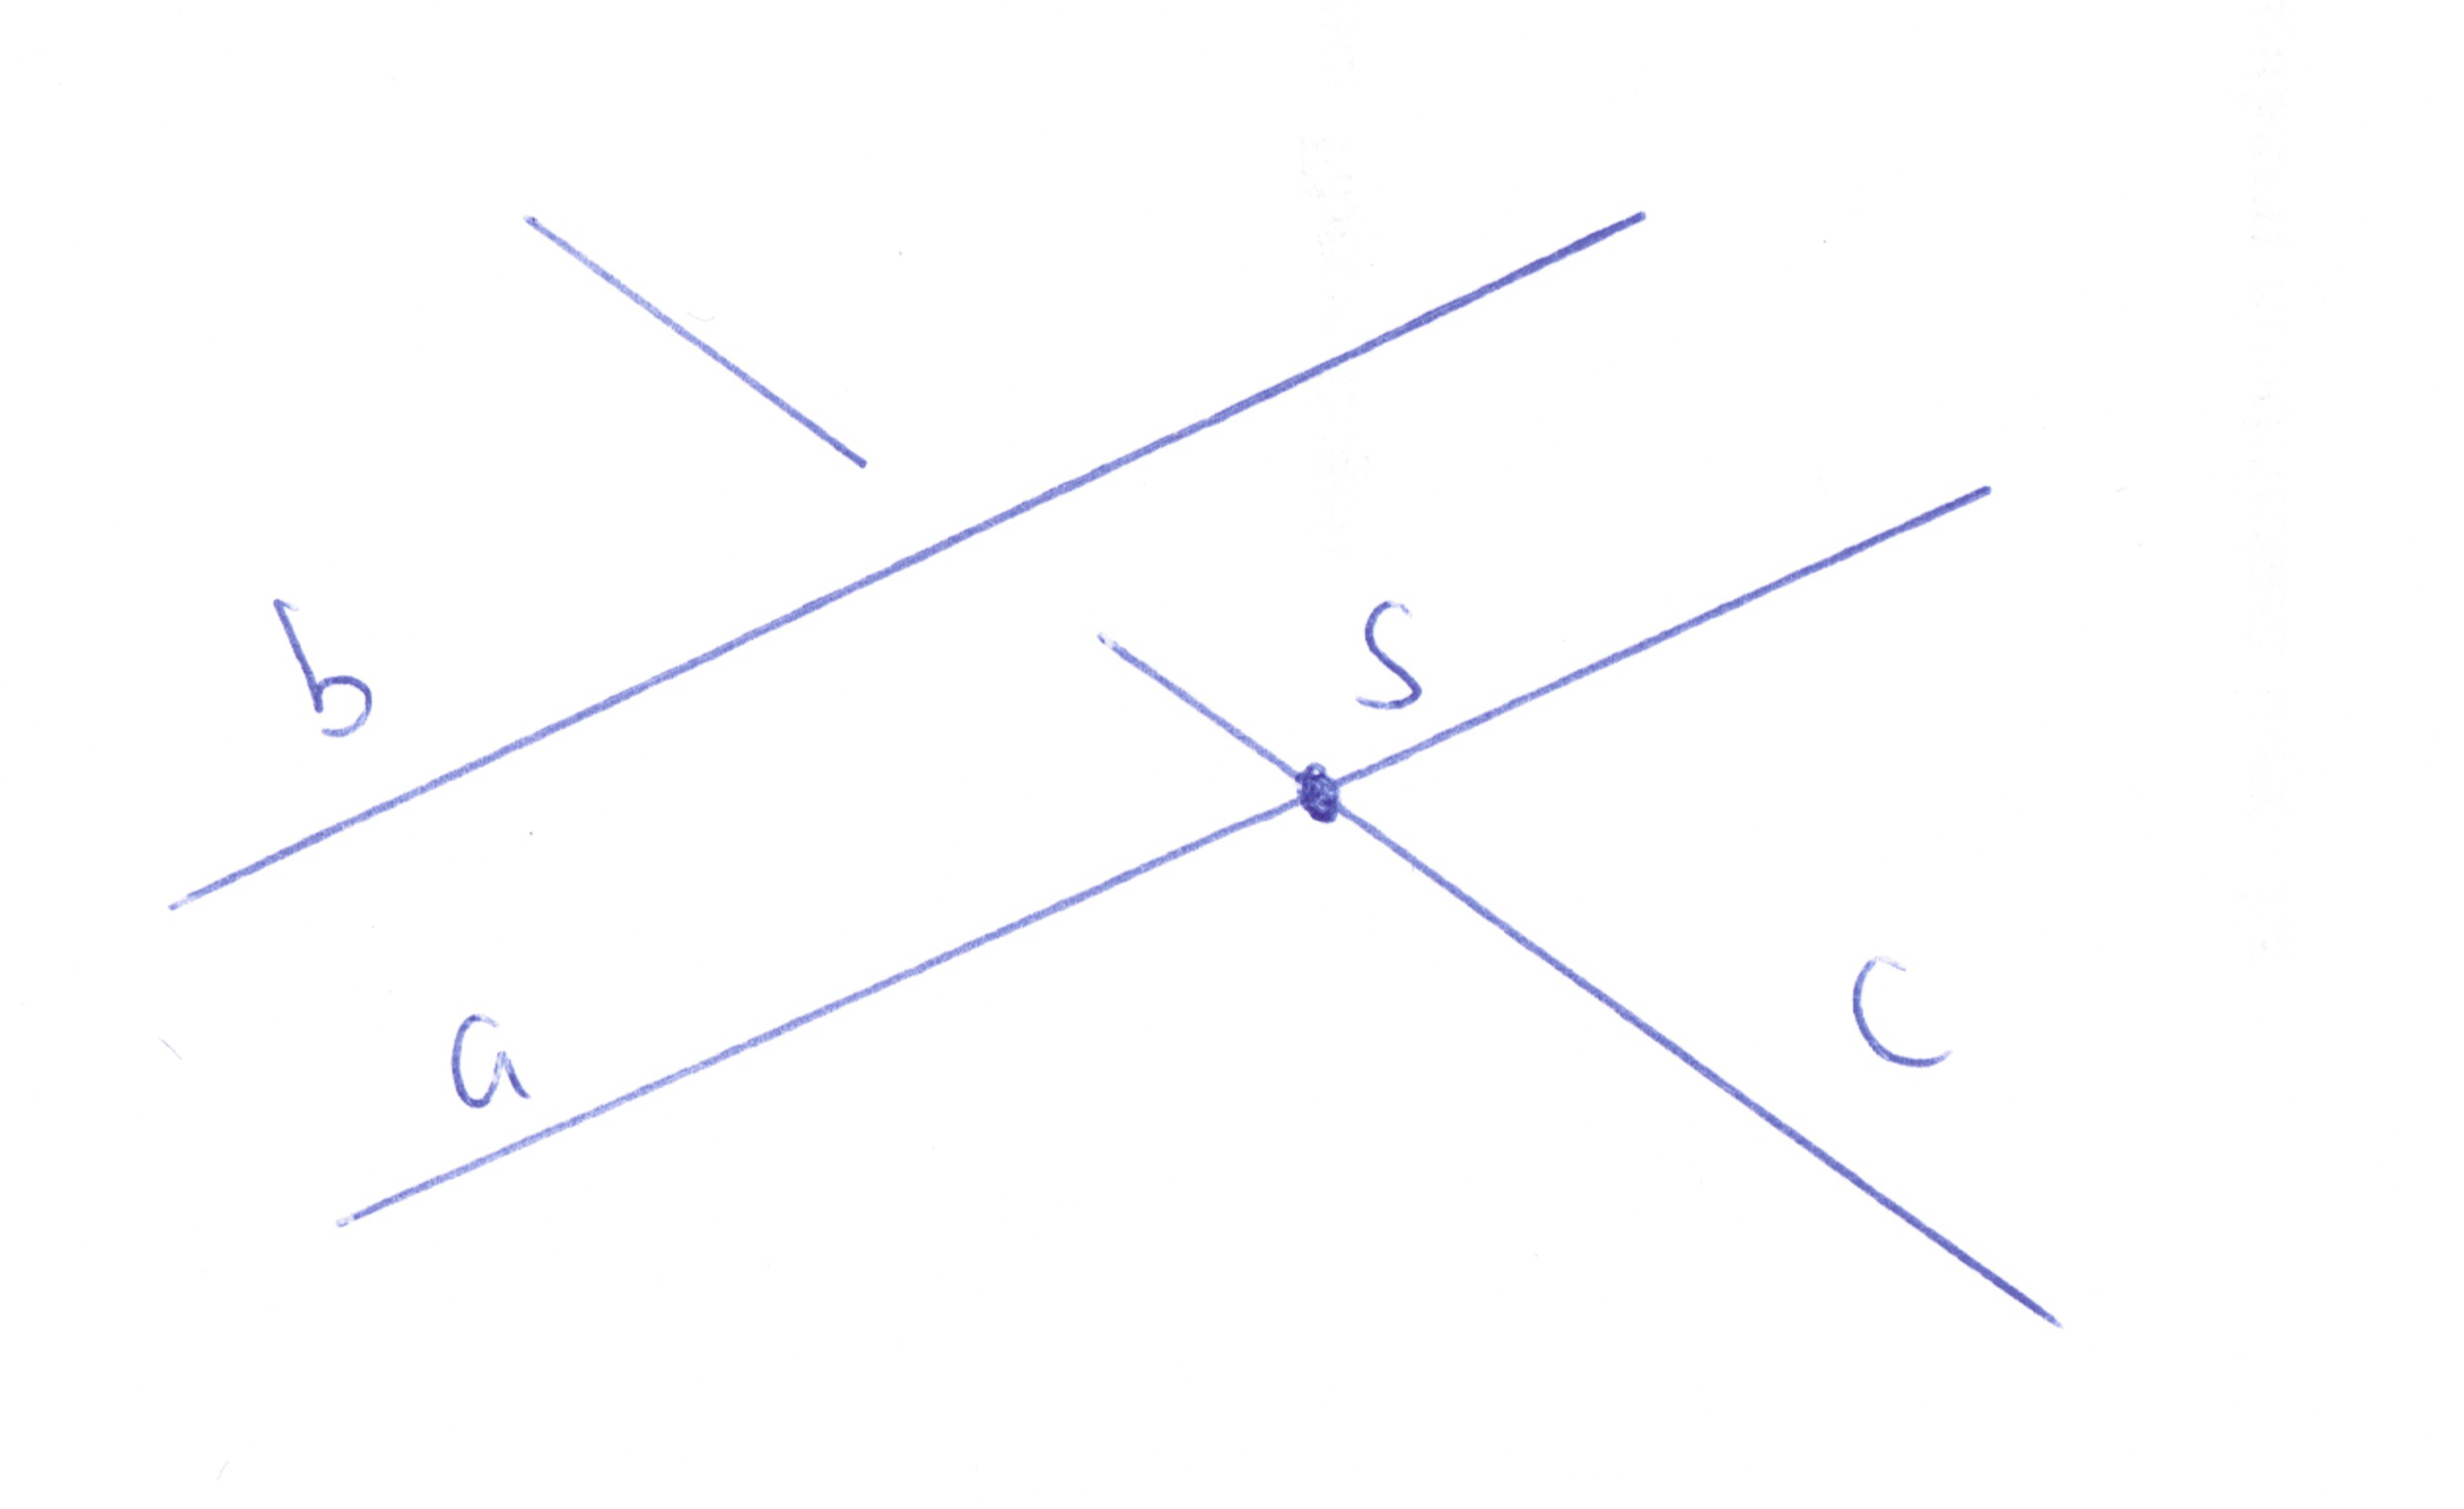
\includegraphics[width=0.8\textwidth]{imgs/gegenseitige_lage.png}
 \end{center}
\begin{itemize}
	\item
	parallel $a \parallel b$\\
	$(a \cap b \not = 0)$
	\item
	schneiden sich: \\
	$a \cap c = \{S\}$
	\item
	windschief:
	$\not (b \parallel c) \land (b \cap c \not = \emptyset)$
\end{itemize}
\newpage
\subsubsection{Parallel}
Kennen wir die beiden Parametergleichungen 
\begin{eqnarray*}
	a: \vec{p} = \vec{a} + \lambda \vec{v}\\
	b: \vec{p} = \vec{b} + \mu\vec{w}\\
\end{eqnarray*}
so finden wir sofort, ob $a \parallel b$ ist,\\
denn dann ist
\begin{center}
$\vec{v}$ und $\vec{w}$ koolinear
\end{center}
\begin{myexample}
	\begin{eqnarray*}
		a: \vec{p} = \begin{pmatrix}1\\3\\-1\end{pmatrix}+ \lambda \begin{pmatrix}12\\15\\6\end{pmatrix}\\
		b: \vec{p} = \begin{pmatrix}-4\\1\\5\end{pmatrix} + \mu \begin{pmatrix}-4\\-5\\2\end{pmatrix}
	\end{eqnarray*}
	$a \parallel b$, denn $\vec{v_a} = (-3)\vec{v_b}$
\end{myexample}
\newpage
\subsubsection{Geschnitten}
Sind die Geraden nicht parallel, wie 
\begin{eqnarray*}
	a: \vec{p} = \begin{pmatrix}2\\1\\2\end{pmatrix}+ \lambda \begin{pmatrix}-1\\3\\4\end{pmatrix}\\
	b: \vec{p} = \begin{pmatrix}1\\2\\-9\end{pmatrix} + \mu \begin{pmatrix}3\\1\\1\end{pmatrix}
\end{eqnarray*}
So suchen wir einen Schnittpunkt.\\
\begin{center}
	 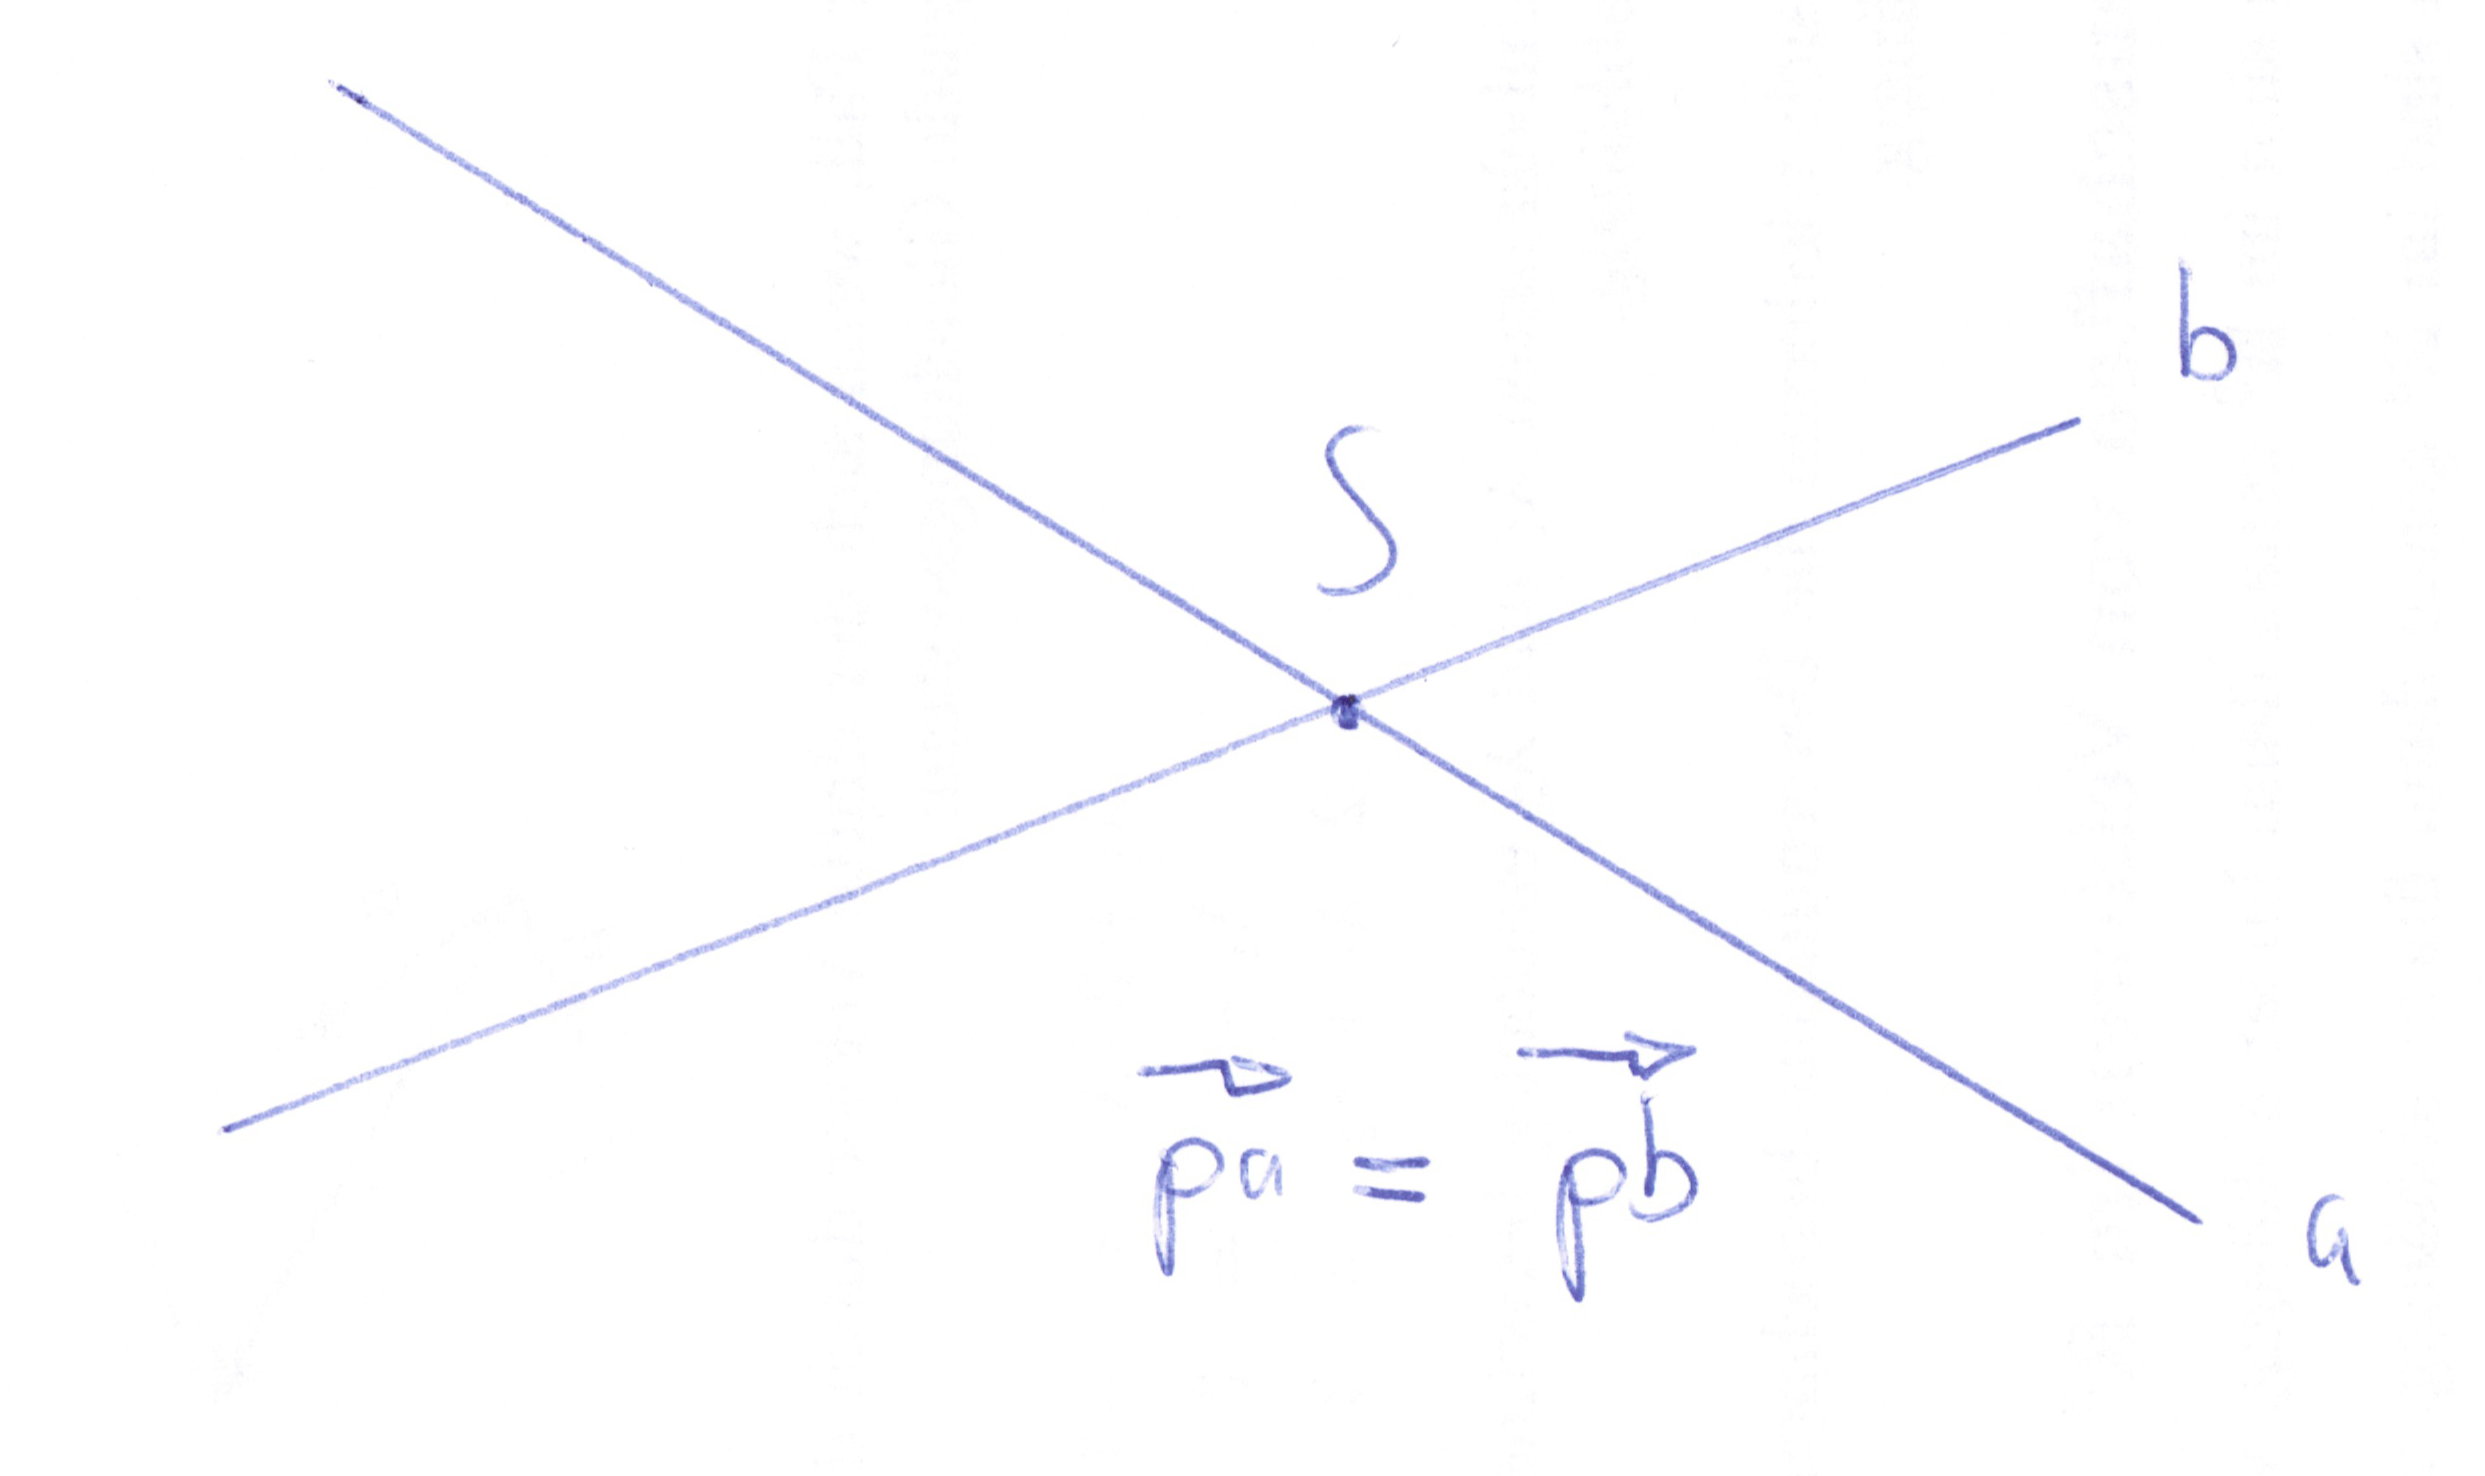
\includegraphics[width=0.8\textwidth]{imgs/schnittpunkt_vektoren.png}
 \end{center}
mit
\begin{equation*}
	\vec{pa} = \vec{pb}
\end{equation*}
also komponentenweise
\begin{center}
	\begin{tabular}{|lll|l}
		$2 - \lambda 	$&=&$ 1 + 3\mu$&(1)\\
		$1 + 3\lambda $&=&$ 2 + \mu$&(2)\\
		$2 + 4 \lambda $&=&$ -1 + \mu$&(3)
	\end{tabular}
\end{center}
und wir erhalten 3 Gleichungen mit 2 Variabeln.
\begin{eqnarray*}
	(3)-(2): 1 + \lambda = -3\\
	\lambda = -4
	\shortintertext{Eingesetzt in}
	(3): 2-16 = -1 + \mu\\
	\mu = -13
	\shortintertext{Kontrolle mit 1}
	\shortintertext{Mit}
 	\lambda = -4\\
 	\mu = -13
	\shortintertext{Wird}
 	2-(-4)\lambda = 1+3(-13)\mu\\
 	2+4 = 1-39\\
 	6 = -38
\end{eqnarray*}
Also ist $a \not \parallel b$ und $a \cap b \not 0$, \\
also sind $a$ und $b$ windschief.
\newpage
\subsubsection{Windschief}
\begin{center}
	 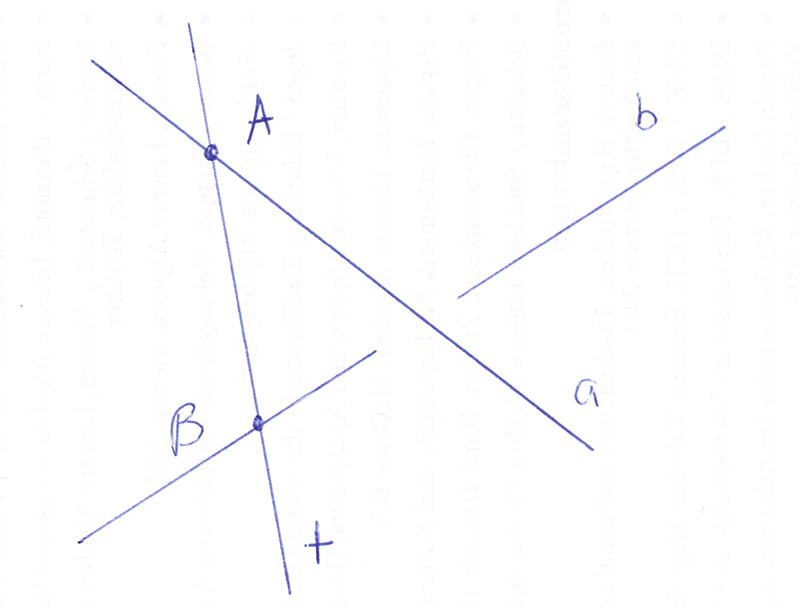
\includegraphics[width=0.8\textwidth]{imgs/transversale.png}
 \end{center}
\begin{mydef}
	Eine Gerade t, die zwei windschiefe Geraden schneidet, heisst \underline{Transversale}
\end{mydef}
\begin{myexample}
	Suche eine Transversale durch $P(2/3/5)$, wobei $P\in a$ mit 
	\begin{eqnarray*}
		a: \vec{p} = \begin{pmatrix}2\\3\\5\end{pmatrix} + \lambda\begin{pmatrix}-1\\1\\8\end{pmatrix}
		\shortintertext{und}
		b:\vec{q} = \begin{pmatrix}-1\\1\\4\end{pmatrix}+\mu\begin{pmatrix}7\\3\\2\end{pmatrix}
	\end{eqnarray*}
	\begin{center}
		 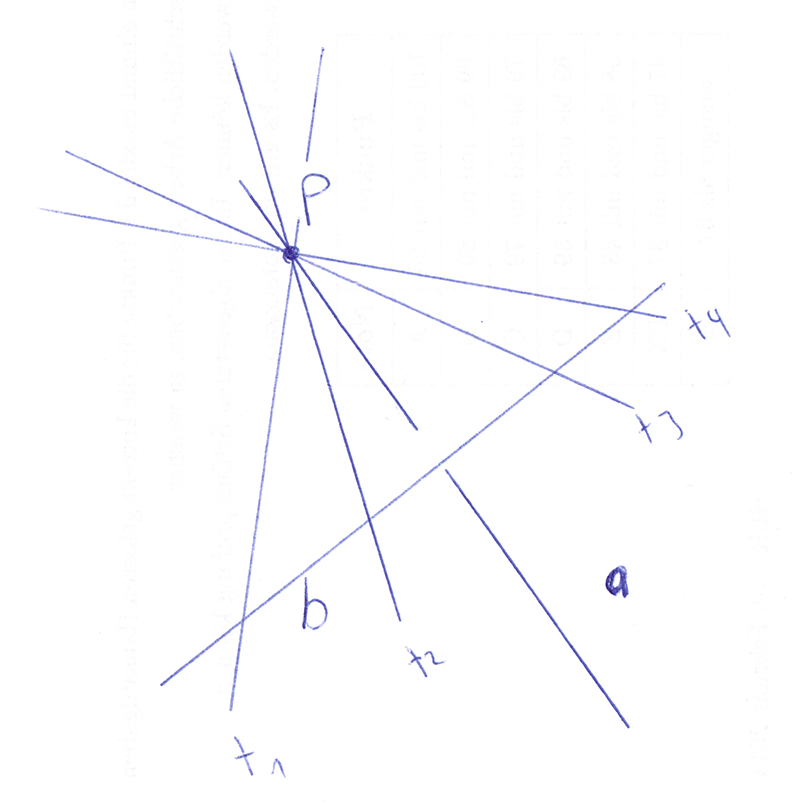
\includegraphics[width=0.8\textwidth]{imgs/transversale_beispiel1.png}
 	\end{center}
	Es gibt unendlich viele. Eine davon finden wir mit der Wahl von $\mu$ in $b: \vec{q}$.  $\mu$ kan beliebig gewählt werden. Durch das Wählen von $\mu$ erhalten wir einen Vektor. Dieser Zeigt auf den Punkt $Q$ auf der Geraden $b$. Der Vektor von $P$ zu $Q$ ist die gesuchte Transversale.
	\begin{eqnarray*}
		\mu = 5\\
		\vec{q}\begin{pmatrix}-1\\1\\4\end{pmatrix} +\begin{pmatrix}35\\15\\10\end{pmatrix} = \begin{pmatrix}34\\16\\14\end{pmatrix}
		\shortintertext{und so}
		\vec{PQ} = \begin{pmatrix}34\\16\\14\end{pmatrix}-\begin{pmatrix}2\\3\\5\end{pmatrix} = \begin{pmatrix}32\\13\\9\end{pmatrix}
		\shortintertext{womit}
		t: \vec{a} = \begin{pmatrix}2\\3\\5\end{pmatrix} + \sigma\begin{pmatrix}32\\13\\9\end{pmatrix}
	\end{eqnarray*}
\end{myexample}
\begin{myexample}
	Suche eine Transversale, die sowohl zu
	\begin{eqnarray*}
		a: \vec{q} = \begin{pmatrix}2\\3\\5\end{pmatrix} + \lambda \begin{pmatrix}0\\2\\1\end{pmatrix} 
		\shortintertext{als auch}
		b: \vec{p} = \begin{pmatrix}1\\6\\-2\end{pmatrix} + \mu \begin{pmatrix}3\\-2\\0\end{pmatrix} 
	\end{eqnarray*}
	senkrecht steht.\\
	\begin{center}
		 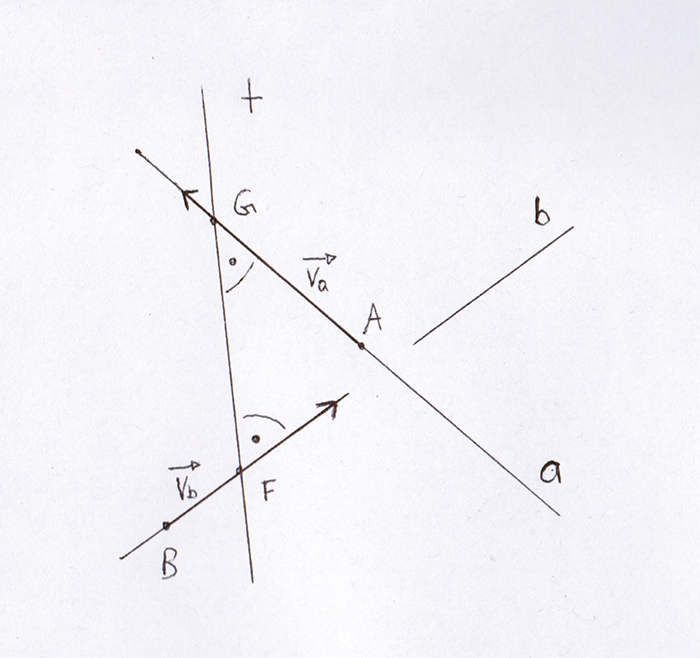
\includegraphics[width=0.8\textwidth]{imgs/transversale_beispiel2.png}
 	\end{center}
	Es gibt genau eine solche Transversale.\\
	Sind F und G die Schnittpunkte, so ist
	\begin{eqnarray*}
		\vec{FG} * \vec{V_b} = 0 \land \vec{FG} * \vec{V_a} = 0
		\shortintertext{Mit $F \in b$ wird}
		F(1+3\mu/6-2\mu/-2)
		\shortintertext{und $G \in a$, also}
		G(2/3+2\lambda/5+\lambda)
		\shortintertext{so wird}
		\vec{FG} \begin{pmatrix}2 -(1+3\mu)\\3+2\lambda-(6-2\mu)\\5+\lambda-(-2)\end{pmatrix} \\
		=\begin{pmatrix}1-3\mu)\\-3+2\lambda+2\mu)\\7+\lambda\end{pmatrix}
	\end{eqnarray*}
	und damit
	\begin{eqnarray*}	
		\vec{FG}* \vec{V_a} &=& (1-3\mu) *0+(-3+2\lambda+2\mu)*2+(7+\lambda)*1\\
		&=&-6+4\lambda+4\mu+7+\lambda\\
		&=&5\lambda+4\mu+1\\
		\\
		\vec{FG}* \vec{V_b} &=& (1-3\mu)*3+(-3+2\lambda+2\mu)(-2)\\
		&=& 3-9\mu + 6-4\lambda -4\mu\\
		&=& -4\lambda -13\mu+9\\
	\end{eqnarray*}
	womit wir
	\begin{eqnarray*}	
		\begin{vmatrix}5\lambda+4\mu+1&=&0\\-4\lambda-13\mu+9 &=& 0\end{vmatrix}
	\end{eqnarray*}
	erhalten. Weiter ist dann
	\begin{eqnarray*}	
		-49\mu + 49 &=&0\\
		\mu &=& 1
		\shortintertext{und so}
		5\lambda + 4 +1&=& 0\\
		\lambda &=& -1
	\end{eqnarray*}	
	Damit wird
	\begin{eqnarray*}	
		F(4/4/-2),G(2/1/4)
		\shortintertext{und}
		\vec{FG} = \begin{pmatrix}2-4\\1-4\\4-(-2)\end{pmatrix} = \begin{pmatrix}-2\\-3\\6\end{pmatrix}
		\shortintertext{also}
		t:\vec{p} \begin{pmatrix}4\\4\\-2\end{pmatrix} + \alpha \begin{pmatrix}-2\\-3\\6\end{pmatrix} 
	\end{eqnarray*}	
	Ausserdem haben wir nun noch den \underline{Abstand der Windschiefen Geraden}
	\begin{equation*}
		|\vec{FG}| = \sqrt{(2)^2+(-3)^2+6^2} = 7
	\end{equation*}
	mit dem \underline{Fusspunkt} F und G eralten.
\end{myexample}
\newpage
\section{Ebenen}
\begin{center}
	 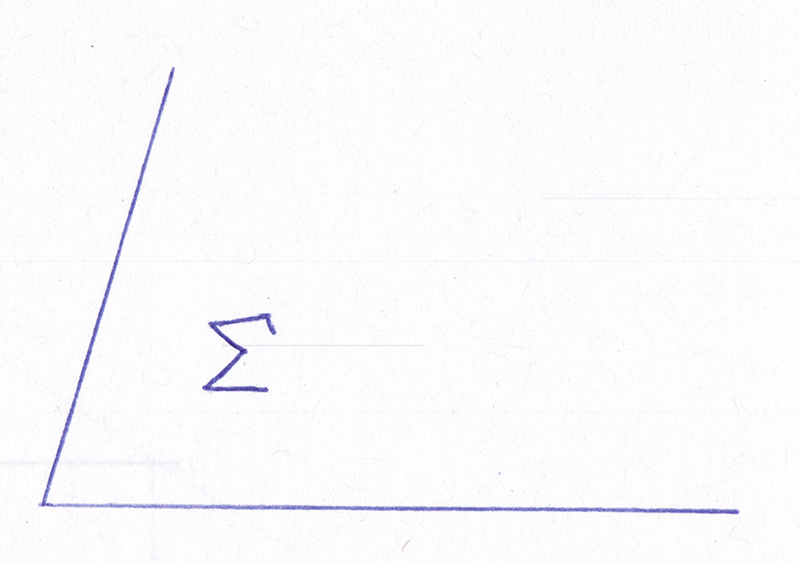
\includegraphics[width=0.8\textwidth]{imgs/ebenen.png}
 \end{center}
Eine Ebene ist bestimmt durch 
\begin{itemize}
	\item
	3 Punkte, die nicht auf derselben Geraden liegen
	\item
	2 paralelle Geraden
	\item
	zwei sich schneidende Geraden
	\item
	Eine Gerade g und ein Punkt $p \not \in g$
\end{itemize}
Ebenen bezeichnen wir mit griechischen Grossbuchstaben
\begin{equation*}
	\Delta,\Omega,\Sigma,\Pi, \ldots
\end{equation*}
Kennen wir 3 nicht auf derselben Geraden liegende Punkte $A,B,C \in \Sigma$,
\begin{center}
	 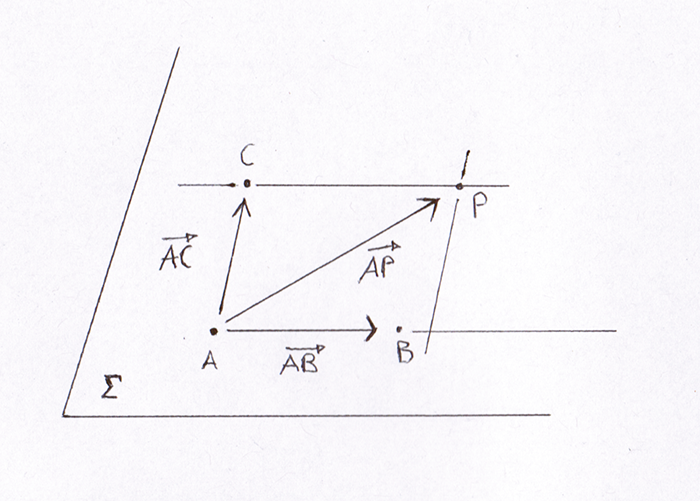
\includegraphics[width=0.8\textwidth]{imgs/ebenen_beispiel1.png}
 \end{center}
und suchen einen weiteren Punkt $P \in \Sigma$,
\begin{eqnarray*}
	\vec{AP} &=& \lambda\vec{AB}+\mu\vec{AC}; \lambda, \mu \in R\\
	\Sigma: \vec{p} &=& \vec{a}+\lambda\vec{AB}+\mu\vec{AC}
\end{eqnarray*}
\begin{myexample}
	$\Omega$ durch A(3/1/-4), B(-2/1/5) und C(3/4/4)
	Mit
	\begin{eqnarray*}
		\vec{AB}= \begin{pmatrix}-5\\0\\9\end{pmatrix}, \vec{AC} = \begin{pmatrix}0\\3\\8\end{pmatrix}\\
		\shortintertext{wird} \Omega: \vec{p}=\begin{pmatrix}3\\1\\-4\end{pmatrix}+\lambda\begin{pmatrix}-5\\0\\9\end{pmatrix}+\mu\begin{pmatrix}0\\3\\8\end{pmatrix}
	\end{eqnarray*}
\end{myexample}
 \begin{center}
	 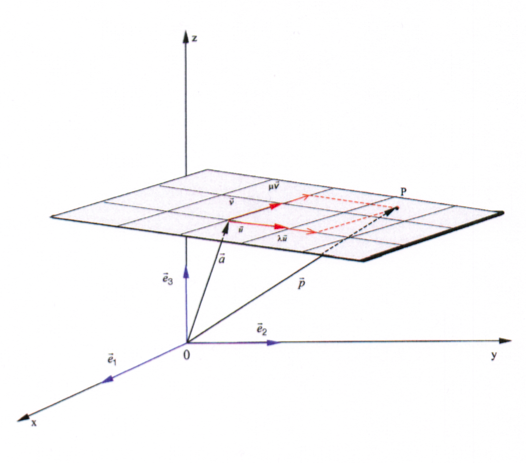
\includegraphics[width=0.8\textwidth]{imgs/parametergleichung_ebene.png}
 \end{center}
\begin{mydef}
	Wir nennen
	\begin{equation*}
		\Sigma: \vec{p} = \vec{a} + \lambda\vec{u}+\mu\vec{v}, \lambda, \mu \in R
	\end{equation*}
	Die Parametergleichung der Ebene mit
	\begin{itemize}
		\item
			den Richtungsvektor $\vec{u}$,$\vec{v}$
		\item
			dem Trägerpunkt A
		\item
			den Parameter $\lambda$,$\mu$
	\end{itemize}
	Vektoriell ist eine Eben also durch 2 lin. unabhängige Vektoren und ein Punkt bestimmt.
\end{mydef}
\newpage
Schreiben wir die Parametergleichung 
\begin{eqnarray*}
	\Lambda: \vec{p} = \begin{pmatrix}2\\-3\\5\end{pmatrix} + \lambda\begin{pmatrix}4\\-1\\3\end{pmatrix}+\mu\begin{pmatrix}1\\-2\\-1\end{pmatrix}  
	\shortintertext{komponentenweise}
	\begin{tabular}{|l|l}
		x = 2+4 $\lambda$ +$\mu$&(1)\\
		y = -3 - $\lambda$ -2 $\mu$&(2)\\
		z = 5 + 3$\lambda$- $\mu$&(3)
	\end{tabular}
\end{eqnarray*}
So können wir mit 2 der 3 Gleichungen $\lambda$ und $\mu$ berechnen und dann diese Resultate in die 3. Gleichung einsetzen.\\
Rechnen wollen wir aber mit dem Gaus-Algorithmus
\begin{eqnarray*}
	(1)+(3): x+z = 7+ 7\lambda\\
	2(1)+(2): 2x+y = 1+7\lambda\\
	x+z -2x -y = 6\\
	\Lambda: -x-y+z-6= 0\\
	\Lambda: x+y -z + 6 = 0
\end{eqnarray*}
\begin{mydef}
	Wir nennen 
	\begin{equation*}\Sigma: ax+by+cz+d=0\end{equation*}
	(a,b,c und d nicht gleichzeitig 0)
\end{mydef}
die \underline{Koordinatengleichung von $\Sigma$}
\begin{myexample}
	Welche Koordinatengleichung hat die Grundrissebene?
	\begin{equation*}
		\Pi_1: z = 0
	\end{equation*}
	Die Koordinatengleichung definiert was ein Punkt erfüllen muss um in dieser Ebene zu liegen.
\end{myexample}
\begin{mydef}
Eine Ebene $\Sigma$, die parallel zu einer Rissebene liegt, \underline{Hauptebene}
\end{mydef}
\begin{center}
	 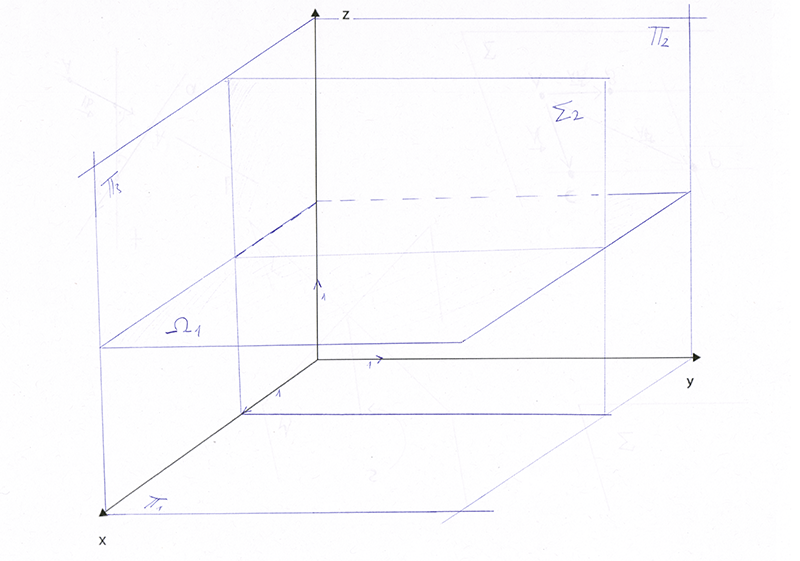
\includegraphics[width=0.8\textwidth]{imgs/hauptebenen.png}
 \end{center}
$\Omega \parallel \Pi_1$ ist eine \underline{erste} und \\
$\Sigma \parallel \Pi_2$ ist eine \underline{zweite} Hauptebene.\\
Der Index bestimmt zu welcher Ebene die Hauptebene parallel ist.
\begin{myexample}
	Welche Koordinatengleichung und welche Parallelgleichung hat die zweite Hauptebene $\Sigma_2$, die Punkt $A(4/5/3)$ enthält.\\
	Koordinatengleichung:\\
	\begin{eqnarray*}
		\Sigma_2: x= 4\\
		\Sigma_2: x-4 = 0
		\shortintertext{Parametergleichung: Richtungsvektoren sind $\vec{e_2}$ und $\vec{e_3}$, also}
		\Sigma_3: \vec{p}= \begin{pmatrix}4\\5\\3\end{pmatrix} + \lambda \begin{pmatrix}0\\1\\0\end{pmatrix} + \mu\begin{pmatrix}0\\0\\1\end{pmatrix} 
	\end{eqnarray*}
\end{myexample}
\begin{mydef}
Eine Ebene, die Senkrecht zu einer Rissebene steht, heisst \underline{projizierende} Ebene.
\end{mydef}
\begin{center}
	 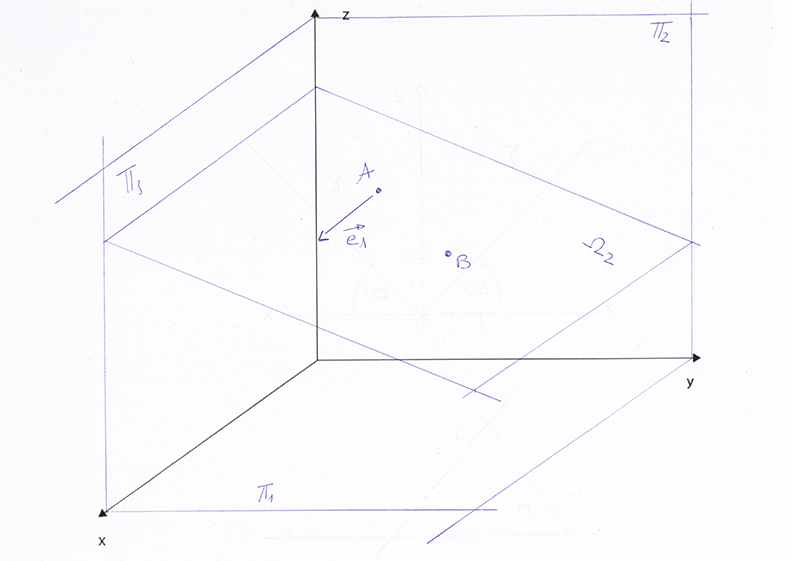
\includegraphics[width=0.8\textwidth]{imgs/zweitprojizierende_ebene.png}
 \end{center}
$\Omega_2 \perp \Pi_2$ ist eine \underline{zweitprojizirende} Ebene. \\
Ist $A(1/2/6), B(4/4/1)$ so ist $\vec{AB}$ der eine und $\vec{e_1}$ der andere Richtungsvektor.\\
Also wird 
\begin{eqnarray*}
	\Omega_2: \vec{p} = \begin{pmatrix}1\\2\\6\end{pmatrix}+\lambda\begin{pmatrix}3\\2\\6-5\end{pmatrix}+\mu \begin{pmatrix}1\\0\\0\end{pmatrix}
	\shortintertext{und so}
	\begin{tabular}{|l|l}
		x = 1 + 3$\lambda$ + $\mu$& (1)\\
		y= 2+2$\lambda$& (2)\\
		z = 6-5$\lambda$& (3)
	\end{tabular}
	5(2) + 2(3): 5y + 2z = 22\\
	\Omega_2: 5y+2z-22=0
\end{eqnarray*}
Also liegen $(4/4/1), (7/4/1),(-9/4/1) \ldots in \Omega_2$,  denn x ist \underline{frei wählbar}.\\
Eine Variable frei wählbar $\to$ eine projizierende Ebene\\
\begin{center}
	 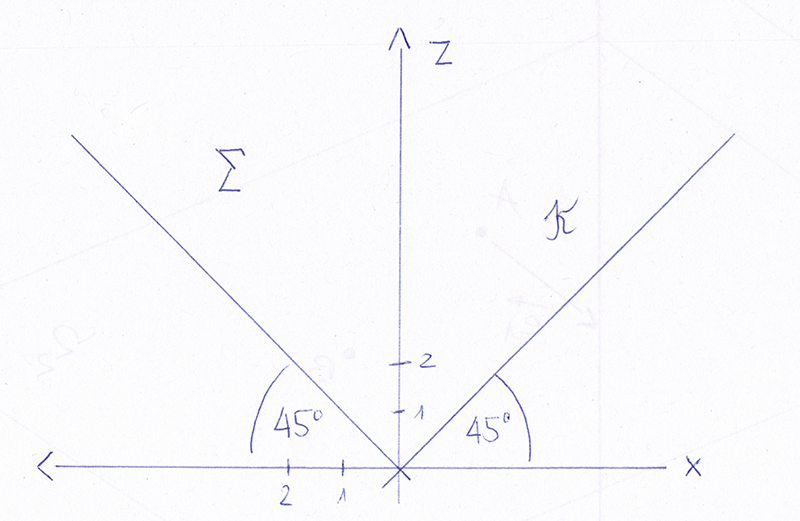
\includegraphics[width=0.8\textwidth]{imgs/symmetrie_koinzidenzebene.png}
 \end{center}
$\Sigma$ heisst \underline{symmetrieebene} und $\kappa$ heisst die \underline{Koinzidenzebene}\\
Es ist
\begin{eqnarray*}
	\Sigma: x = z\\
	\Sigma: x-z =0\\
	\shortintertext{und}
	\kappa: x = -z\\
	\kappa: x + z = 0
\end{eqnarray*} 
\newpage
\subsection{Schnittprobleme}
\subsubsection{Schnitt Gerade mit Ebene}
\begin{center}
	 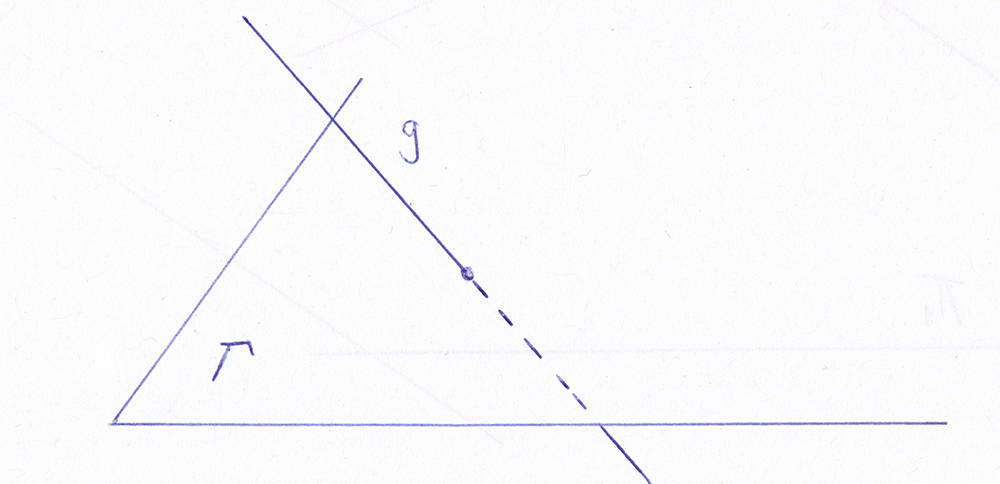
\includegraphics[width=0.8\textwidth]{imgs/durchstosspunkt.png}
 \end{center}
$\{D\} = g \cap \Gamma$ heisst \underline{Durchstosspunkt}\\
\\
Ist 
\begin{eqnarray*}
	\Gamma: \vec{p} = \begin{pmatrix}-1\\3\\9\end{pmatrix} + \lambda\begin{pmatrix}1\\-1\\4\end{pmatrix} + \mu\begin{pmatrix}1\\2\\-2\end{pmatrix}
	\shortintertext{und}
	g: \vec{p} = \begin{pmatrix}7\\6\\3\end{pmatrix}+ \alpha \begin{pmatrix}2\\-1\\-2\end{pmatrix}
	\shortintertext{so muss $\vec{p_\gamma} = \vec{p_g}$ sein, also komponentenweise}
	\begin{tabular}{|l|l}
		$-1+\lambda+\mu = 7+ 2\alpha$& (1)\\
		$3-\lambda + 2 \mu = 6- \alpha$& (2)\\
		$9+ 4 \lambda -2\mu = 3 -2\alpha$& (3)
	\end{tabular}
	\shortintertext{und wir berechnen $\alpha$}
	(1)+(2): 2+ 3\mu = 13 + \alpha\\
	4(2)+(3): 21 + 6\mu = 27-6\alpha\\
	-17 = -1 + 8\alpha\\
	-16 = 8\alpha
	\alpha = -2
\end{eqnarray*}
Setzen wir $\alpha$ein, erhalten wir den Punkt\\
\begin{equation*}D(3/8/7)\end{equation*}
\begin{myexample}
	Ist
	\begin{eqnarray*}
		\Omega: 2x-y+3z + 1= 0
		\shortintertext{und}
		g: \vec{p} = \begin{pmatrix}3\\-4\\-1\end{pmatrix}+ \lambda \begin{pmatrix}2\\-1\\1\end{pmatrix}
		\shortintertext{so ist}
		x = 3+ 2\lambda\\
		y = -4 - \lambda\\
		z = -1 + \lambda
		\shortintertext{was eingesetzt in $\Omega$ zu}
		2(3+2\lambda) - (-4-\lambda)+ 3(-1 + \lambda) + 1 = 0\\
		6+ 4\lambda + 4 + \lambda + -3 + 3 \lambda + 1 = 0\\
		8\lambda = -8\\
		\lambda = -1
		\shortintertext{führt}
		\shortintertext{somit wird}
		D(1/-3/-2)
	\end{eqnarray*}
\end{myexample}
\newpage
\subsubsection{Schnitt Ebene mit Ebene}
\begin{center}
	 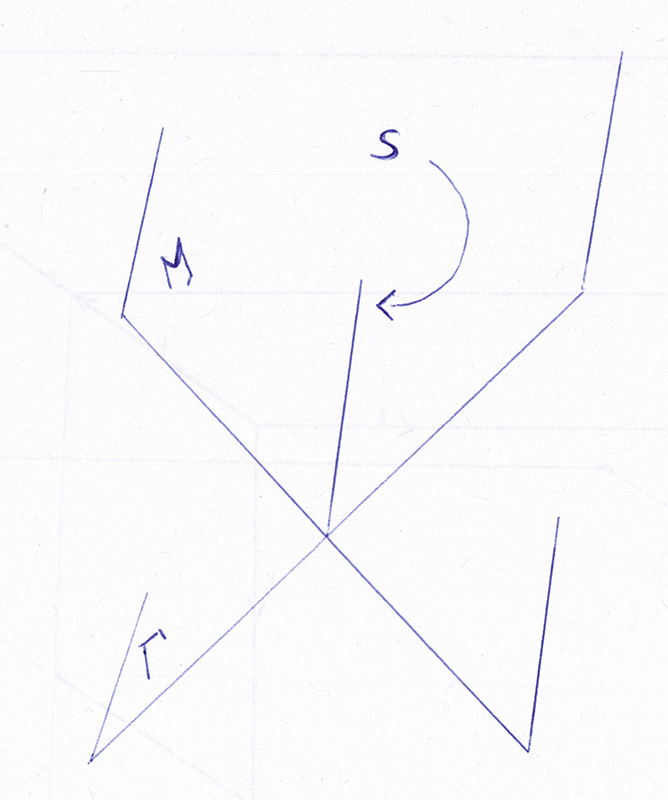
\includegraphics[width=0.8\textwidth]{imgs/schnittgerade.png}
 \end{center}
$\{S\} = \Gamma \cap \Sigma $ heisst \underline{Schnittgerade}\\
Ist
\begin{eqnarray*}
	\Gamma: x-2y + 2z -1 = 0
	\shortintertext{und}
	\Sigma: 2x -3y -z + 2 = 0
	\shortintertext{so wird}
	\begin{tabular}{|l|l}
		x-2y+2z-1= 0&(1)\\
		2x-3y-z+2 = 0&(2)
	\end{tabular}
\end{eqnarray*}
Und wir können eine Variable frei wählen.\\
Zum Beispiel
\begin{equation*}
	x = 0, y = 1, z = 3 \ldots
\end{equation*}
Da wir aber einen Parameter benötigen, wählen wir
\begin{eqnarray*}
	x = \lambda
	\shortintertext{Damit erhalten wir}
	\begin{tabular}{|l|l}
		$\lambda-2y+2z-1 = 0$& (1)\\
		$2\lambda -3y -z + 2 = 0$&(2)
	\end{tabular}\\
	\\
	(1)+(2): 5\lambda -8y + 3 = 0\\
	8y = 3 + 5\lambda\\
	y = \frac{3}{8} + \frac{5}{8} \lambda\\
	3(1) - 2(2): -\lambda + 8z -7 = 0\\
	8z = 7+ \lambda\\
	z = \frac{7}{8} + \frac{1}{8}\lambda\\
	\shortintertext{zusammengefasst}
	x = \lambda\\
	y = \frac{3}{8} + \frac{5}{8}\lambda\\
	z = \frac{7}{8} + \frac{1}{8}\lambda\\
	S : \vec{p} = \begin{pmatrix}0\\\frac{3}{8}\\\frac{7}{8}\end{pmatrix}+\lambda\begin{pmatrix}1\\\frac{5}{8}\\\frac{1}{8}\end{pmatrix}
\end{eqnarray*}
Die Länge von $\vec{v}$ ist beliebeig\\
also
\begin{equation*}
	S: \vec{p} = \begin{pmatrix}0\\\frac{3}{8}\\\frac{7}{8}\end{pmatrix}+\lambda\begin{pmatrix}8\\5\\1\end{pmatrix}
\end{equation*}
Einen ganzzahligen Trägerpunkt erhalten wir mit der Wahl von
\begin{eqnarray*}
	\lambda &=& \frac{1}{8}
	\shortintertext{dann wird}
	x&=& 0 + \frac{1}{8} * 8 = 1\\
	y&=& \frac{3}{8} + \frac{1}{8} * 5 = 1\\
	z&=& \frac{7}{8} + \frac{1}{8} * 1 = 1
	\shortintertext{also}
	S: \vec{p} &=& \begin{pmatrix}1\\1\\1\end{pmatrix}+\lambda\begin{pmatrix}8\\5\\1\end{pmatrix}
\end{eqnarray*}
\newpage
Kennen wir die Parametergleichung
\begin{eqnarray*}
	\Sigma: \vec{p} = \begin{pmatrix}2\\0\\-1\end{pmatrix}+\lambda\begin{pmatrix}1\\2\\-3\end{pmatrix} + \mu \begin{pmatrix}-1\\1\\3\end{pmatrix}
	\shortintertext{und}
	\Phi: \vec{p} = \begin{pmatrix}4\\-1\\1\end{pmatrix}+\sigma\begin{pmatrix}-2\\1\\2\end{pmatrix} + \mu \begin{pmatrix}-1\\1\\1\end{pmatrix}
	\shortintertext{so erhalten wir mit}
	\vec{P_\Sigma} = \vec{P_\Phi}
\end{eqnarray*}
komponentenweise\\
\bigskip
\begin{center}
\begin{tabular}{|l|c}
	$2+\lambda-\mu=4-2\sigma+\tau$&(1)\\
	$2\lambda+\mu = -1 + \sigma -\tau$&(2)\\
	$-1-3\lambda+3\mu=1+2\sigma+\tau$&(3)
\end{tabular}
\end{center}
\bigskip
und wir können eine Variable frei wählen. Kennen wir zum Beispiel $\mu$, so können wir die die anderen Variabeln in Abhängikeit von $\mu$ berechnen. Am interessantesten ist der Zusammenhang zwischen
\begin{eqnarray*}
	\lambda \text{ und } \mu\
	\shortintertext{oder zwischen}
	\sigma \text{ und } \tau
\end{eqnarray*}
weil die 2 Parameter in derselben Ebenengleichung stehen.\\
Wir suchen das Verhältnis von $\mu$ und $\lambda$.

\begin{eqnarray*}
	(1)+(2):&2+3\lambda = 3 -\sigma\\
	&-1 + 3\lambda = -\sigma\\
	&1 - 3\lambda = \sigma\\
	(2)+(3):& -1-\lambda+4\mu = 3\sigma\\
	& -1-\lambda+4\mu = 3 - 9\lambda \\
	&4\mu = 4-8\lambda\\
	&\mu = 4-2\lambda\\
	\shortintertext{Damit wird}
	x =& 2 + \lambda -(1-2\lambda) = 1+3\lambda\\
	y =& 2\lambda +(1-2\lambda) = 1\\
	z =& -1-3\lambda + 3(1-2\lambda)= 2-9\lambda\\
	\shortintertext{also ist}
	s:\vec{p} =  \begin{pmatrix}1\\1\\2\end{pmatrix}+\lambda \begin{pmatrix}3\\0\\-9\end{pmatrix}
	\shortintertext{Wir können auch}
	s:\vec{p}=&  \begin{pmatrix}1\\1\\2\end{pmatrix}+\lambda \begin{pmatrix}1\\0\\-3\end{pmatrix}
\end{eqnarray*}
schreiben. Ist aber reine Kosmetik
\begin{mydef}
	Die Schnittgerade einer Ebene mit der Rissebene heisst \underline{Spuren/Spurgerade}
\end{mydef}
\begin{center}
		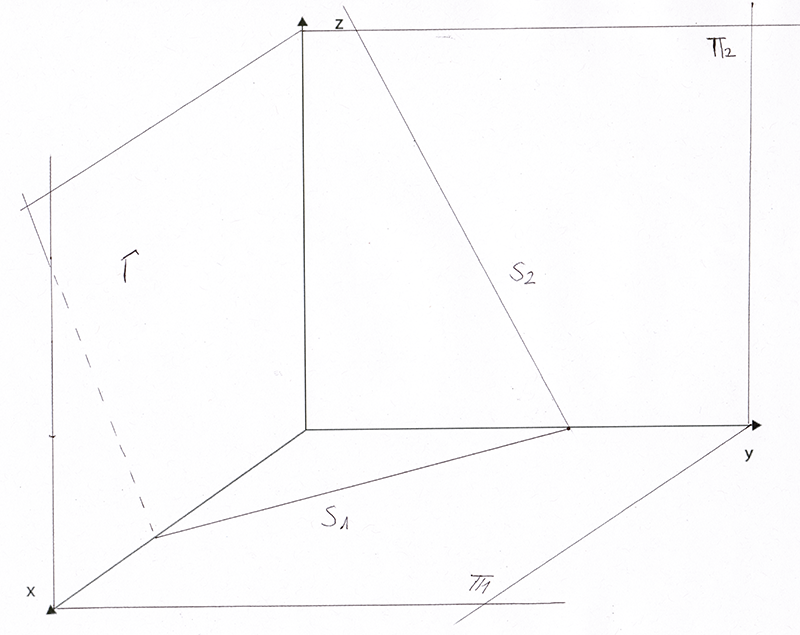
\includegraphics[width=0.8\textwidth]{imgs/Spurgeraden.png}
\end{center}
\begin{eqnarray*}
	s_1 = \Gamma \cap \Pi_1 \text{erster Spurgerade}\\
	s_2 = \Gamma \cap \Pi_2 \text{zweiter Spurgerade}
\end{eqnarray*}
\begin{myexample}
	Berechne die erste Spur von
	\begin{eqnarray*}
		\Gamma: \vec{p} = \begin{pmatrix}2\\5\\-3\end{pmatrix}+\lambda\begin{pmatrix}-1\\1\\1\end{pmatrix}+\mu \begin{pmatrix}2\\4\\3\end{pmatrix}
		\shortintertext{es ist}
		\Pi_1: z=0 
		\shortintertext{also muss}
		-3+\lambda + 3\mu = 0
		\shortintertext{sein. Also}
		\lambda = 3-3\mu
		\shortintertext{und damit}
		x = 2 -(3-3\mu) + 2 \mu = -1 + 5\mu\\
		y = 5+ 3-3\mu + 4\mu = 8+ \mu
		\shortintertext{also ist die erste Spur}
		s_1: \vec{p} = \begin{pmatrix}-1\\8\\0\end{pmatrix}+\mu\begin{pmatrix}5\\1\\0\end{pmatrix}
	\end{eqnarray*}
\end{myexample}
\subsubsection{Lage dreier Ebenen}
\begin{center}
	 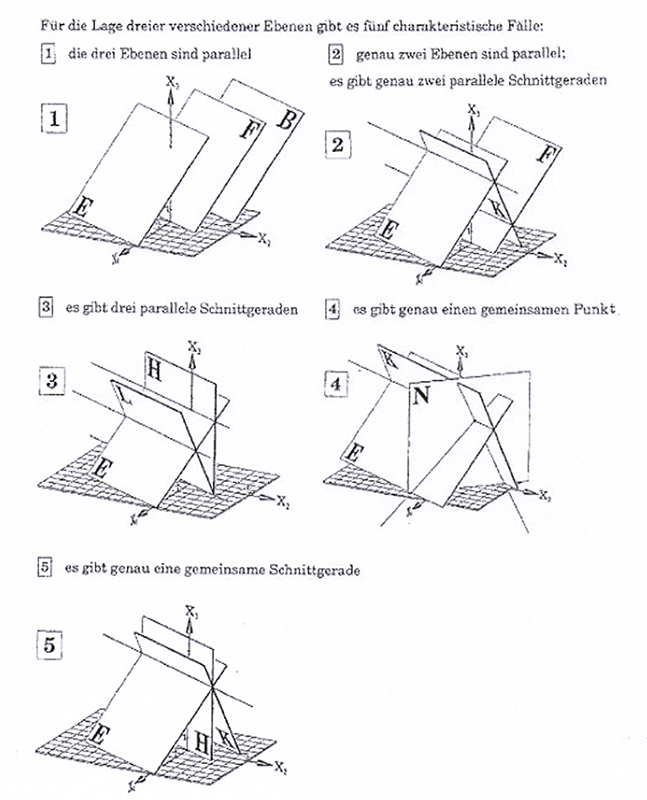
\includegraphics[width=\textwidth]{imgs/lage_drei_ebenen.png}
 \end{center}
 Sind 3 Ebenene parallel, so sind die Koordinatengleichungen
 \begin{eqnarray*}
 	\Sigma:& x-y+2z-4=0\\
 	\Omega: &2x-2y+4z -8 = 0\\
 	\Gamma: &3x-3y+6z-12=0
 \end{eqnarray*}
 \begin{myexample}
 	Berechne den Schnittpunkt der drei Ebenen
 	\begin{eqnarray*}
 		\Lambda:& 2x+y+5z+17+0 = 0\\
 		\Omega: &x+2y+z-2=0\\
 		\Psi: & 2x+5y+z-1=0
 	\end{eqnarray*}
 	Existiert kein solcher Schnittpunkt, so ist die gegenseitige Lage der drei Ebenen und eventuelle Schnittgeraden zu bestimmen.
 	\subsubsection{Parallel}
 	Keine zwei der drei Ebenen sind parallel. Also suchen wir einen Schnittpunkt
 	\subsubsection{Schnittpunkt}
 	\begin{eqnarray*}
 		\begin{tabular}{|l|c}
 			$2x+y+5z+17= 0$&$(1)$\\
 			$x+2y+z-2=0$&$(2)$\\
 			$2x+5y+z-1=0$&$(3)$
 		\end{tabular}\\
 		\\
 		(1)-(3): -4y +4z+18 = 0\\
 		-2y+2z+9= 0\\
 		(1)-2(2): -3y + 3z + 21 = 0
 		\shortintertext{also}
 		\begin{vmatrix}
 			y-z -\frac{9}{2} = 0\\
 			y-z-7 = 0
 		\end{vmatrix}
 	\end{eqnarray*}
 	Was ein Wiederspruch ist.\\
 	Nun müssen wir die Schnittgerade suchen.
 	\subsubsection{Schnittgerade}
 	$\Lambda$ und $\Delta$ mit $x = \alpha$ wird 
 	\begin{eqnarray*}
 		\begin{tabular}{|l|c}
 			$2\alpha+y+5z+17=0$&$(1$)\\
 			$\alpha +2y +z -2 = 0$&$(2)$\\
		\end{tabular}\\
		\\
 		2(1)-(2): \alpha+9z +36 = 0\\
 		9z=-36 -3\alpha\\
 		z = -4-\frac{\alpha}{3}
 		\shortintertext{und}
 		(1)-5(2): -3a -9y + 27 = 0\\
 		9y = 27-3\alpha\\
 		y= 3- \frac{\alpha}{3}
 		\shortintertext{somit ist}
 		s_1: \vec{p} = \begin{pmatrix}0\\3\\-4\end{pmatrix}+\alpha\begin{pmatrix}1\\-\frac{1}{3}\\-\frac{1}{3}\end{pmatrix}
 	\end{eqnarray*}
 	$\Delta$ und $\Psi$ mit $y= \beta$ wird
 	\begin{eqnarray*}
 		\begin{tabular}{l|c}
 			$x+2\beta+z-2 = 0$&(1)\\
 			$2x+5\beta+z -1 = 0$&(2)\\
 		\end{tabular}\\
 		(1)-(2): -x-3\beta-1= 0\\
 		x = -1-3\beta\\
 		2(1)-1: -\beta +z-3 =0\\
 		z=3+\beta
 		\shortintertext{und damit}
 		s_2:\vec{p}= \begin{pmatrix}-1\\0\\-3\end{pmatrix}+\beta\begin{pmatrix}-3\\1\\1\end{pmatrix}
	\end{eqnarray*}
	Also ist $s_1 \parallel s_2$\\
	Falls der rägerpunkt von $s_1$ auf $s_2$ , so sind die Geraden identisch-
	\begin{eqnarray*}
		\begin{pmatrix}0\\3\\-4\end{pmatrix} = \begin{pmatrix}-1\\0\\-3\end{pmatrix}+\beta\begin{pmatrix}-3\\1\\1\end{pmatrix}
		\shortintertext{komponentenweise}
		\begin{tabular}{|l|l}
			$0=-1-3\beta$& $\to \beta = -\frac{1}{3}$\\
			$3= 0+\beta$&$\to \beta = 3$\\
			$-4 = 3 + \beta$&$\to \beta = -7$
		\end{tabular}
	\end{eqnarray*}
	Also ist der Trägerpunkt von 
	\begin{equation*}T_{s_1} \in s_2\end{equation*}
	Damit ist klar, dass die drei Ebenen so liegen, dass die drei Schnittgeraden parallel sind.\\
	Die dritte Schnittgerade finden wir mit
	\begin{eqnarray*}
		\begin{tabular}{|l|c}
			$2x+y+5z+17=0$&$(1)$\\
			$2x+5y+z -1 = 0$&$(2)$
		\end{tabular}\\
		\\
		(1)-(2):\\
		-4y+4z+18=0\\
		2y-2z-9= 0\\
		y = \frac{9}{2}+z
		\shortintertext{und}
		5(1)-(2):\\
		8x+24z+86=0\\
		8x-86-24z\\
		x=-\frac{43}{4}-3z
		\shortintertext{also}
		s_3: \vec{p}= \begin{pmatrix}-\frac{43}{4}\\\frac{9}{2}\\0\end{pmatrix}+z\begin{pmatrix}-3\\1\\1\end{pmatrix}
	\end{eqnarray*}
 \end{myexample}
\newpage
 \section{Normalen und Abstandsprobleme}
\begin{center}
	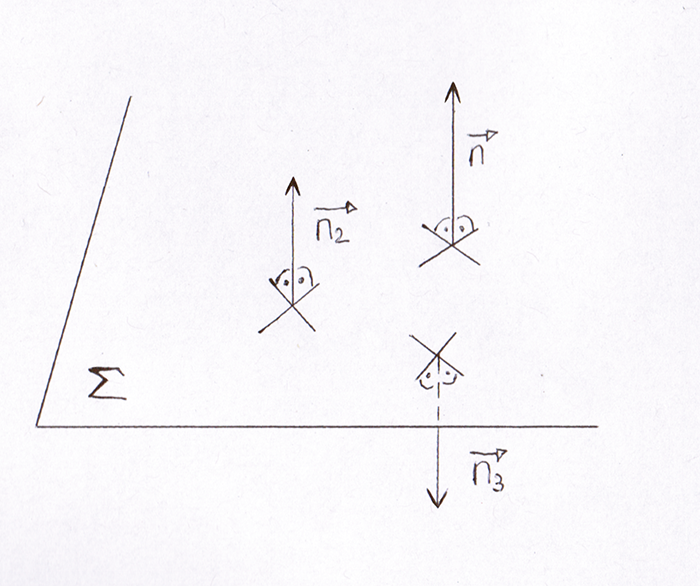
\includegraphics[width=0.8\textwidth]{imgs/Normalenvektor1.png}
\end{center}
 \begin{mydef}
 	Einen Vektor $\vec{n}$, der senkrecht zu einer Ebene $\Sigma$ steht, heisst \underline{Normalenvektor} von $\Sigma$
 \end{mydef}
Kennen wir einen Normalenvektor $\vec{n} = \begin{pmatrix}n_1\\n_2\\n_3\end{pmatrix}$ und einen Punkt $P(p_1/p_2/p_3)$ einer Ebenen $\Sigma$ und suchen einen beliebeigen Punkt $A(x/y/z)$ von $\Sigma$\\
\begin{center}
	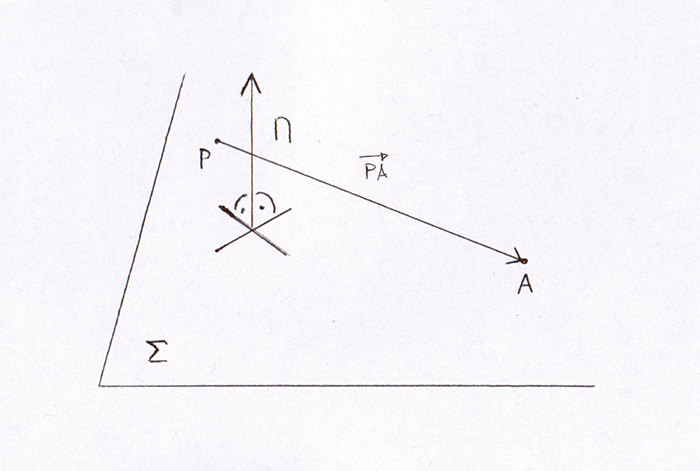
\includegraphics[width=0.8\textwidth]{imgs/Normalenvektor2.png}
\end{center}
So ist
\begin{eqnarray*}
	\vec{PA} \perp \vec{n}
	\shortintertext{also}
	\vec{PA}''\vec{n} &=& 0
	\shortintertext{mit}
	\vec{PA} &=& \begin{pmatrix}x-p_1\\y-p_2\\z-p_3\end{pmatrix}
	\shortintertext{also wir}
	\vec{PA} * \vec{n} &=& (x-p_1)n_1+(y-p_2)n_2+(z-P_3)n_3\\
	&=&n_1x+n_2y+n_3z-(n_1p_1+n_2p_2+n_3p_3)\\
	&=& 0
	\shortintertext{Vergleichen wir mit der Koordinatengleichung}
	\Sigma&:& ax+by+cy+d=0
	\shortintertext{so sehen wir, dass}
	a&=&n_1, b=n_2,c=n_3
	\shortintertext{und}
	d &=& (n_1p_1+n_2p_2+n_3p_3)
	\shortintertext{ist. Aber es ist}
	\vec{n} &=& \begin{pmatrix}n_1\\n_2\\n_3\end{pmatrix}
	\shortintertext{Also besitzt diese Ebene}
	\Sigma&:& ax+by+cz+d = 0
	\shortintertext{den Normalenvektor}
	\vec{n} &=& \begin{pmatrix}a\\b\\c\end{pmatrix}
\end{eqnarray*}
\begin{myexample}
Suchen wir die Parametergleichung der Senkrechten (Normalen, Lot) zur Ebene
$\Sigma: 4x+3y-z+11=0$ wenn $M(5/-2/1)$ auf dem Lot liegen soll.
\begin{center}
		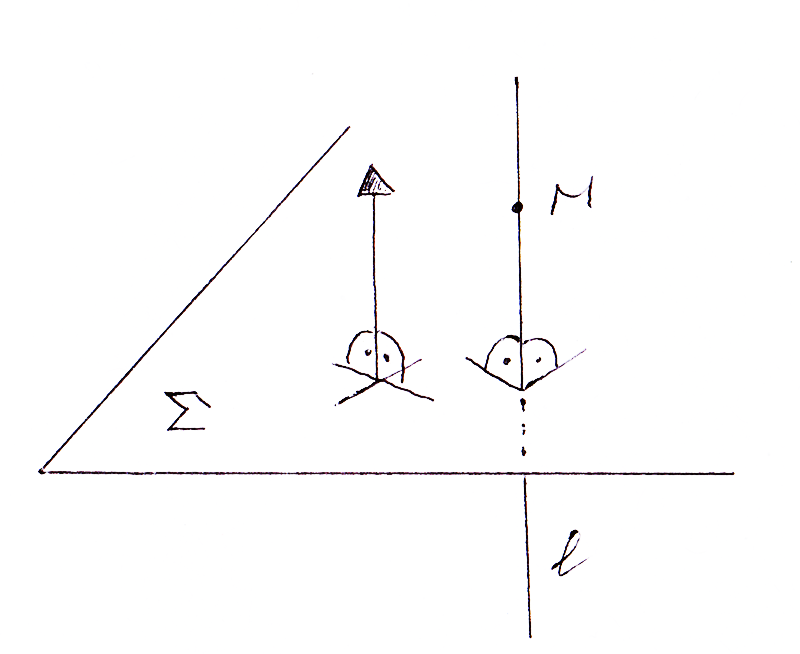
\includegraphics[width=0.8\textwidth]{imgs/Normalenvektor_Beispiel_1.png}
	\end{center}
\begin{equation*}
 	l: \vec{p} = \begin{pmatrix}5\\-2\\1\end{pmatrix}+\lambda\begin{pmatrix}4\\3\\-1\end{pmatrix} = 		\vec{m}+ \lambda\vec{n}
\end{equation*}
\end{myexample}
\begin{myexample}
	Welche Koordinatengleichung besitzt dijenige Ebene $\Gamma$, die $A(4/1/1)$ enthält und senkrecht zu $g: \vec{p} = \begin{pmatrix}-3\\5\\7\end{pmatrix}+\lambda\begin{pmatrix}4\\5\\2\end{pmatrix}$ stehen soll.\\
	\begin{center}
		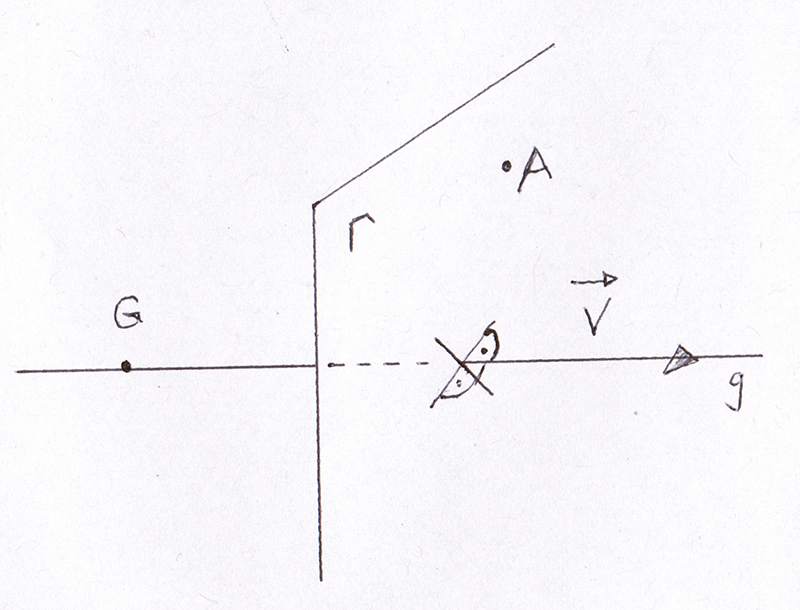
\includegraphics[width=0.8\textwidth]{imgs/Normalenvektor_Beispiel_2.png}
	\end{center}
	$\Gamma$ ist eine \underline{Normalenebene} zu g\\
	$\vec{v}$ ist ein Normalenvektor von $\Gamma$\\ alos
	\begin{eqnarray*}
		\Gamma: 4x+5y+2z+d = 0
		\shortintertext{Da}
		A \in \Gamma
		\shortintertext{setzen wir A in die unfertige Koordinatengleichung ein, wird}
		4*4+5*1+2*1+d = 0\\
		16+5+2+d = 0\\
		23+d = 0\\
		d = 23
		\shortintertext{somit ist die Koordinatengleichung von $\Gamma$}
		\Gamma: 4x+5y+2z-23 = 0
	\end{eqnarray*}
\end{myexample}
\newpage
\subsection{Zwischenwinkel}
$\vec{n}$ kann beliebig platziert werden.\\
\begin{center}
	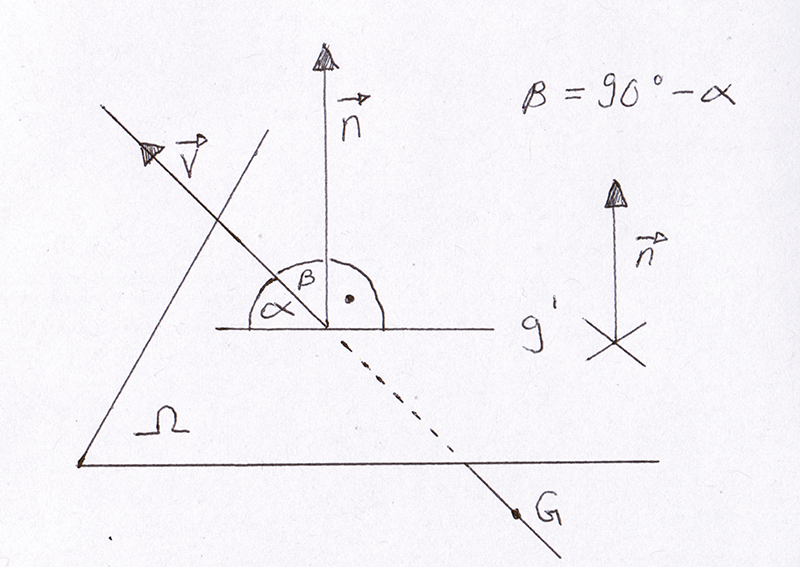
\includegraphics[width=0.8\textwidth]{imgs/Zwischenwinkel1.png}
\end{center}
$g'$ heisst \underline{Normalprojektion} von g auf $\Omega$.
Es ist
\begin{eqnarray*}
	cos(90\circ - \alpha)  = \frac{\vec{n}*\vec{v}}{|\vec{n}|*|\vec{v}|}
	\shortintertext{aber, weil wir die Richtung nicht kennen}
\end{eqnarray*}
	\begin{center}
		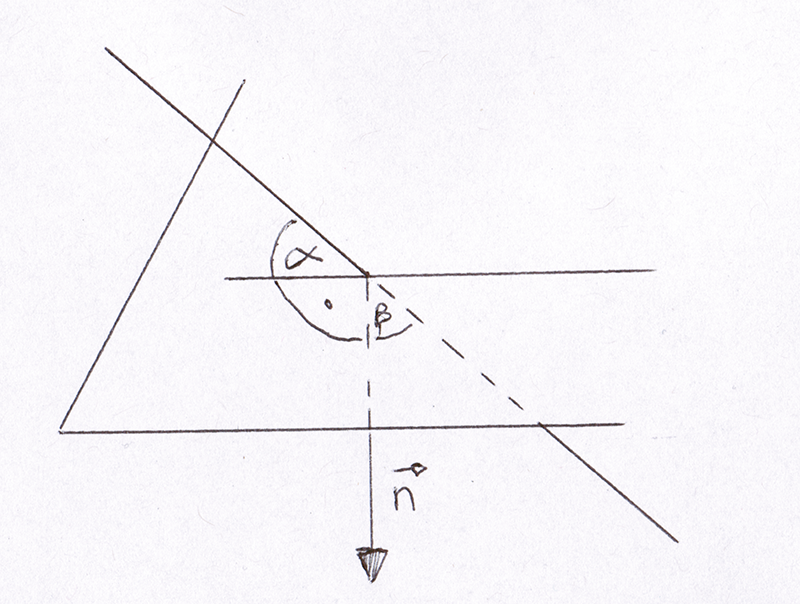
\includegraphics[width=0.8\textwidth]{imgs/Zwischenwinkel2.png}
	\end{center}
also
\begin{equation*}
	cos(90^ \pm \alpha) = \frac{\vec{n}*\vec{v}}{|\vec{n}|*|\vec{v}|}
\end{equation*}
\begin{center}
	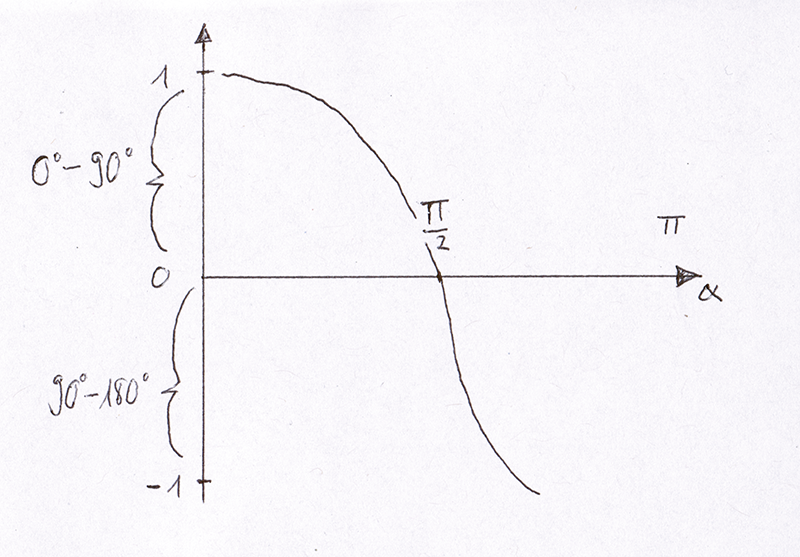
\includegraphics[width=0.8\textwidth]{imgs/CosinusKurve.png}
\end{center}
Es ist
\begin{eqnarray*}
	1 \ge cos(\alpha) \ge 0 \to 0^\circ \le \alpha \le 90^\circ\\
	0 \ge cos(\alpha) \ge -1 \to 90^\circ \le \alpha \le 180^\circ\\
\end{eqnarray*}
\begin{myexample}
	Berechne den Durchstosspunkt und den Zwischenwinkel, wenn\\
	\begin{eqnarray*}
	g: \vec{p}  = \begin{pmatrix}7\\6\\3\end{pmatrix}+\lambda\begin{pmatrix}2\\-1\\-2\end{pmatrix}
	\shortintertext{und}
	\Omega : \vec{p} = \begin{pmatrix}-1\\3\\9\end{pmatrix}+\sigma\begin{pmatrix}1\\-1\\4\end{pmatrix} + \tau\begin{pmatrix}1\\2\\-2\end{pmatrix}
	\end{eqnarray*}
	$\vec{n}$ finden wir entweder mit der Koordinatengleichung oder mit $\vec{n} = \vec{n} \times \vec{v}$\\
	\\
	\textbf{Durchstosspunkt berechnen}\\
	Versuchen wi es mit der Koordinatengleichung. Zuerst müssen wir von der Parametergleichung der Ebene auf die Koordinatengleichung kommen.
	\begin{eqnarray*}
		\begin{tabular}{|l|l}
			$x = -1 + \sigma + \tau$&$(1)$\\
			$y = 3 - \sigma + 2\tau$&$(2)$\\
			$z = 9+ 4\sigma -2\tau$&$(3)$
		\end{tabular}
	\end{eqnarray*}
	\begin{eqnarray*}
		(2)+(3)&:& y+z = 12 + 3 \sigma\\
		2(1)+(3)&:& 2x+z = 7 + 6\sigma\\
		&&2y-2x+z= 17\\
		&&2y-2x+z -17 = 0\\
		\\
		\Omega &:& -2x + 2y +z -17 = 0\\
		\Omega &:& 2x -2y -z +17 = 0
		\shortintertext{mit}
		g&:&x = 7+2y\\
		&&y = 6-\lambda\\
		&&z = 3-2\lambda
	\end{eqnarray*}
	wird dann also
	\begin{eqnarray*}
		2(7+2\lambda)-2(6-\lambda)-(3-2\lambda)+17 = 0\\
		14+4\lambda -12 + 2 \lambda -3 + 2\lambda = 0\\
		16 + 8 \lambda = -16
		\lambda = -2
		\shortintertext{wir setzen lambda in die Prametergeleichung der Geraden g ein. Damit wird}
		D(3/8/7)
	\end{eqnarray*}
	\textbf{Zwischenwinkel berechnen}\\
	Mit
	\begin{eqnarray*}
		\vec{n} = \begin{pmatrix}2\\-2\\-1\end{pmatrix}, \vec{v} = \begin{pmatrix}2\\-1\\-2\end{pmatrix}
		\shortintertext{wird}
		\vec{n}* \vec{v} = 4+2+2 = 8\\
		|\vec{n}| = \sqrt{4+4+1} = \sqrt{9} = 3\\
		|\vec{v}| = \sqrt{4+1+4} = \sqrt{9} = 3
		\shortintertext{und so}
		cos(90^\circ \pm \alpha) = \frac{8}{9}
		\shortintertext{Der Wert liegt zwischen 0 und 1, also liegt der Winkel $\alpha$ zwischen $0^\circ$ und $90^\circ$. Wir müssen also $90^\circ - \alpha$ rechnen}
		cos(90^\circ - \alpha) = \frac{8}{9}\\
		90^\circ - \alpha = 27^\circ.27\\
		\alpha = 62.^\circ.73
	\end{eqnarray*}
\end{myexample}
\newpage
\subsubsection{Zwischenwinkel zweier Ebenen}
\begin{center}
	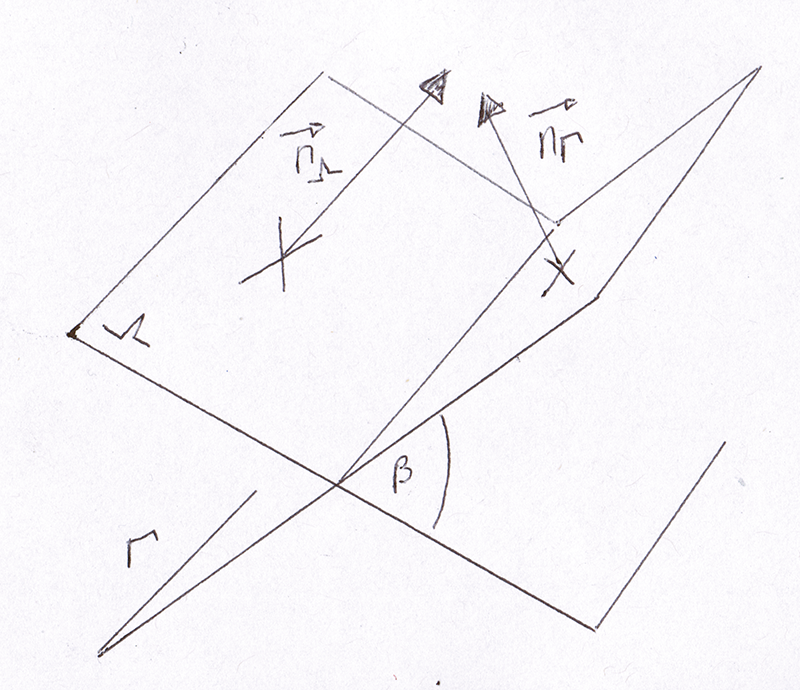
\includegraphics[width=0.8\textwidth]{imgs//Zwischenwinkel_Ebenen.png}
\end{center}
Schnitt
\begin{center}
	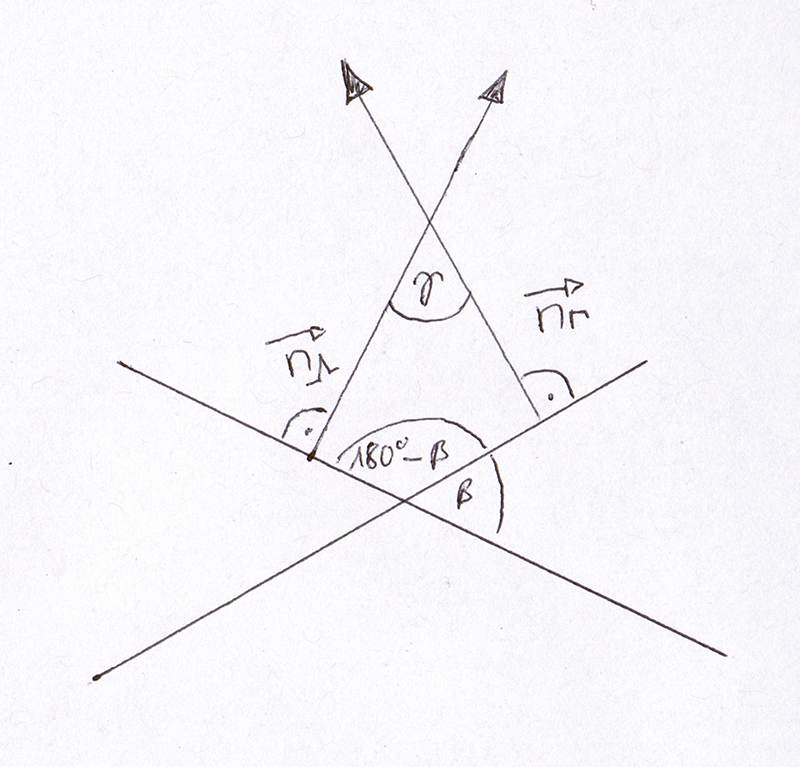
\includegraphics[width=0.8\textwidth]{imgs/Zwischenwinkel_Ebenen_Schnitt.png}
\end{center}
also
\begin{eqnarray*}
	\gamma + 180^\circ + \beta + 90^\circ + 90^\circ = 360^\circ\\
	\gamma - \beta + 360^\circ = 360^\circ\\
	\gamma - \beta = 0
	\gamma = \beta
	\shortintertext{das heisst}
\end{eqnarray*}
\begin{mathbox}
	\begin{equation*}
		cos(\beta) = \frac{\vec{n_\Gamma} * \vec{n_\Lambda}}{|\vec{n_\Gamma}| * |\vec{n_\Lambda}|}
	\end{equation*}
\end{mathbox}
\newpage
\subsection{Spiegelung}
\begin{center}
	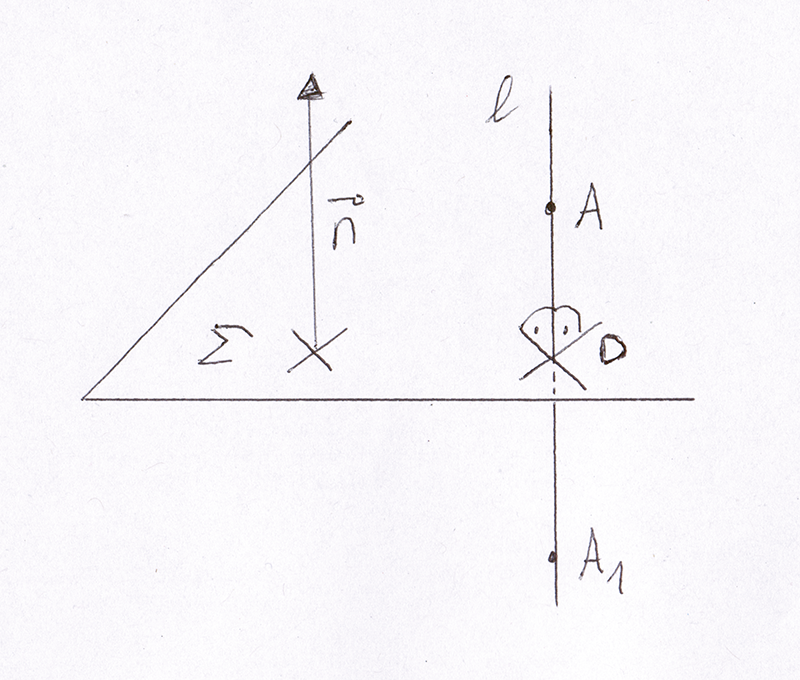
\includegraphics[width=0.8\textwidth]{imgs/Spiegelung_Punkt1.png}
\end{center}
Punkt $A(3/1/-1)$ wird an der Ebene $\Sigma: x+ 2y + 3z -44 = 0$ gespiegelt. Welche Koordinaten hat der Spiegelpunkt $A_1$\\
\\
Es ist also Vekotr $\vec{AD} = \vec{DA_1}$\\
$D$ finden wir mit dem $Lot l$
\begin{eqnarray*}
l: \vec{p} = \begin{pmatrix}3\\1\\-1\end{pmatrix} + \lambda\begin{pmatrix}1\\2\\3\end{pmatrix}\\
\shortintertext{also}
x = 3 + \lambda\\
y = 1 + 2\lambda\\
z = -1 + 3\lambda
\shortintertext{eingesetzt in $\Sigma$}
3 + \lambda + 2(1+2\lambda)+3(-1+3\lambda)-44 = 0\\
3 + \lambda + 2 + 41 -3 + 9 \lambda -44 = 0\\
14\lambda -42 = 0\\
14\lambda = 42
\underline{\lambda = 3}
\end{eqnarray*}
\begin{center}
	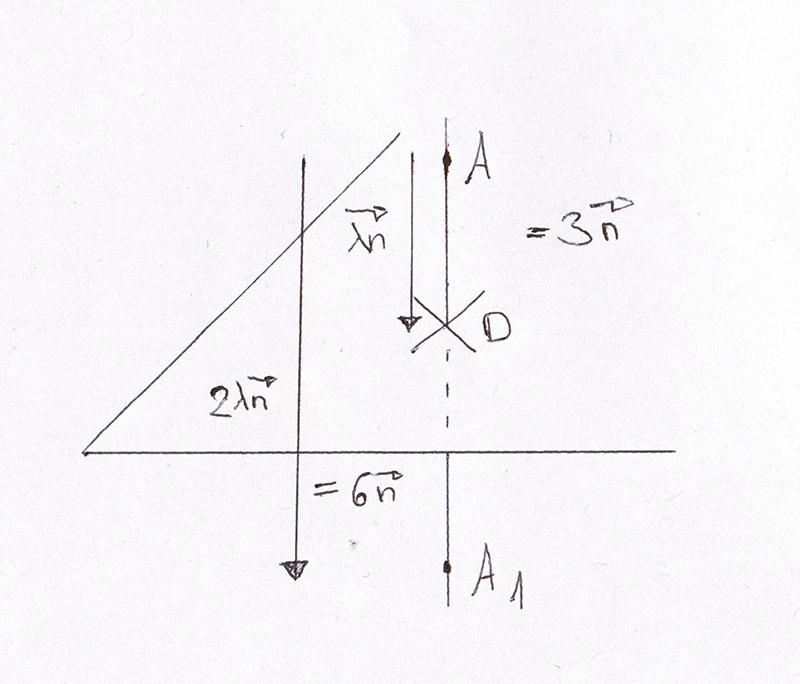
\includegraphics[width=0.8\textwidth]{imgs/Spiegelung_Punkt2.png}
\end{center}
Es ist 
\begin{eqnarray*}
 	\vec{a_1} = \vec{a} + 2 \lambda * \vec{n}
 	\shortintertext{Mit 2 $\lambda$ finden wir}
 	x = 3 + 6 = 9\\
 	y = 1 + 12 = 13\\
 	z = -1 + 18 = 17
 	\shortintertext{also $A_1(9/13/17)$} 
\end{eqnarray*}
\newpage
\subsection{Reflexion}
\begin{center}
	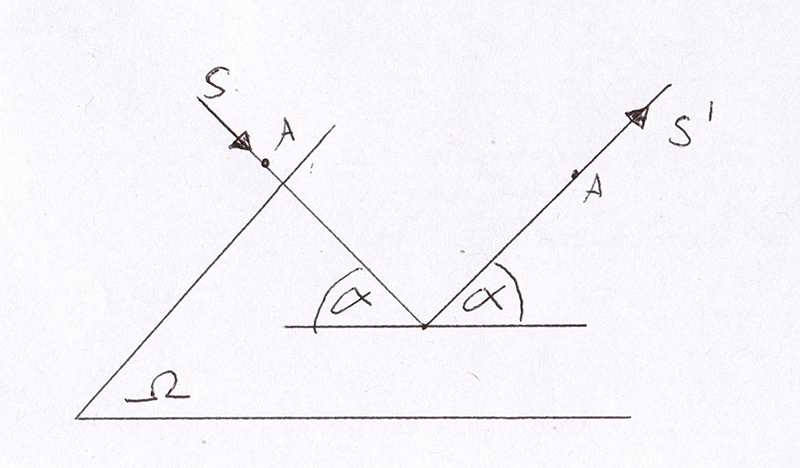
\includegraphics[width=0.8\textwidth]{imgs/Reflexion_Winkel.png}
\end{center}
Einfallswinkel und Ausfallswinkel sind identisch\\
\begin{center}
	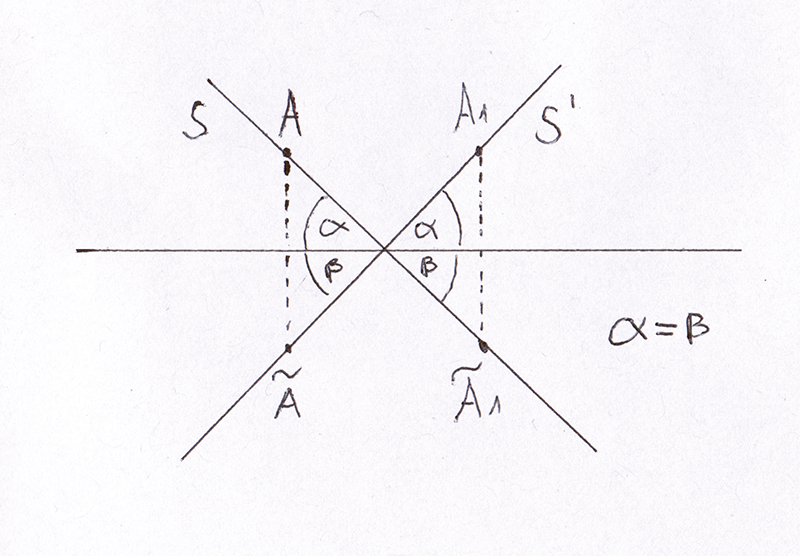
\includegraphics[width=0.8\textwidth]{imgs/Reflexion_Spiegelbild.png}
\end{center}
$s'$ ist das Spiegelbild von $s$\\
\newpage
\begin{myexample}
\begin{center}
	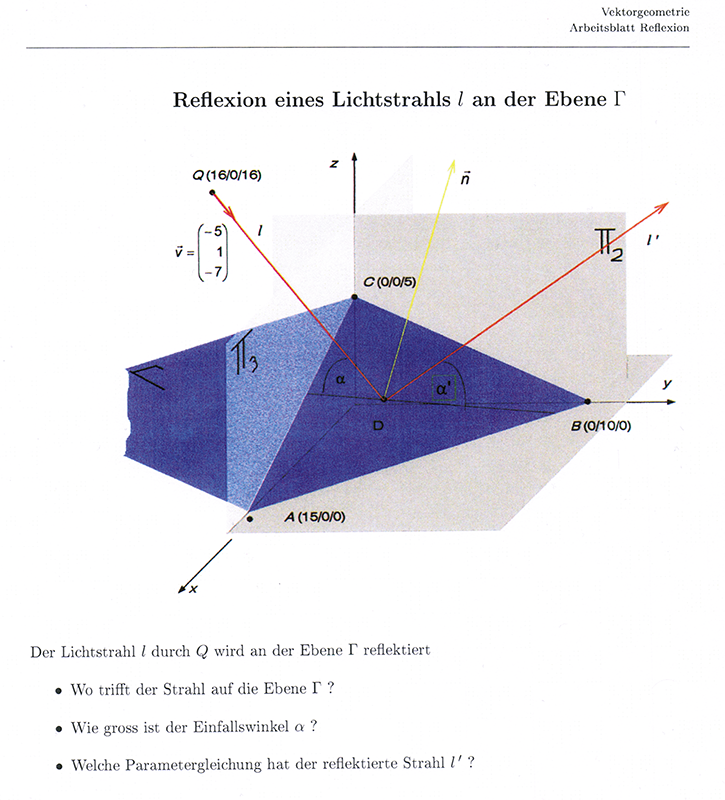
\includegraphics[width=0.8\textwidth]{imgs/Reflexion_Lichtstrahl.png}
\end{center}
\underline{\textbf{Wo trifft der Strahl auf die Ebene $\Gamma$}}\\
Wir suchen die Ebenengleichung
\begin{eqnarray*}
	\Gamma : \vec{p} = \begin{pmatrix}15\\0\\0\end{pmatrix}+ \lambda \begin{pmatrix}-15\\10\\0\end{pmatrix} + \mu \begin{pmatrix}-15\\0\\5\end{pmatrix}\\
	\vec{p} = \begin{pmatrix}15\\0\\0\end{pmatrix}+ \lambda \begin{pmatrix}-3\\2\\0\end{pmatrix} + \mu \begin{pmatrix}-3\\0\\1\end{pmatrix}\\
	\shortintertext{komponentenweise}
	\begin{tabular}{|l|l}
		$x = 15 - 3 \lambda - 3 \mu$ & (1)\\
		$y = 2 \lambda$ & (2)\\
		$z = \mu$ & (3)
	\end{tabular}
	\shortintertext{wir setzen y und z in (1) ein}
	 x = 15 -3 \frac{y}{2} -3z\\
	2x = 30 -3y -6z\\
	\Gamma : 2x + 3y + 6z -30 = 0
	\shortintertext{Mit}
	l : \vec{p} \begin{pmatrix}16\\0\\16\end{pmatrix}+ \lambda  \begin{pmatrix}1-5\\1\\-7\end{pmatrix}
	\shortintertext{wird der Durchstosspunkt D}
	2(16-5\lambda) + 3\lambda + 6(16-7\lambda) -30 = 0 \\
	32 -10\lambda + 3 \lambda + 96 -42\lambda -30 = 0\\
	-49\lambda + 98 = 0\\
	49\lambda = 98\\
	\lambda = 2
	\shortintertext{also}
	D(/6/2/2)
\end{eqnarray*}
Der Strahlt tritt bei D(6/2/2) auf die Ebene $\Gamma$
\clearpage
\noindent
\underline{\textbf{Wie gross ist der Einfallswinkel $\alpha$}}\\
\\
Mit 
\begin{eqnarray*}
	\vec{n} = \begin{pmatrix}2\\3\\6\end{pmatrix}, \vec{v}\begin{pmatrix}-5\\1\\-7\end{pmatrix}
	\shortintertext{wird}
	\vec{n} * \vec{v} = -10 + 3 -42 = -49\\
	|\vec{n}| = \sqrt{4+9+36} = 7\\
	|\vec{v}| = \sqrt{25+1+49} = \sqrt{75}
	\shortintertext{und damit}
	cos(90^\circ + \alpha) = \frac{49}{7 * \sqrt{75}} = \frac{-7}{\sqrt{75}}\\
	90^\circ + \alpha = 143^\circ.93\\
	\alpha = 53^\circ.93
\end{eqnarray*}
\underline{textbf{Welche Parametergleichung hat der Strahl $l'$}}
Wir berechnen nun wie gross $\beta$ ist, damit der Normalenvektor die Ebene $\Gamma$ vom Punkt $Q$ aus schneidet. Wenn wir $\beta$ verdoppeln, werdne wir den gespiegelten Punkt $Q'$ erhalten.\\
\\
Lot $n$ zu $\Gamma$ ist
\begin{eqnarray*}
	n: \vec{p} = \begin{pmatrix}16\\0\\16\end{pmatrix} + \beta\begin{pmatrix}2\\3\\6\end{pmatrix}
	\shortintertext{geschnitten mit $\Gamma$}
	2(16 + 2 \beta) + 3 * 3 \beta + 6(16 + 6\beta) -30 = 0\\
	32 + 4\beta+ 9\beta + 96 + 36\beta -30 = 0\\
	49\beta + 98 = 0\\
	B = -2
	\shortintertext{mit 2$\beta$ im Lot n zu $\Gamma$, wird}
	\begin{vmatrix}
		x = 16 + 2(-4) = 8\\
		y = 3(-4) = -12\\
		z = 16 + 6(-4) = -8
	\end{vmatrix}
	\shortintertext{also $Q'(8/-12/-8)$}
	\shortintertext{Der Richtungsvektor von $l'$ ist}
	 \vec{QD} = \begin{pmatrix}-2\\14\\10\end{pmatrix}
	 \shortintertext{und damit ist}
	 l: \vec{p} = \begin{pmatrix}-8\\-12\\-8\end{pmatrix} + \lambda\begin{pmatrix}-2\\14\\10\end{pmatrix}
	\shortintertext{nach etwas kosmetik erhalten wir}
	 l: \vec{p} = \begin{pmatrix}-8\\-12\\-8\end{pmatrix} + \lambda\begin{pmatrix}-1\\7\\5\end{pmatrix}
	 \shortintertext{Der Aufhängepunkt ist wählbar. Möglich wäre auch}
	  l: \vec{p} = \begin{pmatrix}6\\2\\2\end{pmatrix} + \lambda\begin{pmatrix}-1\\7\\5\end{pmatrix}
	  \shortintertext{was das Ganze etwas anschalicher macht}
\end{eqnarray*}
\end{myexample}
\newpage
\subsection{Abstand}
\begin{center}
	 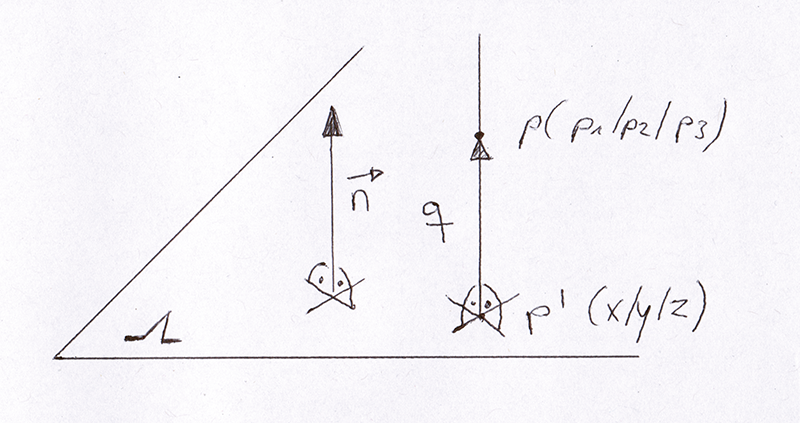
\includegraphics[width=0.8\textwidth]{imgs/Abstand.png}
\end{center}
Ist
\begin{eqnarray*}
	\Lambda: ax + bx + cz + d = 0
	q = |\vec{pp'}|
	\shortintertext{mit Hilfe des Skalarprodukts}
	\vec{pp'} * \vec{n} = |\vec{pp'}| * |\vec{n}| * \cos(\phi)
	\shortintertext{Es ist}
	\phi = 0^\circ \lor \phi = 180^\circ
	\shortintertext{also}
	\vec{pp'} * \vec{n} = |\vec{pp'}| * |\vec{n}| * (\pm 1)
	\shortintertext{mit}
	\vec{n} = \begin{pmatrix}a\\b\\c\end{pmatrix}
	\shortintertext{wird}
	\vec{pp'} * \vec{n} = |\vec{pp'}| * \sqrt{a^2+b^2+c^3}
	\shortintertext{weiter ist}
	\vec{pp'} = \begin{pmatrix}x-p_1\\y-p_2\\z-p_3\end{pmatrix} 
	\shortintertext{also}
	\vec{pp'} * \vec{n} = a(x-p_1) + b(y-p_2) + c(z-p_3)\\
	= ax + by + cz -ap_1 -bp_2-cp_3
	\shortintertext{und}
	p' \in \Lambda
	\shortintertext{also ist}
	ax + by + cz = -d
	\shortintertext{und damit}
	\vec{pp'} * \vec{n} = -d -ap_1-bp_2-cp_3
	\shortintertext{womit wir}
	-d -ap_1 -bp_2 -cp_3 = |\vec{pp'}| * \sqrt{a^2+b^2+c^3}
	\shortintertext{und so wird}
	|\vec{pp'}| = \frac{ap_1+bp_2+cp_3 +d}{\sqrt{a^2+b^2+c^3}}
\end{eqnarray*}
\begin{myexample}
	Welcher Abstand hat Punkt $P(-3/2/2)$ von der Ebene $\Lambda: 6x -6y + 7z + 22 = 0$?
	\begin{eqnarray*}
		q = \frac{|(6*-3)+(-6*2)+(7*2)+22|}{\sqrt{(6)^2+(-6)^2+(7)^2}}\\
		= \frac{|-18-12+14+22|}{\sqrt{36+36+49}}\\
		= \frac{6}{\sqrt{121}}\\
		= \frac{6}{11}
	\end{eqnarray*}
\end{myexample}
Wir finden also den Abstand $q$ eines Punktes von einer Ebene, wenn wir die Koordinaten in die Ebenengleichung einsetzen und dann durch $\vec{n}$ dividieren.
\begin{equation*}
	q = \frac{|ap_1+bp_2+cp_3+ d|}{|\vec{n}|}
\end{equation*}
\begin{mydef}
	Wir nennen 
	\begin{equation*}
		\Sigma: \frac{ax+by+cz+d}{|\vec{n}|} = 0
	\end{equation*}
	Die \underline{Hesse Normalform (HNF} von $\Sigma$ 
\end{mydef}
\begin{myexample}
	Welche Koordinatengleichung hat die Parallelebene in Abstand 5 zur Ebene $\Omega: 6x+ 2y -3z -14 = 0$?\\
	\begin{center}
		 \includegraphics[width=0.8\textwidth]{imgs/Abstand_Ebenen.png}
	\end{center}
	\begin{eqnarray*}
		HNF \Omega: \frac{6x + 2y -3z -14}{\sqrt{36+ 14 + 9}}
		P \in \Sigma
		\shortintertext{ergibt}
		\frac{|6x + 2y -3z -14|}{\sqrt{49}} = 5
		\shortintertext{also}
		\frac{6x + 2y -3z -14}{7} = \pm 5
		\shortintertext{und so}
		\Sigma_1 : 6x + 2y -3z -14 = 35\\
		\Sigma_1 : 6x + 2y -3z -49 = 0\\
		\shortintertext{oder}
		\Sigma_2 : 6x + 2y -3z -14 = -35\\
		\Sigma_2 : 6x + 2y -3z +21 = 0\\
	\end{eqnarray*}
\end{myexample}
\clearpage
\begin{myexample}
	Welchen Abstand hat die Ebene $\Omega: 2x -y + 2z + 15 = 0$ vom Ursprung?
	\begin{equation*}
		q = \frac{15}{\sqrt{(2)^2+(-1)^2+(2)^2}} = \frac{15}{3} = 5
	\end{equation*}
	Wir sehen die Variable d der Ebenengleichung, definiert den Abstand zum Ursprungspunkt.\\
	d ist ein Vielfaches von $|\vec{n}|$
\end{myexample}
\clearpage
Die HNF lässt sich auch im $R^2$ verwenden.\\
Ist
\begin{eqnarray*}
	y = mx + q
	\shortintertext{die \underline{explizite},und}
	ax + by + c = 0
	\shortintertext{die \underline{implizite} Geradengleichung, so ist die HNF}
	\frac{ax + by + c}{\sqrt{a^2+b^2}}
\end{eqnarray*}
\begin{myexample}
	Welchen Abstand hat die Gerade $g: 4x -3y + 30 = 0$ vom Ursprung?
	\begin{eqnarray*}
		\frac{4x -3y + 30}{\sqrt{(4)^2+(-3)^2}} = 0
		\shortintertext{Setzen wir nun den Urpsurngspunkt $\begin{pmatrix}0\\0\end{pmatrix}$ ein}
		q = \frac{30}{\sqrt{25}} = \frac{30}{25} = 6
	\end{eqnarray*}
\end{myexample}
\begin{myexample}
	Wie lang ist $ha$ im Dreieck $ABC$, wenn $A(-4/-1)$, $B(5/2)$ und $C(-1/10)$ ?\\
	\begin{center}
		 \includegraphics[width=0.8\textwidth]{imgs/Abstand_Ebenen_Beispiel_2.png}
	\end{center}
	$ha$ ist der Abstand von a zu A.\\
	Ist
	\begin{eqnarray*}
		a: y = mx + q
		\shortintertext{so finden wir mit B und C}
		\begin{tabular}{|l|l}
			$2 = 5m + q$ 		& 	$(1)$\\
			$10 = -m + q$	&	$(2)$
		\end{tabular}
		\shortintertext{(1)-2}
		-8 = 6m\\
		m = -\frac{4}{3}
		\to
		10 = \frac{4}{3} + q\\
		\frac{26}{3} = q
		\shortintertext{Also}
		a: y = -\frac{4}{3}x + \frac{26}{3}
		\shortintertext{implizit}
		3y = -4x + 26\\
		4x + 3y -26 = 0
		\shortintertext{A in die HNF von a einsetzen}
		ha = \frac{|4(-4)+3(-1)-26)|}{\sqrt{4^2+3^2}}\\
		= \frac{|-45|}{\sqrt{25}} \\
		= 9
	\end{eqnarray*}
\end{myexample}
\newpage
\chapter{Kreise und Tangenten}
\begin{center}
	 \includegraphics[width=0.8\textwidth]{imgs/Kreis_Koordinatengleichung.png}
 \end{center}
\underline{Koordinatengleichung} des Kreises mit Zentrum im Ursprung\\
\\
\begin{mathbox}
	\begin{equation*}x^2 + y^2 = r^2\end{equation*}
\end{mathbox}
\noindent
Wählen wir en Winkel $\lambda$ als Paramater, so erhalten wir\\
\begin{center}
	 \includegraphics[width=0.8\textwidth]{imgs/Kreis_Parametergleichung.png}
\end{center}
\begin{mathbox}
	\begin{eqnarray*}
 		x = r * \cos(\lambda)\\
 		y = r * \sin(\lambda)
 		0^\circ < \lambda < 360^\circ\\
 		\vec{p} = \begin{pmatrix}x\\y\end{pmatrix} = r \begin{pmatrix}\cos(\lambda)\\\sin(\lambda)\end{pmatrix}\\
 		\shortintertext{die \underline{Parametergleichung des Kreises}}
 	\end{eqnarray*}	
 \end{mathbox}
 \noindent
 Ist $M(x_m/y_m)$ der Mittelpunkt des Kreises\\
\begin{center}
	 \includegraphics[width=0.8\textwidth]{imgs/Kreis_Parametergleichung_Beliebig.png}
\end{center}
 So ist
 \begin{eqnarray*}
 	\vec{p} = \vec{m} + \vec{r}
 	\shortintertext{also}
\end{eqnarray*}
\begin{mathbox}
 	\begin{eqnarray*}
 		\begin{pmatrix}x\\y\end{pmatrix} = \begin{pmatrix}x_m\\y_m\end{pmatrix} + \begin{pmatrix}r \cos(\lambda)\\r \sin(\lambda)\end{pmatrix}
 		x = x_m + r \cos(\lambda)\\
 		y = y_m + r \sin(\lambda)\\
 		0^\circ < r < 360^\circ\\
 		\shortintertext{die \underline{Parametergleichung eines beliebigen Kreises}}
 	\end{eqnarray*}
\end{mathbox}
so wird 
\begin{eqnarray*}
 	x - x_m = r \cos(\lambda)\\
 	y - y_m  = r \sin(\lambda)
 	\shortintertext{also}
 	(x - x_m)^2 = r^2 \cos^2(\lambda)\\
 	(y - y_m)^2 = r^2 \sin^2(\lambda)
 	\shortintertext{und so}
 	(x - x_m)^2 + (y -y_m)^2 = r^2(\cos^2(\lambda) + \sin^2(\lambda))
 	\shortintertext{durch die Trigonometrie finden wir}
\end{eqnarray*}
\begin{mathbox}
 	\begin{eqnarray*}
 		(x - x_m)^2 + (y -y_m)^2 = r^2(1)\\
 		(x - x_m)^2 + (y -y_m)^2 = r^2\\
 		\shortintertext{die Koordinatengleichung eines Kreises mit Mittelpunkt $M(x_m/y_m)$}
 	\end{eqnarray*}
\end{mathbox}
\begin{myexample}
 	Welche Koordnatengleichung hat der Kreis $K$ mit $M(2/-3)$ und Radius $r = 7$?
 	\begin{eqnarray*}
 		(x-2)^2 + (y+3)^2 = 49
 		\shortintertext{was ausgerechnet}
 		x^2 -4x + 4 + y^2 + 6y + 9 = 49\\
 		x^2 + y^2 -4x + 6y -36 = 0
 		\shortintertext{ergibt.}
 	\end{eqnarray*}
\end{myexample}
\begin{myexample}
     	Bestimme Mittelpunkt und Radius, wenn
   	\begin{enumerate}
 		\item
 			\begin{eqnarray*}
 				x^2 + y^2 -12x + 10y + 52 = 0\\
 				\shortintertext{wir ergänzen quadratisch}
 				x^2 -12x + 36 + y^2 + 12y + 25 = -52 + 36 + 25\\
 				(x-6)^2 + (y+5)^2 = 9
 				\shortintertext{also}
 				M(6/-5), r = 3
 			\end{eqnarray*}
		\item
 			\begin{eqnarray*}
 				x^2 + 2y^2 + 4x -5y + 7 = 0\\
 				x^2 + 4x+ 4 + 2y^2 -5y + ? = -7\\
 				\shortintertext{Keine Kreisgleichung, sondern eine Ellipse}
 			\end{eqnarray*}
		\item
			Wenn der Kreis die X-Achse berührt und die Punkte $A(1/4)$, $B(-1/2)$ auf der Peripherie liegen soll.\\
			\begin{center}
				 \includegraphics[width=0.8\textwidth]{imgs/Kreis_Beispiel_2c.png}
			\end{center}
			\begin{eqnarray*}
				K: (x - x_m)^2 + (y -y_m)^2 = r^2\\
				A \in K : (1 -x_m)^2 + (4 -y_m)^2 = r^2\\
				B \in K : (-1 -x_m)^2 + (2 -y_m)^2 = r^2\\
				\shortintertext{und}
				y_m = r
				\shortintertext{also}
				\begin{tabular}{|l|l}
					$1 - 2x_m + x^2m + 16-8r + r^2 = r^2$ &$ (1)$\\
					$1 + 2x_m + x^2_m + 4 -4r + r^2 = r^2 $&$ (2) $
				\end{tabular}\\
				\\
				\begin{tabular}{|l|l}
					$x^2m - 2x_m -8r + 17 = 0 $& $(1)$\\
					$x^2_m + 2x_m -4r + 5 = 0$ &$ (2)$ 
				\end{tabular}\\
				\\
				(1)-2(2):\\
				-x^2_m -6x_m + 7 = 0\\
				x^2_m + 6x_m -7 = 0\\
				(xm_1 + 7)(x_m -1) = 0\\
				x_{m1} = -7\\
				x_{m2} = 1
				\shortintertext{in (2) mit $x_{m1}$ erhalten wir} 
				49 -14 -4r_1 + 5 = 0\\
				40 = 4r_1
				r_1 = 10
				\shortintertext{und in (2) mit $x_{m2}$ erhalten wir}
				1 + 2 -4r_2 + 5 = 0\\
				8 = 4r_2\\
				r_2 = 2
				\shortintertext{führt uns also zu}
				ym_1 = 10,  ym_2 = 2
				\shortintertext{also}
				M_1(-7/10), r_1 = 10\\
				M_2(1/2), r_2 = 2
			\end{eqnarray*}
	\end{enumerate}
 \end{myexample}
 \clearpage
 \begin{myexample}
 Welches Zentrum hat derjenige Kreis durch $P(3/7)$, der den Kreis $(x-4)^2 + (y-1)^2 = 9$ von aussen und ausserdem die x-achse berührt?\\
 BILD TO SCAN\\
 	\begin{eqnarray*}
 		\shortintertext{Wir definieren die Ausgangslage:}
 		y_m = r\\
 		\shortintertext{und}
 		|\vec{MZ}| = r * \rho
 		\shortintertext{wobei $\rho$ der Radius des gegebenen kleinen Kreises ist, also}
 		\rho = 3
 		\shortintertext{Wir können den Radius aus der Kreisgleichung entnehmen. Mit}
 		Z(4/1), \vec{MZ} = \begin{pmatrix}4 - xm\\ 1 - ym\end{pmatrix}
 		\shortintertext{Punkt $Z$ können wir aus der Kreigleichung entnehmen und so}
 		|\vec{MZ}| = \sqrt{(4 - x_m)^2 + (1-y_m)^2}
 		\shortintertext{also}
 		(4 - x_m)^2 + (1 - r)^2 = (r + 3)^2\\
 		\\
 		\shortintertext{Wir ersetzen $|\vec{MZ}|$ mit (r+3) und erhalten}
 		(r+3)^2 = (4 - x_m)^2 + (1 - r)^2\\
 		r^2 + 6 + 9 = 16 - 8x_m + x_m^2 + 1 + r^2 -2r\\
 		x_m^2 -8x_m -8r + 8 = 0\\
 		\shortintertext{und}
 		P \in K
 		\shortintertext{also}
 		(x_m -3)^2 + (y_m -7)^2 = r^2\\
 		\shortintertext{wir ersetzen $y_m$ mit $r$}
 		(x_m -3)^2 + (r -7)^2 = r^2\\
 		x_m^2 -6x_m + 9 + r^2 -14r + 49 = r^2\\
 		x_m^2 -6x_m -14r + 58 = 0
 		\shortintertext{somit erhalten wir zwei Kreisgleichungen}
 		\begin{tabular}{|l|l}
 			$x_m^2 -8x_m -8r + 8 = 0$ & $(1)$\\
 			$x_m^2 -6x_m -14r + 58 = 0$ &$(2)$
 		\end{tabular}\\
 		-7(1) + 4(2):\\
 		-3x_m^2 + 32x_m + 176 = 0\\
 		3x_m^2 + 32xm + 176 = 0\\
 		\shortintertext{wir ergänzen quadratisch}
 		x_m^2 -\frac{32}{3}x_m + (\frac{32}{6})^2 = \frac{176}{3} + (\frac{32}{6})^2\\
 		(x_m -\frac{32}{6})^2 = \frac{176}{3} + \frac{16^2}{3^2}\\
 		(x_m -\frac{32}{6})^2 = \frac{176*3+256}{9}\\
 		(x_m -\frac{32}{6})^2 = \frac{528+256}{9}\\
 		x_m -\frac{32}{6} = \pm\sqrt{\frac{784}{9}} \\
 		x_m -\frac{32}{6} = \pm \frac{28}{3}\\
 		x_m = \pm \frac{28}{3} +\frac{32}{6}\\
 		\shortintertext{damit erhalten wir}
 		x_{m1} = \frac{28}{3} + \frac{32}{6} = \frac{88}{6} = \frac{44}{3}\\
 		x_{m2} = - \frac{28}{3} + \frac{32}{6} = - \frac{24}{6} = -4\\
 		\\
 		\shortintertext{Wir suchen $y_{m1}$, wir setzen $x_m1$ in die Kreisgleichung}
 		(4 - x_m)^2 + (1 - r)^2 = (r + 3)^2\\
 		\shortintertext{ein. Wir erhalten}
 		(4 -\frac{44}{3})^2 + (1-r)^2 = (r+3)^2\\
 		(\frac{32}{3})^2 + 8 -8r = 0\\
 		\frac{32^2+8*9}{9} -8r = 0\\
 		\frac{32^2+72}{9} -8r = 0\\
 		\frac{1096}{9} -8r = 0\\
 		\frac{1096}{9} = 8r\\ 
 		\frac{1096}{9*8} = r\\
 		\frac{1096}{72} = r\\  
 		\frac{137}{9} = r = y_{m1}
 		\shortintertext{Nun suchen wir $y_{m2}$, wir setzen $x_{m2}$ in die Gleichung} 
 		(4 - x_m)^2 + (1 - r)^2 = (r + 3)^2\\
 		\shortintertext{ein. Wir erhalten}
 		(4-(-4))^2 + 8 -8r = 0\\
 		64 + 8 -8r = 0\\
 		72 = 8r\\
 		9 = r = y_{m2}
 		\shortintertext{also}
 		M_1(\frac{44}{3}/\frac{157}{9}), r_1 = \frac{137}{9}\\
 		M_2(-4/9), r_2 = 9\\
 	\end{eqnarray*}
 \end{myexample}
 \newpage
 \section{Tangenten}
\begin{center}
	 \includegraphics[width=0.8\textwidth]{imgs/tangenten_aufUrsprung.png}
\end{center}
 Mittels Kehrwert finden wir 
\begin{eqnarray*}
	m_t * m_l = -1
	\shortintertext{und}
	m_l = \frac{y_B}{x_B}
	\shortintertext{wird also}
	m_t = -\frac{x_B}{y_B}
	\shortintertext{Ist}
	t: y = m_tx+ q
	\shortintertext{so finden wir mit $B \in t$}
	y_B = m_tx_B + q\\
	y_B - m_tx_B = q
	\shortintertext{also}
	t: y = m_tx + y_B -m_tx_B\\
	y = m_t(x-x_B) + y_B
	\shortintertext{mit}
	m_t = - \frac{x_B}{y_B} (x-x_B) + y_B\\
	yy_B = -xx_B + x^2_B + y^2_B\\
	xx_B + yy_B = x_B^2 + y_B^2
	\shortintertext{und es ist}
	x_B^2 + y_B^2 = r^2
\end{eqnarray*}
also
\begin{mathbox}
	\begin{equation*}t: xx_B + yy_B = r^2\end{equation*}
\end{mathbox}
\begin{myexample}
	Welche Gleichung hat die Tangente im Punkt $B(12/y_B)$ des Kreises $x^2 +y^2 = 169$, wenn $y_B < 0$ sein soll?\\
	\\
	\begin{eqnarray*}
		(12)^2 + y_B^2 = 169\\
		169 -144 = 25 = y_B^2\\
		y_B = \pm 5
		\shortintertext{also}
		B(12/-5)
		\shortintertext{und damit}
		t: 12x -5y = 169\\
		t: 12x -5y -169 = 0
	\end{eqnarray*}
\end{myexample}
\begin{center}
	 \includegraphics[width=0.8\textwidth]{imgs/tangenten_NichtAufUrsprung.png}
\end{center}
Ist 
\begin{equation*}t: (x-x_m)^2 + (y-y_m)^2 = r^2\end{equation*}
so finden wir die Gleichung der Tangente in $B \in K$ analog
\begin{mathbox}
	\begin{equation*}t: (x_B -x_m)(x-x_m)+(y_B -y_m)(y-y_m) = r^2\end{equation*}
\end{mathbox}
\newpage
\begin{center}
	 \includegraphics[width=0.8\textwidth]{imgs/tangenten.png}
\end{center}
Wir versuchen nun die Tangentengleichungen von $t_1$ und $t_2$ herauszufinden.\\
Wir überlegen, dass $r$ der \underline{Abstand} des Mittelpunktes M von den Tangenten $t_1$ und $t_2$ ist.\\
\\
Ist 
\begin{eqnarray*}
	P(-1/-2) \\
	\shortintertext{und}
	K: x^2 + y^2 -20x -16y + 139 = 0\\
	\shortintertext{mit der Tangentengleichung}
	t : y = mx + q
	\shortintertext{und}
	p \in t
	\shortintertext{finden wir}
	-2 = -m+ q\\
	q = m - 2
	\shortintertext{in der expliziten Form also}
	t = mx + m -2
	\shortintertext{in der impliziten Form}
	0 = mx -y + m -2
	\shortintertext{dann ist}
	\vec{n} = \begin{pmatrix}m\\-1\end{pmatrix}
	\shortintertext{damit wird die HNF}
	\frac{mx-y+ m-2}{\sqrt{m^2+1}} = 0
	\shortintertext{Den Mittelpunkt finde wir mit}
	K: x^2 -20x+ y^2 -16y + 139 = 0\\
	\shortintertext{Wir ergänzen quadratisch und erhalten}
	K: x^2 -20x+ 100 + y^2 -16y + 64 + 139 = 0\\
	(x-10)^2 + (y-8)^2 = 25\\
	\to M(10/8), r = 5
	\shortintertext{was eingesetzt in die HNF}
	\begin{vmatrix}\frac{10m -8 + m -2}{\sqrt{m^2 + 1}}\end{vmatrix} = 5
	\shortintertext{ergibt}
	\frac{11m-10}{\sqrt{m^2 + 1}} = \pm 5\\
	11m -10 = \pm 5 \sqrt{m^2 + 1}\\
	(11m -10)^2 = 25 \sqrt{m^2 + 1}\\
	121m^2 -220m + 100 = 25m^2 + 25\\
	96m^2 -220m + 75 = 0\\
	(12m-5)(8m -15) = 0\\
	\to m_1 = \frac{5}{12}, m_2 = \frac{15}{8}
	\shortintertext{Wir haben nun die beiden Steigungen $m_1$ und $m_2$ ausgerechnet. Mit diesen Werten lässt sich nun die Tangentengleichung bestimmen. Wir setzen die Werte in die implizite Tangengleichung ein. Mit $m_1$ wird}
	t_1 : y = \frac{5}{12}x + \frac{5}{12} -2\\
	12y = 5x + 5 -24\\
	\underline{t_1 : 5x -12y -19 = 0}\\
	\shortintertext{mit $m_2$ wird}
	t_2 : y = \frac{15}{8}x + \frac{15}{8} -2\\
	8y = 15x + 15 -16\\
	\underline{t2 : 15x -8y -1 = 0}
\end{eqnarray*}
